\documentclass[a4paper,11pt]{book}
\usepackage{graphicx}
\usepackage{epsf}
\usepackage{tocbibind}
\usepackage{amsmath}
\usepackage{color}
\usepackage{titlesec}
\usepackage{titletoc}
\usepackage{algorithm}
\usepackage{algpseudocode}
\usepackage{tools/fancyhdr}
\usepackage{tools/appendix}
\usepackage{setspace}
\usepackage{subfigure}
\usepackage{enumerate}
\addtolength{\textheight}{1cm}
\addtolength{\textwidth}{0.8cm}
\addtolength{\voffset}{0.2cm}
\setlength{\oddsidemargin}{0.9cm}
\setlength{\evensidemargin}{0.5cm}
%Henry's non-sense:
%\setlength{\oddsidemargin}{1.0cm}
%\setlength{\evensidemargin}{-0.47cm}
%\setlength{\parindent}{0cm}
\newcommand{\clearemptydoublepage}{\newpage{\pagestyle{empty}\cleardoublepage}}


\def\x{{\bf x}}
\def\r{{\bf r}}
\def\rp{{\bf r^\prime}}
\def\rpp{{\bf r^{\prime\prime}}}
\def\rppp{{\bf r^{\prime\prime\prime}}}
\def\u{{\bf u}}
\def\p{{\bf p}}
\def\k{{\bf k}}
\def\q{{\bf q}}
\def\G{{\bf G}}
\def\R{{\bf R}}
\def\Rs{{\mathcal{R}}}
\def\Gp{{\bf G^\prime}}
\def\sig{$\Sigma$}
\def\inveps{\varepsilon^{-1}}
\def\eps{\varepsilon}
\def\symm{\left\{\mathcal{S}|\mathbf{v}\right\}}
\def\S{\mathcal{S}}
\def\rt{\tilde{r}}
\def\pt{\tilde{p}}
\def\T{\hat{T}}
\def\bra{\langle}
\def\ket{\rangle}
\def\field{\hat{\psi}}
\def\cfield{\hat{\psi}^{\dagger}}
\def\I{\hat{I}}
\def\w{\omega}
\def\wp{\omega^\prime}
\def\wc{{\omega_{\rm C}}}
\def\e{{\rm e}}
\def\E{\varepsilon}
\def\Y{\mathcal{Y}}
\def\H{\hat{H}}
\def\v{\mathbf{v}}
\def\Gs{\mathcal{G}}
\def\P{\hat{P}_{\rm occ}}
\def\mos{$\textrm{MoS}_{2}$~}
\def\ws{$\textrm{WS}_{2}$}
\def\ck{c_{\k\uparrow}}
\def\ckp{c^{+}_{\k\uparrow}}
\def\cmk{c_{-\k\downarrow}}
\def\cmkp{c^{+}_{-\k\downarrow}}
\definecolor{yellow}{rgb}{1,1,0}
\definecolor{lightblue}{rgb}{0.6,0.6,0.9}
%\sethlcolor{yellow}


\renewcommand{\thechapter}{\arabic{chapter}}
\renewcommand*{\thesection}{\arabic{section}}
\renewcommand{\thesubsection}{\arabic{section}.\arabic{subsection}}
%\setlength{\cftsecnumwidth}{3em}
\titleformat  {\chapter}[hang]{\bfseries\huge\centering}{\thechapter}{2pc}{}{}
\titlespacing {\chapter}{0pt}{0pt}{16pt}{}
\titleformat  {\section}[hang]{\bfseries\large}{\thesection}{2pc}{}{}
\titlespacing {\section}{0pt}{8pt}{6pt}{}
\titleformat  {\subsection}[hang]{\bfseries}{\thesubsection}{2pc}{}{}
\titlespacing {\subsection}{0pt}{10pt}{10pt}{}

\usepackage[sort&compress]{natbib}
\setlength{\bibsep}{0.0pt}
\bibpunct{[}{]}{,}{n}{,}{,}

\begin{document}
\frontmatter
\title{Electronic Structure From the Perspective of the Local Environment}
\author{Henry Lambert \\
\vspace{0.2cm} \\
King's College London
}

\maketitle
\pagenumbering{roman}
\makeatletter
\tableofcontents

\mainmatter
\pagenumbering{arabic}

\chapter{Introduction}
\section{Electronic Structure for Materials Science}
In 1987 Henry Ehrenreich published an article in Science called
"Electronic Theory for Materials Science". The article begins
with what might now be considered a bold statement:

\begin{quote}
Theoretical Materials Science remains to be invented as a discipline, and for good reason.
\end{quote}

The reason he supplies is that materials processing, historically, was a craft. 
Roman engineers could manufacture concrete which was in some ways superior to that
made today without any specific knowledge of the microstructure of the material.
A blacksmith learned that the hardness of swords and shields could be manipulated 
by the alloying of metals and precise control of heat. This expertise was not accumulated 
based on reasoning from first principles but based on experience, trial and error, 
and general trade craft.

A satisfactory atomic theory and the techniques to solve the equations which arise in that theory
have only arisen in the last 100 years. Over the past 40 years the possibility of constructing
accurate models of materials systems beginning from the arrangment of the constituent atoms has
driven a great deal of what is sometimes called first principles or {\it ab initio} modelling.

The extent to which theoretical materials science as a discipline has evolved is worth examining. 
It is important because the character of this evolution dictates which directions of research may prove most
immediately fruitful. It is also important because it allows researchers to identify the many avenues
where people are going backwards, obscuring knowledge, and in some sense unlearning or convoluting 
what is already understood. 

To chart this evolution we may begin from Ehrenreich's survey of the field from 30 years ago.

Ehrenreich identified four points that characterized the state of the field of material science at the time:
%
\begin{enumerate}[i)]
\item Theory must be closely linked to experiment.
\item Ab initio calculations without approximations are virtually impossible except in model systems.
\item Approximations are frequently based on prior experience rather than on theoretical justification.
\item The study of trends in the properties of homologous materials 
      is a crucial ingredient of a credible theoretical framework.
\end{enumerate}
%

It is worth while considering how the intervening 30 years may have adjusted some of 
these priorities and characterize the current state of the field.

\section{The Rise of the Computer}
The intervening thirty years has seen an enormous extension of 
computing capacity. 

Around the time Ehrenreich was writing an example of a 
state of the art computer would be the Connection Machine.
\footnote{One of the employees at Thinking Machines Corporation,
the company building the connection machine, was Richard Feynman.
For an interesting discussion of the work they
did at Thinking Machines and Feynman's time there see W. Daniel
Hillis' article in Physics Today 42, 2, 78 (1989).
There was a strong focus on design at the company. Some of that
work can be found at Tamiko Thiel's page}%; \url{http://www.tamikothiel.com/theory/cm_txts/di-frames.html}}

The CM-2 was launched in 1987 It was configured with up to 512 MB of RAM and 25 GB of RAID
hard disk space. It had 65K microprocessors (each with 600 bytes of memory). Support for
32 bit floating point operations meant just over 2048 processors in practice per machine.

By contrast a standard HPC machine accessible at the moment to a university (2017) 
is measured in nodes each of which 2x12 core Intel Broadwell processors.
Each node has 128 GB RAM and 120 GB static storage. An accessible 
cluster of these nodes could include up to 720 nodes. The processors themselves have 
up to 6,8 or 10 cores with clock speeds on the order of 3 GHz, and, relative to 1987,
abundant cache space of 10x 256 KiB L2 Cache, and 25 MiB of L3 cache. 
By comparison a clock speed of 12.5 MHz would be cutting edge in 1987. 
There could be on the order of 3 billion transistors in a single microprocessor now;
in 1987 that number would be closer to 100,000. 

The constant development of computing capacity is an important component of enabling
{\it ab initio} calculations. 

What are the scales involved in connecting atomic systems where quantum mechanics is important
to macroscopic systems? Chemists arrived at the mol as a convenient unit for describing
quantities of atoms which is on the order of $10^{23}$ atoms. This is clearly impractical.

More realisitically a suitably macroscopic region for human purposes might be on the 
order of 200 nm$^{3}$ of material. A sample of 
material of this size is of the same order as the wavelength of visible light and could be
resolved with an optical microscope. Thus a dynamical simulation of around 8 billion atoms
done using quantum mechanics could be considered a quantum mechanical simulation of
a macroscopic system. If computer technology continues developing at the same rate it has
over the previous 30 years than within 60 years, with no developements in the numerical
algorithms their efficiency etc., quantum mechanical simulations of systems of these 
size should be feasible. I am not so sure that the same changes in computing
power can be expected. Much like the leveling off of transport technology from
horse, to train, to plane. A flight from the UK to England may have taken 12 hours
50 years ago. Now it takes 7. The improvement is incremental 
%and unlikely to change
%significantly in the next 60 years (if anything it will become slower).

The development in computing hardware is in some ways the easy part to chart. 
Clock speeds, transistor density, and the proliferation of high 
performance computing clusters with fast interconnects have greatly extended 
the range of problems that can be treated with numerical simulations
simply by providing more horse power.

Along with advances in hardware there has been contemporaneous methodological developments.
Compiler optimization, development of modern programming languages, 
shared libraries, object orientation, and stable open source platforms for 
code development, testing, and sharing. The theoretical advance is more difficult
to quantify in what exactly it has enabled.

\section{The Rise of Technique}
Given a really good computer what would you like to do with it?

Write documents and send them to people? Create a system where the computers share files
with each other? Listen to music? Watch films? Learn Things? Compute things? The latter is in some
ways becoming a niche application of computers.

What sort of things should a computer compute? Well before things become too philosophical we
can answer this question definitively.
For our purposes we wish to calculate O. K. Andersen's wish list, we want to:
"... compute groundstate properties such as cohesive energies, interatomic forces, charge transfer, and magnetic moments,
and also excitation spectra described by the one-electron Green's function." \cite{anderson75} 
Essentially from our point of view computers exist to simulate the behaviour of atoms.

The theoretical engines driving progress in numerical simulations of materials systems are
largely based on density functional theory, pseudopotentials, and the various numerical algorithms
for computing the eigenstates of electrons in material systems, and solving the coupled systems
of linear equations which arise again and again when doing self-consistent 
electronic structure calculations.

Looking at the citation metrics, foundational papers in the subject
of DFT and methods number their citations in the tens of thousands, for the 
theoretical and algorithmic improvements improvements are sufficient testament 
to the reach and fundamental nature of {\it ab initio} calculations. 
Table~\ref{tab:foundation} lists some of the papers in the field which, as
their citation count suggests, have enabled subsequent research. These techniques fall into
three categories, they are either theoretical justification for a calculation scheme, the description of
a technique that allows for more expedient and accurate calculations to be performed, or a parameterization
of the the exchange correlation functional.

\begin{table}
\begin{tabular}{|l|l|l|l|}
\hline
Paper & Citations & Development & Category\\
\hline
Inhomogeneous Electron Gas \cite{hohenberg64} & 20,527 & Ground state energy of electron gas is universal functional of the density. & Theory \\
Self-Consistent Equations Including Exchange and Correlation Effects & 26,273 & Self-consistent set of equations for varying electron density. & Theory \\
Linear methods in band theory \cite{andersen75}& 4,822 & Describes LAPW and LMTO approach to electronic structure calculations. & Theory/Implementation \\
Norm-Conserving Pseudopotentials \cite{hamann79} & 2,156 & Nodeless eigenfunctions that match atomic eigenvalues.  & Pseudopotentials \\
Soft self-consistent pseudopotentials in a generalized eigenvalue formalism \cite{vanderbilt90} & 11,560 & Effective pseudopotentials for first row and transition-metal systems  & Pseudopotentials \\
Projector augmented-wave method \cite{blochl94paw} & 19,194 & Generalizes pseudopotential and LAPW methods; allows reconstruction of wavefunctions at nucleus.  & Pseudopotentials \\
Efficacious Form for Model Pseudopotentials \cite{kleinman82} & 3,709 & Reduces number of integrals which need to be calculated & Pseudopotentials \\
Special points for Brillouin-zone integrations \cite{monkhorst76} & 21,361 & Brillouin zone integration & Numerical Integration Technique \\
Ground State of the Electron Gas by a Stochastic Method \cite{ceperley80} & 8,855 & Calculation of the exchange-correlation energy of an electron gas. & Exchange Correlation \\
Self-interaction correction to density-functional approximations for many-electron systems \cite{perdew81} & 11,629 & Parameterization of Ceperley-Alder & Exchange Correlation \\
Accurate and simple analytic representation of the electron-gas correlation energy \cite{perdew91} & 12,296 & Parameterization of exchange correlation functional & Exchange Correlation \\
Atoms, molecules, solids, and surfaces: Applications of the generalized gradient approximation for exchange and correlation \cite{perdew92} & 11,418 & Generalized gradient expansion& Exchange Correlation \\
Electron correlation in semiconductors and insulators: Band gaps and quasiparticle energies \cite{hybertsen86} & 1,929 & Extension of electronic structure calculations to excited states& Theory/Implementation \\
Unified Approach for Molecular Dynamics and Density-Functional Theory \cite{car85} & 5,940 & Combined molecular dynamics and density functional theory & Theory/Implementation \\
High-precision sampling for Brillouin-zone integration in metals \cite{methfessel89} & 2,908 & Brillouin zone integration & Numerical Integration Technique \\
Improved tetrahedron method for Brillouin-zone integrations \cite{blochl94} &  2,986 & Brillouin zone integration & Numerical Integration Technique\\
A new mixing of Hartree–Fock and local density‐functional theories \cite{becke93} & 7,143 & Combining Hartree-Fock and DFT & Exchange Correlation \\
Generalized Gradient Approximation Made Simple \cite{perdew96} & 47,029 & GGA functionals improved.& Exchange Correlation \\
\end{tabular}
\caption{Citations are relevant up to Nov. 2017. Citations are according to the journals in which they appear, the actual number of
citations are much higher. These selections have been chosen as representative of the important theoretical and algorithmic developments
which have enabled subsequent research. In some cases there are a number of contemporary papers which
treat the same problems but failed to "catch on" or describe techniques which differ in an incremental way to the works cited here. 
\label{tab:foundation}}
\end{table}

This table is biased towards a "plane wave" conception of electronic structure. These methods are suitable for crystalline systems
with periodicity and can be pushed to describe more disordered systems with a few 100 atoms. 

To broadly categorize the workers we can say a material scientist 
is interested in crystals, alloys, ceramics, glasses, and possibly elastic materials. They
worry about energy differences on the order of 100 meV. Chemists are interested in molecules, tend to use localized basis sets and 
exploit Monte Carlo methods to obtain energy bounds on the order of a few meV. Physicists are interested in lasers and hubbard models and the 
general positions of resonances and asymptotes in very cold materials and wont be discussed further.

If we look at the work done based on parameterization of the exchange correlation functional we see the number of citations approaches 100,000. 
Naturally that figure includes significant double counting of citing work but we have also not included cross citations between journals in many of the 
figures quoted so the number is probably representative. This parameterization is based on what I consider a highly abstract question.
"What might happen if we start squeezing electrons into an imaginary box?".

This imaginary box has been pondered for close to a century now. The practical utility of these considerations is unreasonable. 
The outcome of these considerations have resulted in a family of unremarkable curves that describe some energy relationship between
the number density of electrons at a point in space and an energy. The practical consequence is this curve enables the
structural, electronic, and vibrational properties of an enormous class of materials to be calculated with highly creditable accuracy.

How creditable this approach is returns again to point three. The theoretical justifications for the success of the approach are
secondary to the fact that prior experience suggests these techniques work, and the rate of their acceptance and adoption
seems to have tracked their usage in a positive feedback loop. For instance an article from 12 years ago 

If you remain unconvinced of the accuracy of the method one can at least acknowledge the social benefit. 
The sheer number of hours people have been engaged in this harmless occupation, dreaming of 
electrons in an imaginary box, means they have a hobby that keeps them off the streets and out of trouble.


The computational price paid to obtain these quantities should be considered. If the amount of numerical
work required to compute the quantities is excessive it becomes difficult to discuss trends in homologous series of materials, perform
necessary thermal averages to describe distributions, and even in some cases reproduce exactly the calculation.

\section{Point 1: Decline of Experimental Overlap}
The cost of the ubiquity of access to {\it ab initio} data has had a significant impact on 
Ehrenreich's first point (i): i.e., experimental corroboration. Cursory surveys of the literature 
demonstrate the increasing frequency of appearance of publications which contain no 
original experimental work. 

This is partly down to the high level of specialization of contemporary 
researchers and research groups. Previously the distinction between
an experimental materials scientist and a theoretical one was not so dramatic. 
In addition many important theoretical developments came 
from the context of attempting to explain a new set of experimental data.

%This paragraph needs research:
%Bethe's calculation of the hyperfine? shift, the recursion work on the magnetic 
%moment of $FeAl_{3}$, I think Bardeen mentioned his work on superconductivity was
%initiated when they were trying, Shockley's work on the transistor. (A good source 
%for these sorts of anecdotal history can be found in Nobel prize banquet speeches.)

\section{Point 3: Justification by Utility}
The observation that materials processing has evolved in the manner of a craft appears to have
been imitated in the development of the theory of materials science. DFT is an excellent example of this.
If you look through a typical electronic structure code it is interesting to look at the routine
responsible for calculating the local exchange correlation potential. The input required is the 
electronic density at a point in space. This density is inserted as the soul argument in a rational polynomial
and a single number is returned. Yet in all manner of crystalline systems this functional enables the theoretical
prediction of very accurate ground state properties and structures. 

Another successful theoretical development is pseudopotentials. Focusing on the valence electrons 
has worked for chemistry.

\section{Bayesian Materials Science}
Ehrenreich's four points help clarify a desirable objective for materials modelling:
a minimal theoretical model informed by {\it ab initio} calculations that accounts for 
experimental data, and {\emph predicts} quantitatively trends in material properties. 

In these notes the possibility of exploiting the invariance theorem 
and recursion techniques is assessed as the optimal framework
for achieving this. A metric for the quality of the approach can be defined using 
Bayesian probability theory. The Bayesian framework lets us define a metric 
that increases as the number of free parameters in the model is reduced,
and the reproduction of target experimental data is increased, with a bound on optimal predictions.

The posterior on the parameters of the model can be assessed:
%
\begin{equation}
\label{eq:bayes}
P(\mathbf{w}|D, \mathcal{H}_{i}) = \frac{P(D|\mathbf{w}, \mathcal{H}_{i})P(\mathbf{w}|\mathcal{H})}{P(D|\mathcal{H}_{i})},
\end{equation}
%
where D, the target data, can constitute a combination of {\it ab initio} and experimental data. Eq.~\ref{eq:bayes}
McKay summarises as:
\begin{equation}
{\rm Posterior} = \frac{{\rm Likelihood} \times {\rm Prior}}{{\rm Evidence}}
\end{equation}
%
\begin{equation}
\label{eq:bayesH}
P(\mathcal{H}_{i}|D) \propto P(D|\mathcal{H}_{i})P(\mathcal{H}_{i})
\end{equation}
%
\begin{equation}
\label{eq:bayesH}
P(D|\mathcal{H}_{i}) = P(D|\mathbf{w}, \mathcal{H}_{i})P(\mathbf{w}|\mathcal{H}_{i})d\mathbf{w}
\end{equation}
%
Models (hypotheses) of material systems can then be ranked according to Eq.~\ref{eq:bayesH}.


\chapter{The Local Atomic Environment}
\label{chap:invariance}
\section{Introduction}
If you travel in certain materials scientists circles there is a book 
that comes up for discussion and is  
generally referred to only as \textit{Vol.~35}. 
The full title of this remarkable book 
is \textit{Solid State Physics: Advances in Research and Applications Volume 35}. 
The editors of the series were Henry Ehrenreich, whom we met in the previous chapter,
Frederick Seitz and David Turnbull.
It appeared in 1980 and is dedicated to, `the exposition of real space methods.' 

What is meant by, `...the exposition of real space methods.'?
Some skeptics may object to the term `real space'. After all, what other type of space is there? 
To these skeptics `real space' may recall the `campaign for real time' in Douglas
Adams' Hitchhiker's Guide to the Galaxy series. In that work time travel has become
so prevalent that the continuity of history had become dangerously 
fractured and reality was becoming intolerably improbable. As a result an organization
was founded to campaign for restrictions on time travel. 

A similar issue could be argued to have developed in materials science 
with regards to the use of reciprocal space instead of real space.  
Reciprocal spaces arises naturally in crystalline systems. 
The periodic structure of crystals means a natural mathematical representation of
wavefunctions, electronic charge densities, and the lattices themeselves can be found 
as an expansion of those quantities by sets of sinusoidal waves. Each sinusoidal wave
can be indexed by a wavenumber $\lambda_n$, e.g. $\sin\lambda_{n} x$. The index $\lambda_n$
has units of inverse length, i.e. a reciprocal length, whence, reciprocal space. 
Discussions of the periodic structure are simpler if we make reference directly
to these wavenumbers.

In fact, one of the primary early expositors of the
real space approach to electronic structure was Jacques Friedel who joked
many materials scientists could only think about crystals in reciprocal space
`owing to an overdose of X-ray scattering.' \cite{sutton15}.
Similar to the campaign for real time these notes 
are part of a manifesto for an organization which 
advocates the use of `real space methods'.

So from the earliest days of X-ray crystallography and Bragg reflections
researchers became accustomed to working in reciprocal space.
Reciprocal space techniques have proved essential in other branches of science
like determination of protein structures. 
In reciprocal space the characteristic diffraction spots give indications of the symmetry groups
and the spacing of the atomic planes. Some honest detective work can then be done to 
deduce the most likely structure. (See Ref.~\cite{dickinson23} for an  early example of the process
of determining crystal structure from xray data in this example Molybdenite (MoS$_{2}$).

The crystalline structure means that the electrons experience 
a periodic potential. It is also useful to estimate the wavelengths
associated with an electron and and some atomic nuclei. In thermal equilibrium
we can partition the energy between the translational degrees of freedom of our
particles and use De Broglie's relationship to estimate the wavelength 
associated with the particle:
%
\begin{equation}
\lambda = \frac{h}{\sqrt{mk_{B}T}}
\end{equation}
%
\begin{table}[!h]
\center
\begin{tabular}{|c| c| c| c| c|}
\hline
Element & M (a.u.)   & $\lambda$ (150K) & $\lambda$ (330 K) & $\lambda$ (700K) \\
\hline
electron   &   0.0005     &      49.4        &   35.9    & 22.47           \\
H          &   1.01       &      1.1         &   0.8     & 0.5             \\
C          &   12.01      &      0.3         &   0.2     & 0.1(5)          \\
Fe         &   55.85      &      0.1(5)      &   0.1     & 0.0(7)          \\
\hline
\end{tabular}
\caption{The wave lengths of free quantum particles in a thermal bath
at a given temperature. Figures chosen for particles of particular relevance
to materials scientists and a representative set of 
temperatures. (1 amu = $1.66(1)\times10^{-27}$ Kg).
\label{tab:thermalquantumcorrections}}
\end{table}
%
The significant difference in mass of the electron and the atomic nucleii
dictates the change in the wavelength. 
Which is essentially a three dimensional diffraction grating of atoms
with spacing on the order of $10^{-10}m$ we can expect significant 
interference effects. Bl\"ochs theorem allows us to enumerate and solve for the 
eigenvalues of the crystalline electronic system in reciprocal space as well. 

So, for perfectly periodic systems reciprocal space is a natural representation to work in. However
what gains are made in mathematical convenience leads to costs in physical intuition. 
It is difficult to picture an electron delocalized across an entire crystal.
We also frequently encounter situations where the periodicity of the lattice is 
disrupted.

Let us adopt the perspective of a pragmatic chemist. The pragmatic chemist has the periodic table which
assigns to each atom a certain number of electrons. The pragmatic chemist knows that the valence electrons
are the only important electrons. The pragmatic chemists counts valence electrons on
one atom, valence electrons on another atom, and then asks what happens when we place those two atoms
next to each other. For small molecules the hope is this approach will lead somewhere: simple arguments
based on `closed shells' and the shapes of atomic orbitals helps rationalize a significant
body of observed chemical behaviour.

However as the size of the system increases from that of simple molecules
some account must be made for the diffusion of the electrons
throughout the system and their correlation across large distances. 
It turns out accounting for diffusion and correlation is essential to 
obtaining an accurate quantitative and qualitative picture of the 
physics of the solid state.  

To develop this picture we require an intermediate representation between a strictly localized
picture of bonding electrons attached to individual atoms and Bl\"och's picture of 
electron waves delocalized throughout an entire crystal.

It is just such a viewpoint that has been developed comprehensively in Vol.~35.
This chapter collects some of the ideas presented in that text as well as
work, both theoretical and applied, that appeared afterwards.
By the end of this chapter 
the reader should have some sense of the philosophy, theory,
and the technique for calculating materials properties in real space.
The method is applicable in situations where Bl\"och's theorem no longer holds;
a situation which arises at surfaces, in glasses, in disordered structures, 
in structures with impurities,vacancies, defects, and dislocations. In short the method is applicable 
to any realistic physical situation and in all cases of engineering relevance.

%In this chapter we will assume we are given a 
%Hamiltonian in a suitably localized format. 
%That is it only involves terms between
%an atom and its closest neighbours. 
%In Chapter~\ref{chap:gw}
%and Chapter~\ref{chap:wannier} we will look at ways of generating such a Hamiltonian.
%Given such a Hamiltonian Haydock's Recursion method then gives a rapidly convergent 
%scheme for computing quantities of interest. 
%One of the primary quantities of interest 
%is the density of states (DOS) and the partial density of states (PDOS). 
%This data tabulates the permissible energies that electronic states can take in a solid
%and is the condensed matter analogue of the hydrogen spectral lines. The way this quantity
%is generated is also intrinsically local so we obtain information about the electronic
%environment around an individual atom.
%Topics that are often discussed at the beginning of introductory physics courses include:
%the study of black body radiation, photoemission phenomenon, De Broghlie waves,
%electron diffraction experiments and the structure of the hydrogen atom.
%Examination of these topics constitute a suitable foundation 
%for understanding the formalism and experimental justification for the theory.
%It is natural to hope that from the understanding of the electronic states of hydrogen the
%understanding of larger atomic systems, containing progressively more electrons, might emerge. 
%However as the number of electrons in a system grows the wave function becomes 
%somewhat unwieldly to work with and the accurate evaluation of the 
%electron-electron repulsions becomes more difficult. Computers provide a route
%to numerical solutions of the equations governing the behaviour of these systems.
%Computer simulations are commonly performed these days in many branches of physics, 
%chemistry, engineering, and biology. The use of computers to solve Schr\"odinger's 
%equation for electrons in crystals has led to the proliferation of the 
%many, many tribes of electronic structure theory. 
%The tribes are well known to practitioners in the field. A non-exhaustive list
%of some of these we can name here as: tight binding and linear combination of atomic orbitals (LCAO), 
%linear muffing tin orbitals (LMTO), plane waves and pseudopotentials, Gaussian orbitals, and 
%Kohn-Kuttinger-Rostiger theory.
%While successful in a number of respects numerical work can be tedious 
%and, more importantly, can obscure underlying
%mechanisms. There is also a tendency for people working in numerical methods to become 
%excessively obsessed with algorithmic details and, most importantly,
%the results of a single calculation may not provide a framework that accounts for a range
%of phenomenon in homologous series of materials where only slight adjustment of the physical
%interaction parameters change. (This speaks to Ehrenreich third observation 
%that results for homologous materials should be computed
%wherever possible and the results should be compared). 

An additional goal of this chapter is to indicate where the computational 
routines in the \texttt{CamRecLib} package can be employed in the service of
real space calculations. 
For many of the sections in this chapter there is an associated example
which the reader can work through using the attached computational library.
The reader should find these examples can be adapted to perform `industrial' calculations 
for whatever applications may interest them in a fairly straightforward manner.
The routines cover the calculation of: local density of states,
off-diagonal elements of the Green's function, block recursion, 
perturbation theory, and non-orthogonal recursion. All these terms will 
be explained in the following.

Before we start calculating though we discuss the physical and mathematical
justification for a description of a materials 
properties in terms of the local environment. This justification stems from
what Volker Heine has called the `Invariance Principle'. Once we are satisfied
with the statement of this principle we can then work through
the derivation of the recursion method and the algebra underlying its application.

Finally, it should be mentioned that the recursion method
is closely connected to the theory of continued fractions and orthogonal polynomials.
The necessary mathematical exposition has been included in Appendix~\ref{appen} 
which the reader may wish to cross reference as required. 

\section{The Invariance Theorem}
\label{sec:invariance}
Vol.~35 begins with Heine's presentation of the invariance
theorem. The essential realization which underpins the theory is that
there is a formal analogy between electrons considered as waves in a solid 
and the black body spectrum of electromagnetic radiation in a hollow cavity.
The existence of this analogy means we can apply a central theorem 
derived for the blackbody spectrum by Weyl and Von Laue which states that
the local properties of the system are formally insensitive to the boundary 
conditions of our system. It is this theorem which allows us to construct
solutions to the Schr\"odinger equation for electrons in a solid built
out of the local electronic environment.

The origins of this result go back to the early days of quantum theory.
We will discuss the results of Hermann Weyl, a student of Hilbert and his school 
at G\"ottingen,and Max von Laue. 

For some context these results were arrived at in light of Plank and Einsteins 
work in radiation theory and special relativity had been established.
The work was contemporaneous with Von Laue's nobel winning discovery of X-ray diffraction
by crystals. A little historical digression is merited here.

Ewald, who also made important contributions to X-ray crystallography,
authored a biographical sketch of Von Laue. Ewalds suggests that it was assumed 
by many scientists in Germany around 1910 that
the thermal motion of atoms would obscure any clear diffraction resonances indicating
crystalline structure. Von Laue was of the opinion that the experiment should be tried anyway, 
with and the experimental work was carried out by W. Fridrich and P Knipping \cite{ewald}.
As it happened they were able to obtain clear diffraction patterns and
Von Laue was quickly able to provide a mathematical interpretation of the
diffraction spots (no doubt others modified their theoretical objections 
to demonstrate that the diffraction must occur). 
Von Laue's formulation in terms of a three dimensional 
diffraction grating was quickly complimented by the interpretations of 
W. H. and W.L. Bragg and their essentially equivalent formulation 
of the scattering as ocurring off of densely packed atomic planes.

Ewald articulates the impact of Von Laue and the Braggs' work  beautifully:
%
\begin{quote}
Together, these two ideas (those of Von Laue and Bragg) led to the construction of the 
X-ray spectrometer by means of which plane after plane of a crystal
structure could be investigated and measured out in terms of known wavelengths... 
to unravel one crystal structure after the other and to a school of
scientists who, whether they came from physics or chemistry, were mainly interested
in deciphering the atomic arrangement in crystals and thereby to delve deeper 
than ever before ino the mysteries of chemical interaction.
\end{quote}
%
Although we started out this chapter hoping to move away from reciprocal space
formulations, and still intend to, we are happy to pay tribute to the fundamental
role it plays in diffraction and the elucidation of the atomic structure of materials.

In any macroscopic material system there are a huge number of degrees of freedom.
If we are no longer allowing ourselves to use periodic functions to reduce the
numbers of degrees of freedom in the system we will have to account for each one
individually.In order to make progress certain quantities are required that effectively
characterize the physics. One central quantity is the electronic density of states:
%
\begin{eqnarray}
\label{eq:dos}
n(E) = \sum_{n}\delta(E-E_{n}).
\end{eqnarray}
%
This function accounts for all the permissible eigenenergies for electrons 
in a material system. In an atomic system, for example for an hydrogen atom, the density of
states will have single delta functions located at all the permissible energy levels
of the hydrogen atom. These can be computed to good accuracy fairly easily using analytic techniques. 
In a solid, as one might expect, involving many atoms arranged in complex patterns 
the spectrum becomes more complicated; this ensures continuing work 
for materials scientist who can calculate and interpret the distribution of permissible energies.

Eq.~\ref{eq:dos} involves a sum over a macroscopic number $(10^{23})$ of permissible energies.
Our objective is to restrict this quantity so we can reason about our system based on 
the local atomic environment. To this end we introduce the local density of states (LDOS)
\cite{friedel54}:
%
\begin{equation}
\label{eq:ldos}
n(E,\r) = \sum_{n} |\psi_{n}(\r)|^{2}\delta(E-E_{n}).
\end{equation}
%
The difference between Eq.~\ref{eq:dos} and Eq.~\ref{eq:ldos} 
is we have introduced the electronic wave functions $\psi_{n}(\r)$.
The sum over n is still over the macroscopic number of electrons but we have introduced
a coordinate system with $\r$. If we can demonstrate that the sum evaluated at 
the point $\r$ is insensitive to changes in the systems more than a few wavelengths 
away we will have obtained a huge reduction
in the computational effort required. To accomplish 
this we must exploit the analogy with blackbody radiation
and enlist the help of Weyl and Von Laue.

The local density of modes for black-body radiation can be written\cite{annett94}:
%
\begin{equation}
\rho(\omega,\r)= \sum_{i} |\bra \r| \psi_{i}\ket|^{2}\delta(\omega-\omega_{i}),
\end{equation}
%
with $\psi_{i}$ the eigenfunction (of an electromagnetic wave or a wavefunction) 
for an eigenvalue $\omega_{i}$.

The demonstrations of the required invariance principle according to Weyl and Von
Laue proceed along different lines. For our purposes we favour Von Laue's derivation
but menation a few points in connection with Weyl's work.

Weyl, who presented his results in 1912, 
as a student of Hilbert's was extremely well versed in the 
ideas of vector spaces and Green's functions. 
He demonstrated that the the total density
of modes is independent of the shape of the cavity so long as the
radiation is contained in a cavity with dimensions greater than the wavelengths
under consideration\cite{weyl1912}. The mathematics he employs appear the more modern
compared with Von Laue's classical demonstration.
This frequently cited paper by Weyl
translates as,`Asymptotic distribution law 
of the eigenvalues of linear partial differential equations with an application
to the \textit{Holraumstrahlung}'. The germanic compound noun 
translating literally as `radiation of a cavity with a small hole in it'. 
This is often, although more obliquely, called a `black body' in English. 

The interested reader, unless they wish to tackle Weyl's German and
Green's function tour de force is recommended to read Weyl's later reflection on 
the work in Ref.~\cite{weyl50} where he sketches the derivation of the asymptotic
behaviour of the eigenvalues using more familiar terms and notation 
(as well as doing it in English).
At this point we wish to stress only that Weyl's asymptotic relations 
\textit{ are not restricted to electromagnetic wave
phenomenon, in fact, the asymptotic properties are valid in any
situation where we
have a linear wave equation leading to vibrations on an oscillating membrane:
electromagnetic, electronic, or elastic. }
As we shall see many of the techniques described in this chapter can
be applied without any significant modification anywhere we have a linearized
wave equation.

Von Laue's derivation of the invariance principle originates 
to a much greater degree in experiment and physical
instituion then Weyl's approach which was of a purely mathematical character. 

\textit{The essential point is that 
while the normal modes of a system can be quite sensitive to disturbances the 
local density of modes, when averaged over a small frequency interval, 
is a stable quantity that is insensitive to disturbances more than a 
few wavelengths away.}

\section{Green's Functions}
\label{sec:matchinggreens}
The following treatment has been developed by Heine which in turn follows the 
work of Garcia-Moliner and Rubio, and, Velicky and Bartos, Refs.~\cite{garcia69, velicky71, garcia71},
along with the work of Inglesfield in Refs.~\cite{inglesfield71,inglesfield81}.

An intuitive grasp of the theory of matching Green's functions is a key component of a material
modellers outlook. The theme will be returned to time and again throughout these notes and in
practical applications. Entire subfields of materials science which at first appear distinct 
are in effect just different methods of solving the Schr\"odinger equation in a convenient
basis for one region and matching it at the boundary to a convenient basis 
for a solution in another region. Embedding one potential in another, treating impurities,
the interaction between valence electrons and core electrons all
involve in one way or another matching Green's functions across a surface.

The perspective that Heine introduces in Vol. 35 of Solid State Physics and the derivation
he presents there is worth working through in full. We will only outline the final form
the solutions should take with an example.

Let us consider the pseudopotential method.
This approach is reliant on finding decent approximations to the Green's function in one
region $G_{A}$ near the atoms and another $G_{B}$ that is valid in the interstitial
regions between atoms. The plane waves
in the interstitial regions must match the Green's function for the atomic system
at a particular radial cutoff and energy. If a function can be found that 
describes the scattering of these waves across a suitable energy range the approximation 
is a good one and the matching of the two systems will be successful. This
is represented schematically in Fig.~\ref{fig:pseudosplit}.
%
\begin{figure}
\begin{center}
\includegraphics{./invariance/pseudosplit.png}
\caption{Schematic representation of decomposing the Green's function into a local atom centered
Green's function, $G_{A}$, and the Green's function in the interstitial region $G_{B}$.
A pseudopotential is a function that allows $G_{B}$ to be represented as a relatively
smooth function of position capable of efficient description in terms of plane waves.
The functions must match at the cutoff for $G_{A}$ to the solutions for 
atomic wave functions. Another approach would involve matching the $G_{A}$ 
and $G_{B}$ explicitly at each stage of the calculation until self-consistency is obtained.}
\end{center}
\end{figure}

Equations written in the form of \ref{eq:green1a} are of the type required for the invariance theorem namely:
%
\begin{equation}
G(\r,\r';E) = G_{A}(\r,\r';E) + {\rm boundary ~ corrections},
\end{equation}
%
where we have restored the energy argument.

These considerations provide a reasonable mathematical framework for 
investigating electronic structure from the point of view of the local environment.
Indeed, as Heine himself says: 

\begin{quote}
The importance of this approach would lie in the fact that
one has a single entity $G_{A}$ to represent an element in anything 
from a small molecule to a complex alloy.
\end{quote}

%
Heine's ambition turns on this:
%
\begin{quote}
We see now that the trick in the new formulation of quantum 
mechanics is not just to express measurable quantities in terms of 
G, {\it but in terms of some appropriate small parts of G that can be solved 
for and computed separately from all the unwanted remainder of G.}
\end{quote}
%
This relies, again in analogy with black bodies, on the Green's
function in a certain region of space being independent of the size and shape
of the container and the boundary conditions.

\section{Slater-Koster Tight Binding}
Let us denote the translation operator $\hat{T}$
as the operator which displaces all the coordinates of a vector 
by a crystal lattice vector $\R_{i}$ we require 
firstly that $[\hat{T},\hat{H}]=0$, i.e. that the 
translation operator commutes with the Hamiltonian. This also
has the consequence that the eigenvectors of the Hamiltonian
must be eigenvectors of the translation operator. 

Bloch's theorem encapsulates this idea. When a translation operator acts 
on a Bloch state of a crystal the wavefunction is multiplied by a scalar
value $e^{i\k\cdot\R}$: i.e. the condition for a vector to be an
eigenvector.

If a basis set of atomic orbitals $\phi_{n}(\r-\R_{i})$
is placed on each atom in the crystal an un-normalized Bloch sum can be 
written as $\sum_{\R_{i}} e^{i\k\cdot\R_{i}}\phi_{n}(\r-\R_{i})$. For
a given $\k$ there will be off-diagonal elements between Bloch sums
for different atomic orbitals.

The matrix elements between Bloch sums (where L\"owdin orbitals $\psi_{n}$ 
are used instead of LCAOs, \cite{lowdin62}) gives:
%
\begin{equation}
\sum_{\R_{j}} e^{i\k\cdot(\R_{j}-\R_{i})}\times\int \psi^{*}_{n}(\r-\R_{i})H\psi_{m}(\r-\R_{j})dV
\end{equation}
%
The development of computers means the secular equations can be solved 
at arbitrary $\k$ points. \footnote{The paper explicitly anticipates that the integrals and Bloch 
sums could be performed with the help of computers: ``The possibility is not excluded 
that eventually ways will be found to do this work by means of high-speed computers, but
it will certainly be quite out of the question without such help."} 

The work of Slater-Koster demonstrates, in an intuitive fashion, how localized atomic
states, when modulated by a wave of the form $e^{i\k\cdot\R}$ can interfere 
(constructively or deconstructively) to allow charge to accumulate in different 
spatial patterns between atoms, and how the variation in the eigenvalues of $H_{\k}$
can give rise to band structures. Determining the coefficients involved in the 
tight binding energy integrals is somewhat involved. The Coordinate system needs
to be set up and the integrals performed for different combinations of spherical
harmonics on neighbouring atoms. Ref.~\cite{sharma79,podolsky04} both give explicit
expression for generating the coefficients programmatically.

The determination of the integration constants is a problem unto itself.
Tight binding parameters for the transition metals can be extracted from 
a number of places: tight binding parameters that span the transition
metal range can be found in Refs. \cite{nieminen76}, \cite{pettifor77} and \cite{jepsen75, andersen77, harrison80}.
Harrison has also published a set of universal parameters for s-p bonded structures.

\section{Transition Metal Tight Binding}
\label{sec:tmtb}
Bullet discusses some of the problems with treating d electrons in a tight binding 
formalism (Sec. IV 13 Solid State Physics Vol. 35). Fig.~\ref{fig:datoms} demonstrates
one of the main issues arising with d electrons:
%
\begin{figure}
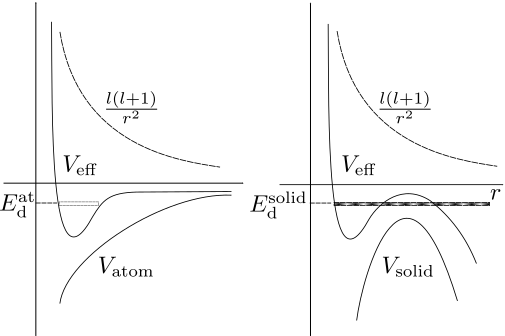
\includegraphics{./invariance/resonant-datoms.pdf}
\caption{The possibility of free electron states, in the interstitial region, 
resonating with atom centered localized states. The centrifugal components of the 
atomic d wave scattering channel can combine with
the atomic potential to produce a bound electronic state at some energy $E^{0}_{l}$ for an atomic system.
In a crystal the atomic periodic potential can be such that electrons can be bound in an
atomic d-like state can have the same energy as tunnel through the barrier localizing 
them and mix with free electron plane wave states. This dual character of the wave 
function, with localized components and extended components, requires careful 
detangling to return to a tight binding description. This difficulty 
stems from the presence of an energy resonance 
complicating the process of choosing the coefficients of the tight binding matrix. 
For the optimal, energy independent, set of coefficients that can be 
chosen see the work of Pettifor. There is a close parallel with the resonant
scattering of d-wave electrons in materials and Feshbach resonances Ref.~\cite{chin10}.
[Figure after D.W. Bullet Solid State Physics Vol. 35 pg. 197.]}
\end{figure}
%

From pseudopotentials we are familiar with having to match the logarithmic energy
derivative at some cutoff radius. Usually found by integrating the radial
Schr\"odinger equation to find $u_{l}(r,\epsilon)$ and matching the logarithmic derivatives:
%
\begin{equation}
L_{l}(\epsilon) \equiv \frac{u'_{l}(r_{0},\epsilon)}{u_{l}(r_{0},\epsilon)} = \frac{\kappa[j'_{l}
(\kappa r_{0}) - \tan \eta_{l} n'_{l}(\kappa r_{0})]} {j_{l}(\kappa r_{0}) - \tan \eta_{l} n_{l}'(\kappa r_{0})]},
\end{equation}
%
wherer:
%
\begin{equation}
\label{eq:phaseshift}
\tan \eta_{l} = \frac{\kappa j'_{l} - L_{l}j_{l}}{\kappa n'_{l} - L_{l}n_{l}}.
\end{equation}

In terms of the energy and width the l=2 phase shift Eq.~\ref{eq:phaseshift} 
can be written:
%
\begin{equation}
\label{eq:dshift}
\tan \eta_{d} = \frac{\frac{1}{2}W(\epsilon)}{\epsilon_{d}-\epsilon}.
\end{equation}
%
The uncertainty principle allows for the estimation of the rest
time for an electron on an atomic d state to be around $\hbar/W_{d}\approx 10^{-14}$s \cite{friedel73}.
\footnote{Ref.~\cite{friedel73}, written in 1973, provides us with another example
of the early impact electronic computers were making in the field. Friedel  compares 
the relative merits of `muffin tin' type calculations and tight binding approximations.
The former approach he describes as leading, ``to fairly exact if cumbersome
computations, and has thus had the support of the `computers lobby'". The conclusion
puts forward a number of points in favour of tight binding approaches as 
being suitable for studying complex phases and lattice defects,
latent heats of phase changes, elastic constants and electron-phonon couplings.}

The strong centrifugal contribution to the
atomic scattering potential from higher angular moment channels means the effective potential
can create a bound atomic state. In a solid the energy of this bound state can match the 
energy of a free electron state in the interstitial region and there will
be resonant tunneling between the two states. This results in the hybridization of d states
and plane waves. 

This means an appropriate model Hamiltonian must account for the various states as
%
\begin{align}
\label{eq:d-hamiltonian}
H =  d-d  |&  d-PW \\
     PW-D |& PW-PW 
\end{align}
%
where d-d and PW-PW are of the tight-binding and plane-wave 
pseudopotential form and hybridization occurring in the 
off-diagonal elements. The dual characteristic of transition metals
tightly bound d-electrons and diffuse s-p orbitals hybridizing 
accounts for the difficulties in describing their electronic properties.


The $dd\sigma$ terms behave roughly as \cite{pettifor71}:
%
\begin{equation}
\label{eq:pettifor}
dd\sigma \approx \frac{-5W\cos\kappa_{d}R}{\kappa_{d}R}
\end{equation}
%
If we write our basis functions in terms of localized orbitals
Eq.~\ref{eq:pettifor} suggests our Hamiltonian matrix will be 
populated by a huge number of off-diagonal matrix elements which can't be neglected. If 
the energy is equal to $k^{2}$ constructive interference occurs and the energy summation
diverges with off-diagonal matrix elements between all d states on remote atoms becoming
significant. This isn't entirely surprising. We are considering a periodic crystalline solid
and the eigenfunctions of this crystal are extended throughout. The off-diagonal elements
in a coordinate space representation reflect the long range order of the material and
preservation of the phase of the electronic wave function as they move from atom to atom. See
Chapter~\ref{chap:odlro} for further discussion of this and related points.

The `best' approximations to the explicit formulas for $dd\sigma$, $dd\pi$ and $dd\delta$ and the phase
shift $d_{0}'$ of the diagonal tight-binding elements 
These difficulty have been addressed in a number of works 
\cite{hubbard67,mueller67}, \cite{hubbard68}, \cite{hubbard69} \footnote{Another computational
snapshot comes from Ref.~\cite{hubbard69}, "...smaller secular 
equations are used, taking about one second per k point on an IBM  360/65." The
main storage capacity of those machines was 524 kilobytes. See Fig.~\ref{fig:ibm360}
for a (grainy) snapshot of what that computer looked like.},
and J. Hubbard, ibid 2, 1222 (1969). The problem being to define an
energy independent Hamiltonian, amenable to tight binding for the d electrons.

Deriving an effective, tight binding, energy indepedent parameterization
of d electron structure  culminated in the work of D. G. Pettifor's \cite{pettifor69}. 
Pettifor's work produced a justifiable scheme for computing the two center tight binding integrals of Slater
and Koster, $dd\sigma$, $dd\pi$, $dd\delta$ in terms of the position and halfwidth of the resonance:
$\epsilon_0$ and $\Gamma$. It is worthwhile considering the achievement of these collected papers.
With relatively limited computing power the workers determined 
the positions of atomic eigenvalues, band widths, and the effect 
of atomic scattering potentials. In 
the course of the work a great deal of algebraic manipulation of spherical 
harmonics and plane waves is required, along with the determination
of numerical values via graphical methods. All in all a laborious but fruitful task resulting
in energy independent matrix elements localized to nearest (next nearest ) 
neighbours real and reciprocal space.

The work of Pettifor and colleagues in determining justifiable tight 
binding parameters for transitional metals, 
effectively completed by 1969, was an important prerequisite for the subsequent 
development of the recursion method in the 1970s. Generalized tables for tightbinding parameters 
across the transition metal series has been produced in Ref.~\cite{harrison80}.

%The parameters used in Ref.~\cite{burke78} are appropriate to the BCC structure.
%The tightbinding Hamiltonian only considers two center contributions, with the parameters 
%coming from Pettifor\cite{pettifor69} and rescaled to produce the observed
%bandwidth of tungsten. The parameters are given in Table~\ref{tab:dsurface}.

For ease of reference we collect here d tight-binding coefficicents
that have found there way into the literature. The choice of these parameters
is very much an example of theoretical materials science constituting a 
craft. In later chapters we will examine some of the developments that set
tight-binding and the choice of coefficients on a more definite 
theoretical framework. The Slater-Koster parameters used for FCC, BCC, 
and HCP crystals in Ref.~\cite{haydock72} are given in Table \ref{tab:pettiparams}.
%
\begin{table}
\begin{center}
\begin{tabular}{|c|c|c|c|c|} 
\hline
Structure & $dd\sigma$ & $dd\pi$  & $dd\delta$ &  Band-limits \\
\hline
FCC       & -0.027784  & 0.012535 & -0.001554  & -0.131 to 0.085 \\ 
\hline
HCP       & -0.027784  & 0.012535 & -0.001554  & -0.119 to 0.081 \\
\hline
BCC       & -0.03248   & 0.01538  & -0.00200   & -0.119 to 0.097 \\
          & -0.01341   & 0.00487  & -0.00049   &              \\
\hline
\end{tabular}
\caption{Slater-Koster parameters from Pettifor \cite{pettifor69}, 
along with band edges in Ry. First and second nearest neighbour 
parameters are given for BCC crystals. \label{tab:pettiparams}.}
\end{center}
\end{table}
%
%\begin{table}
%\begin{tabular}{|c|c|c|}
%\hline
%SK Parameter & First Neighbour & Second Nearest Neighbour \\
%\hline
%$dd\sigma$ & -0.02992  & -0.05364 \\
%$dd\pi$    &  0.06652  &  0.01943 \\
%$dd\delta$ &  0.00800  &  0.00196 \\
%\hline
%\end{tabular}
%\caption{These parameters are difficult to make out from the electronic version of Ref.
%due to poor resolution of the scan. \label{tab:dsurface}.}
%\end{table}
%
\begin{table}
\begin{center}
\begin{tabular}{|c|c|c|}
\hline
\multicolumn{3}{|c|} {FCC TB Parameters} \\
\hline
Integral & 1st Nearest Neighbour & 2nd Nearest Neighbours \\
\hline
$dd\sigma$ & -0.027784 & - \\
$dd\pi$    &  0.012535 & - \\
$dd\delta$ & -0.001554 & - \\
\hline
\multicolumn{3}{|c|} {BCC TB Parameters} \\
\hline
Integral & 1st Nearest Neighbour & 2nd Nearest Neighbours \\
$dd\sigma$ & -0.06560  & -0.03195 \\
$dd\pi$    &  0.04373  & 0.02130\\
$dd\delta$ & -0.010934 & -0.00537\\
\hline
\end{tabular}
\caption{The tight binding parameters used for the example recursion 
calculations in this chapter, in the FCC lattice only nearest neighbours 
are included.}
\end{center}
\end{table}

Whether we are able to create a tight binding description of transition metals
depends on whether a decent, energy independent, approximation to the electronic 
structure in fcc/bcc metals can be achieved with 9x9 matrices describing 
nearest neighbour interactions of the s, p and d states, in the Slater-Koster 
form or derived from electronic states localized according to some 

\subsection{Kelly Tight Binding}

An example from Kelly helps to make the application of the tightbinding scheme clear:
%
\begin{quote}
As input data we require a convenient local representation of $H$. In simple crystals,
this is most easily given in terms of interactions with a unit cell and between neighboring cells.
For a FCC transition metal we have nine orbitals (1 s-orbital, 3 p-orbitals, and 5 d-orbitals) per site, 
and a diagonal 9x9 matrix for the self-energies of these orbitals. Twelve 9x9 matrices 
suffice to describe the interaction of any atom with its nearest neighbours.
\end{quote}
%

The actual operation of $H|u_{n}\ket$,which has been discussed in a general way so far, 
can be written as:
%
\begin{equation}
\label{eq:fullhamhop}
H|u_{n}\ket = \sum_{i\alpha, j\beta}a_{n i\alpha }(\bra j\beta |H| i\alpha \ket)|j \beta \ket.
\end{equation}
%
The summation in Eq.~\ref{eq:fullhamhop} does not run over every matrix element of the Hamiltonian.
Instead we appeal to the local formulation of the interactions so that
H can be stored and manipulated as a sparse matrix. To make this explicit let us 
introduce an index $z$ which runs over the nearest-neighbours of 
site $i$ with which the orbitals, $\alpha$, interact:
%
\begin{equation}
\label{eq:hop}
H|u_{n}\ket = \sum_{i\alpha, j_{z}\beta_{z}}a_{n i\alpha}(\bra j_{z}\beta_{z}|H_{z}|i\alpha\ket)|j_{z}\beta_{z}\ket.
\end{equation}
%
There are no restrictions on the number of orbitals per site, or on the range of interactions that can be
incorporated, these only impact on the efficiency of the method and the validity of the original assumptions
about the pre-dominance of the local atomic environment. Computationally Eq.~\ref{eq:hop} is at the
heart of all recursion calculations and the interested reader could at this point inspect the subroutine
\texttt{HOP} in \texttt{CamRecLib} to understand how the neighbour lists, matrix elements, and interaction
vectors are handled.

\section{Recursion Method}
The principle of the recursion method is to obtain a convergent expression 
for an element of the Green's function:
%
\begin{equation}
G(E) = \bra\phi_{i\alpha}|[E + i\delta -H]^{-1}|\phi_{i\alpha}\ket.
\end{equation}
%

The Green's function can be immediately related to the local density of states as:
%
\begin{equation}
n_{i\alpha}(E) = -\frac{1}{\pi} {\rm Im}\bra \phi_{i\alpha} |[E + i\delta -H]^{-1}|\phi_{i\alpha}\ket
\end{equation}
%

The state $\chi$ which we project on to can be made up of some linear combination 
of the local basis set $\phi_{\alpha l}$, which, in turn, could be local atom centered orbitals, bond orbitals, 
Wannier functions, atomic diplacements, or any localized quantity we wish to define. The method is thus
applicable to a wide range of problems in condensed matter. In short what we wish to examine
is determined by the choice of $\chi$.

\subsection{Mathematical Origin}
The trick of the recursion method, if you like to think of things in terms of tricks, 
or its generating feature, if you prefer, is that from the outset the `Greenian', the matrix element
of the Green's function we are interested in, is restricted to a particular matrix element: 
%
\begin{equation}
\label{eq:greenian}
G_{00}(E) = \bra u_{0}|[E-H]^{-1}|u_{0}\ket 
\end{equation}
%
As Heine puts it in his chapter:
%
\begin{quote}
Note that we do not want the whole of the inverse matrix $[E-H]^{-1}$, 
\emph{only one element}, and on this the whole method depends. In physics we do not
usually inquire about the whole of life, but about one particular matrix element (at a time) and we have chosen
$u_{0}$ so that Eq.~\ref{eq:greenian} gives us what, to put it crudely, we want.
\end{quote}

If we are given a tridiagonal matrix of the form:
%
\begin{equation}
H = \begin{bmatrix}
a_0 & b_1 & 0 & 0 & 0 &  ...\\
b_1 & a_1 & b_2 & 0 & 0 &  ...\\
0 & b_2 & a_2 & b_3 & 0 &  ...\\
0 & 0 & b_3 & a_3 & b_4 & ...\\
0 & 0 & 0 & b_4 & a_4 & ...  \\
0 & 0 & 0 & 0 & b_5 & ... 
\end{bmatrix}
\end{equation}

%
The determinants and sub-determinants of the matrix can be nested:
%
$$
\newcommand*{\temp}{\multicolumn{1}{|c|}{b_1}}
\newcommand*{\tempa}{\multicolumn{1}{|c|}{b_2}}
\newcommand*{\tempb}{\multicolumn{1}{|c|}{b_3}}
\newcommand*{\tempc}{\multicolumn{1}{|c}{0}}
\begin{array}{|ccccccc}
\cline{0-5}
a_0 & b_1 & 0 & 0 & 0 & 0  & D_0 \\ \cline{2-6} 
\temp & a_1 & b_2 & 0 & 0 & 0 & D_1 \\ \cline{3-6} 
0 & \tempa & a_2 & b_3 & 0 & 0 & D_2 \\ \cline{4-6}
0 & \tempc &  \tempb &  a_3 & b_4 & ... & D_3.
\end{array}
$$

Eq.~\ref{eq:greenian} can be rewritten in terms of its determinants:
%
\begin{equation}
\label{eq:greendet}
\bra u_{0}|[E-H]^{-1}|u_{0}\ket = \frac{{\rm det}|D_{1}|}{{\rm det}|D_{0}|},
\end{equation}
%
or, by flipping the fraction on its head:
%
\begin{equation}
\label{eq:greendet}
\bra u_{0}|[E-H]^{-1}|u_{0}\ket = \frac{1}{\frac{{\rm det}|D_{0}|}{{\rm det}|D_{1}|}}.
\end{equation}
%
Appeal is then made to Cauchy \index{Cauchy}\footnote{Baron Augustin-Louis Cauchy FRS FRSE (21 August 1789 – 23 May 1857)} 
for the following expansion:
%
\begin{equation}
\label{eq:cauchy}
{\rm det}|D_{0}| = (E-a_{0}){\rm det}|D_{1}|-b^{2}_{1}{\rm det}|D_{2}|
\end{equation}
%
and when generalized to determinants for $|D_{n}|$, $|D_{n+1}|$, and $|D_{n+2}|$:
%
\begin{equation}
\frac{{\rm det}|D_{n}|}{{\rm det}|D_{n+1}|} = E-a_{n}-\frac{b^{2}_{n+1}}{\frac{{\rm det}|D_{n+1}|}{{\rm det}|D_{n+2}|}}
\end{equation}

\footnote{
\index{C. Lanczos} J. Res. Natl. Bur. Stand. 45, 255 (1950) 
used the chain model in numerical work as a way of diagonalizing matrices
that could be implemented efficiently in a computer.
Chebyshev used chain models for approximating functions on an interval
P. L. Chebyshev, Bull. Acad. Imp. Sci. St. Petersbourg 1, 193 (1859)}

The coefficients of the continued fraction can be obtained from
a three term recurrence relation:
%
\begin{equation}
b_{n+1}|u_{n+1}\ket = H |u_{n}\ket - a_{n}|u_{n}\ket - b_{n}|u_{n-1}\ket
\end{equation}

where:
\begin{equation}
a_{n} = \bra u_{n}|H|u_{n} \ket,
\end{equation}
and 
\begin{equation}
b_{n} = \bra u_{n}|H|u_{n-1} \ket.
\end{equation}

This at least is the rationale given in Vol.~35. In the appendix we pursue an
alternative derivation of the recursion method that makes the connection
with some different mathematical techniques a little more explicit. For the connection
to tridiagonal matrices and expansions in terms of determinants
is good enough to satisfy our mathematical curiousity.

\section{Analytic Recursion}
\subsection{The Constant Chain}
The simplest chain model that can be handled analytically is the constant chain and it
serves as the paradigm of all the recursion calculations that will be undertaken. 
The constant chain corresponds to the general continued fraction written:
%
\begin{equation}
\label{eq:constantchain}
G_{0}(E) = \cfrac{1}{E-a_{0}-\cfrac{b_{1}^2}{E-a_{1}-\cfrac{b_{2}^{2}}{E-a_{2}-\cfrac{b_{3}^{2}}{...}}}},
\end{equation}
%
where $a_{0}=a_{1}=...=a_{n}=a$ and $b_{0}=b_{1}=...=b_{n}=b$. 
%
In this chain an electron experiences the same pull to 
every site on the chain, and can hop from one site to 
the next with the same hopping amplitude $b^{2}_{n}$. 
%
That all the coefficients are the same means a closed 
form solution can easily be found by recognizing that 
Eq.~\ref{eq:constantchain} can be written as:
%
\begin{equation}
G_{0}(E) = \frac{1}{E-a-b^{2}G_{0}(E)},
\end{equation}
%
and rearranged to give:
%
\begin{equation}
G_{0}(E) = (\frac{E-a}{2b^{2}}) \pm \sqrt{\frac{1}{4}(\frac{E-a}{b^{2}})^{2} - \frac{1}{b^{2}}}.
\end{equation}

The argument of the Green's function is $E + i\delta$, for positive 
energies the negative root is chosen and for negative energies 
the positive root is chosen. This gives the real
and imaginary part of the Green's function plotted 
in Fig.~\ref{fig:gfconstchain}.
%
\begin{figure}
\begin{center}
{\graphicspath{{./invariance/chain_figs/}}\input{./invariance/chain_figs/chain_plot.tex}}
\caption{Real and imaginary parts of the Green's function for the constant chain.\label{fig:gfconstchain}}
\end{center}
\end{figure}
%
The constant chain yields an analytic solution. All the coefficients of the continued
fraction are known and the recursion relation can be solved exactly. 

%In practice
%the computation of the $a_{n}$ and $b_{n}$ terms is truncated after some number.
%The function chosen to approximate the remaining coefficients is discussed in
%Refs.~\cite{haydock84, haydock85}.

A great deal of interesting physics can be obtained directly from the chain model. 
For instance, to couple an impurity to a constant chain we allow the first two coefficients $a_{0}$ and $b_{1}$ to vary, 
and the rest of the chain remains constant. This leads to the expression:
%
\begin{equation}
\label{eq:defectchain}
G(E) = \frac{1/b_{1}}{\frac{E-a_{0}}{b_{1}} - G_{0}(E)}.
\end{equation}
%
There are a few different cases depending on the relative magnitude of $a_0$ 
and $b_{1}$ and the chain parameters $a$ and $b$.
We plot the behaviour of the function for a few different choices of coupling parameters
$b_{1}$, and the relative position of the defect state $a_0$ in Fig.\ref{fig:gfdefect}. 
We will return to the idea of coupling single particle states to bands in Chap.~\ref{chap:manybodyrec}. 

In Fig.~\ref{fig:inband} the defect state energy is placed inside the energy range of the band. The
results for different couplings $b_{1}$ are plotted.
%
\begin{figure}
\begin{center}
{\graphicspath{{./invariance/chain_figs/}}\input{./invariance/chain_figs/inband_plot.tex}}
\caption{Defect chain model, Eq.~\ref{eq:defectchain}, with $a_{0}$ chosen to be 
within the band of energies for the constant chain. The strength of the coupling between the chain 
and the defect, $b_1$, is varied. For well matched systems the density of states splits 
into two resonances corresponding to bound and antibound states. \label{fig:impurity}}
\end{center}
\end{figure}
%

For $a_{0}$ outside the energy range of the band, the coupling to the band shifts the position
of the pole from $a_{0}$ and adjusts the areas under the two curves. Where there is 
near matching of the chain and the defect the function changes rapidly for small
variations in the coupling parameters.
%
\begin{figure}
\begin{center}
{\graphicspath{{./invariance/chain_figs/}}\input{./invariance/chain_figs/adsorbate_plot.tex}}
\caption{Coupling of an adsorbate to a constant chain model Eq.~\ref{eq:defectchain}. 
In this case $a_{0}$ is chosen to be outside the band formed by the chain.
Where there is strong coupling to the chain two distinct resonances appear.
The blue and green curves correspond to couplings of $b_{1}=2b$ and $b_{1}=b/10$ respectively.
\label{fig:gfconstchain}}
\end{center}
\end{figure}
%
In cases where the defect state is far removed and only weakly coupled to the band
there is only a small renormalization of the pole from $a_{0}$ and redistribution of the weight across the band.
This will be discussed more in Chap.\ref{chap:manybodyrec} in the context of single particle states
interacting with plasmon bands and the continuum.

\section{The Cambridge Recursion Library: \texttt {CamRecLib}}
Moving from analytic chain models to material systems with different atoms requires specification
of the Hamiltonian. The choice of the tight binding parameters was discussed in the first half of this
chapter. For present purposes the Slater-Koster tight binding parameters for the interaction of 
d-electrons should be sufficient to demonstrate the important features of typical recursion type calculation.
In subsequent chapters we will prefer the use of tight binding parameters based on Wannier functions.

\subsection{Integrals of the Density of States}
%
As will be seen, and is perhaps already known to the reader, nothing is perfect. The
recursion method for all its many strengths has an issue: the chain must be terminated
somewhere. In an extended system only so many moments can be computed in practice.  
This is not necessarily a defect of the method but a reflection of reality. Though
this is disappointing there is a silver lining. Integrals over the density of states
are very stable. As such any time we require an integral over the density of states
we can be quite confident in the result, similarly integrals over differences
are quite stable. This property of the recursion chains will be exploited again and again
to compute the relative stability of different structures. The details of how
integrals of continued fractions are performed is included in the appendix 
but it is highly recommended that the reader refer to Ref.~\cite{nex78}
for a formal description of the implemented techniques.

To compute the difference in energy between inequivalent structures 
one begins with the electron occupancy of a specific orbital:
%
\begin{equation}
N_{\alpha l}(E) = \int_{-\infty}^{E_{F}} n_{\alpha l}(E') dE'
\end{equation}
%

The total energy in a particular orbital:
%
\begin{equation}
U_{d} = \int_{-\infty}^{E_{F}}E'n_{\alpha l}(E') dE'
\end{equation}
%

The energy difference of two structures A and B can also be computed
to high accuracy:
%
\begin{eqnarray}
\label{eq:Ua}
U_{A} = \int_{-\infty}^{E_{FA}} E n_{A}(E) dE
\end{eqnarray}
%
\begin{eqnarray}
\label{eq:Ub}
U_{B} = \int_{-\infty}^{E_{FB}} E n_{B}(E) dE
\end{eqnarray}
%
\begin{equation}
\label{eq:totaldos}
Z = \int_{-\infty}^{E_{FA}} n_{A}(E)dE = \int_{-\infty}^{E_{FB}}n_{B}(E)dE
\end{equation}
%
\begin{equation}
U_{A}-ZE_{FA}= \int_{-\infty}^{E_{FA}}(E-E_{FA})n_{A}(E)dE
\end{equation}
%
\begin{equation}
U_{B}-ZE_{FA}= \int_{-\infty}^{E_{FA}}(E-E_{FA})n_{B}(E)dE + \int_{E_{FB}}^{E_{FA}}n_{B}(E)dE
\end{equation}
%
If $n_{B}(E)$ is taken to be constant across that small energy range, the second term, in
Eq. results in a small squared term that can be dropped. Swapping $E_{FB}$ and $E_{FA}$ gives
a similar result. This justifies dropping the A index on the Fermi energy to get the
final expression \cite{johannes76}:
%
\begin{equation}
U_{A}-U_{B} = \int_{-\infty}^{E_{F}}(E-E_{F})[n_{A}(E) -n_{B}(E)]dE.
\end{equation}
%

\subsection{Local Density of States}
\label{sec:fccldos}
The simplest demonstration of the Cambridge Recursion Library 
is a computation of the local density of states for an atom located at the center of a small 
Face Centered Cubic (FCC) cluster. 
Fig.~\ref{fig:cuboid} depicts a 75 atom cuboid cluster and the 
local density of states for an atom located in the middle of the cluster. 
The contribution of the electronic states to the total energy are also plotted. 
%
\begin{figure}
\begin{center}
\includegraphics[width=\columnwidth]{./invariance/rec_examples/exrecal/combined.png}
\caption{(a) 75 atom cuboid cluster of face centered cubic (FCC) crystal. Green 
atoms are in an FCC environment, and have a complete set of FCC neighbours, grey atoms 
are surface atoms of the cluster and a have a lower coordination number.
(b) Same cluster with an extra bulk atom and two additional atoms 
placed on the surface at two different sites. 
\label{fig:cuboid}}
\end{center}
\end{figure}
%
The density of states in Fig.~\ref{fig:fcc_dos} is computed by 11 iterations of the 
recurrence equation. This generates continued fraction coefficients
from $a_{0}$ to $a_{10}$ and $b_{0}$ to $b_{11}$. 
A basis of five d orbitals are chosen to reside on each atom 
and their interaction via the Hamiltonian is determined by the Slater-Koster parameters.
The Hamiltonian parameters and the coefficients of the continued fraction are given in Table~\ref{tab:reccoeffs}.
The total DOS in this case is computed by combining the continued fractions computed for each of the 
five starting orbitals into a single continued fraction 
(multiple sets of continued fraction coefficients can be combined via the 
routine \texttt{RECSUM} in \texttt{CamRecLib}). 
%
\begin{figure}
\begin{center}
{\graphicspath{{./invariance/rec_examples/exrecal/}}\input{./invariance/rec_examples/exrecal/recal_dos.tex}}
\caption{Top panel: the local density of states on the central atom for the FCC 
cluster in Fig.~\ref{fig:cuboid} is computed. 
Bottom panel:  The contribution of the band structure to the 
cohesive energy and the integrated density of states.\label{fig:fcc_dos}}
\end{center}
\end{figure}
%

\begin{table}
\begin{center}
\begin{tabular}{|c|c|}
\hline
$a_{n}$ & $b_{n}$ \\
\hline
 0.000000E+00 & 0.100000E+01\\
-0.736283E-02 & 0.295643E-02\\
-0.296524E-01 & 0.178593E-02\\
-0.126548E-01 & 0.221181E-02\\
-0.225989E-01 & 0.178256E-02\\
 0.296606E-02 & 0.141733E-02\\
-0.129493E-01 & 0.196435E-02\\
-0.136124E-01 & 0.141377E-02\\
-0.170328E-01 & 0.181703E-02\\
-0.161681E-01 & 0.173104E-02\\
 0.000000E+00 & 0.148088E-02\\
\hline
\end{tabular}
\caption{Coefficients for the continued fraction DOS for a $d_{xy}$ orbital of a Ni 
atom in the middle of a small nickel cluster.\label{tab:reccoeffs}}
\end{center}
\end{table}

The difference in the qualities, in terms of the structure revealed, in the DOS 
is determined by the size of the cluster, the number of iterations of the
recurrence relations, the Hamiltonian, and the different termination 
scheme employed. 
\footnote{See the routines \texttt{DENCRS} and \texttt{DENSQ} 
for the square root and analytic terminator (TermDOS) schemes and \texttt{DENQD} 
for the QuadDOS termination scheme in the Cambridge Recursion Library 
\cite{nex84,haydock84,haydock85}.
The asymptotic behaviour of the continued fraction coefficients 
are determined by the presence, nature and position of singularities
in the spectrum: band gaps, delta functions,
band edges themselves, and Van Hove singularities.
There is considerable literature on the topic of termination schemes 
and the analytic structure of the asymptotic coefficients:
\cite{hodges77,bylander80,turchi82,haydock84,luchini87,glanville88,
yoshino87,yoshino88,haydock89,haydock10,alhaidari18}.
In certain cases expressions for the behaviour of the coefficients
is given in terms of sinusoidal or elliptic functions. Linear prediction techniques
have also been used to study the behaviour of the recursion coefficients in the
asymptotic region \cite{allan84}. The problem of terminating the continued fraction
is quite an involved one and the discussion is deffered to the appendix.}

\subsection{\texttt{ORPEEL}: Orbital Peeling}
Surface catalysis is a topic of immense interest in chemistry and chemical engineering.
The rate at which reactions proceed is important in industrial and biomedical 
applications. The presence of a surface disrupts the periodicity required to use Bloch's theorem,
at least in the direction normal to the surface. In real systems
The periodicity parallel to the surface is also quite likely to 
be compromised by steps, terminating dislocation loops, 
vacancies and impurities. All this is to say that where 
there is a surface there is likely to be a need for recursion
techniques.

The need for a direct calculation of binding energy between adatoms or
the binding of a defect impurity in a lattice stems from the difficulties in computing 
these quantities via the method of energy differences. Performing two total
energy calculations on systems with on the order of $10^{23}$ atoms and subtracting the
resulting numbers is not a well conditioned problem. 
The very nature of the problem suggests that exploiting symmetries
will not greatly simplify things.

Relevant work on surfaces using the recursion method can be found in 
Refs.~\cite{haydock72, kelly73, kelly74, kelly74b, burke76, haydock79, haydock82}.
In particular \cite{haydock79} presents a quantitative treatment of chemisorption of simple
molecules to transition metal surfaces across the transition metal series. 
\footnote{This study provides a strong positive example of analysis of homologous 
trends in materials according to Ehrenreich's fourth point Chapter~\ref{chap:intro}}.
A detailed discussion of surface catalysis is also given in Ref.~\cite{haydock80}
for the dissociation of hydrogen on a transition metal surface. The apparent
connection to embrittlement phenomenon will be discussed in detail in Chap.~\ref{chap:metallurgy}.

The Cambridge Recursion Library provides an example 
to demonstrate some of the technique required to perform 
calculations of electronic properties on a surface. 

The example treats the problem of the interaction of adatoms on a 
surface, i.e. adatoms interacting via the metallic substrate.
The formalism was partially developed in Ref.~\cite{einstein73} and 
allowed for the study of adatom interaction energy 
as a function of the substrate band filling, adatom energy level, and the hopping
potential chosen between the adatom and the substrate. The generalization
to multiple orbital adatoms was given in Ref.~\cite{burke76}. 

The problem reduces to finding the difference in the total energy of the system when
adatoms are distant (infinitely separated) and when they are close together.
The total energy of the system is written:
%
\begin{equation}
U_{\rm TOT} = \sum_{i}\epsilon_{i} - U_{\rm ES},
\end{equation}
%
the first term is the band structure contribution to the energy, integrated
across all the occupied electronic states (on an adatom), and the second term is the electrostatic
energy, including the interelectron repulsion (to avoid double counting), and the repulsion
between the ion cores. It is the first term that is considered to be of primary 
interest in the example and corresponds to the energetic contribution coming 
from the adatoms sharing electrons via the d-band substrate.

The calculation proceeds as follows. First the two atoms are placed at a sufficient
distance that they do not interact and the energy:
%
\begin{equation}
U_{1} = \int_{-\infty}^{E^{(1)}_{F}}EN_{1}(E)dE,
\end{equation}
%
is computed. 

Then the two adatoms are allowed to come together on the surface, 
a new density of states is recalculated along with the new Fermi level.
%
\begin{equation}
U_{2} = \int_{-\infty}^{E^{(2)}_{F}}EN_{2}(E)dE,
\end{equation}

The integrals of the two density of states up to the two Fermi energies are equal
(no electrons have been added to the system).

The interaction energy can now be written:
%
\begin{equation}
W = \int_{-\infty}^{E_{F}} (E-E_{F})(N_{2}-N_{1}) dE
\end{equation}
%

The two reference systems are labeled System 1 and System 2. In Fig.~\ref{fig:burkesurf}
System 1 consists of two substrates each with an adatom, System 2 is a substrate with
2 adatoms and the empty substrate giving a Hamiltonian $H_{2}+H_{0}$.

The density of states then become:
%
\begin{equation}
N_{1} = 2{\rm Tr}[EI-H_{1}]^{-1}
\end{equation}
%
\begin{equation}
N_{2} = {\rm Tr}[EI-H_{2}]^{-1}
\end{equation}

Finally the identity: 
%
\begin{equation}
{\rm Tr}[EI-H]^{-1} = \frac{\partial}{\partial E} \log \det[EI-H],
\end{equation}
%
is employed to reach an expression for the difference in the density
of states $\delta N=(N_{2}-N_{1})$.
%
\begin{equation}
\delta N = \frac{\partial}{\partial E}\log\frac{\det[EI-H_{2}]}{\det [EI-H_{1}]}\frac{[EI-H_{0}]}{[EI-H_{1}]}
\end{equation}
%

What then follows is some consideration of the block structure of the matrices 
$H_2$, $H_1$ and $H_0$. $H_2$ is a partitioned matrix of dimension 
$5N+6$ and $H_1$ has dimension $5N+3$. $H_{0}$ is the substrate Hamiltonian 
with dimensions $5\times N$ (orbitals times atoms).
The self energy elements are given in the block $E_A$, $V_{1}$ and $V_{2}$ describe
the atoms interactions with the substrate and the $V_{12}$ describe the interaction
between adatoms. Some identities from matrix algebra employed in Ref.~\cite{einstein73}
and given in the appendix of Ref.~\cite{burke76} are then used to simplify the
expressions to:
%
\begin{equation}
\delta N = \frac{\partial}{\partial E}\log \frac{\det G_{1}}{\det G_{2}}
\end{equation}
%

The physical meaning is that $\log \det G_{2}$ gives the energy required to pull
one of two adatoms away from the substrate and its paired atom, the $\log \det G_1$
term is the energy required to put it back on substrate at an isolated site. 
The difference between these two energies is then the interaction energy. 
Formulating the problem as a matrix means the determinant can be split 
into a sum over five separate logarithms. This is accomplished by ``orbital peeling".

\begin{equation}
{\rm det}|G_{2}| = \bar{G}_{21}\bar{G}_{22}\bar{G}_{23}\bar{G}_{24}\bar{G}_{25}
\end{equation}

\begin{equation}
{\rm det}|G_{1}| = \bar{G}_{11}\bar{G}_{12}\bar{G}_{13}\bar{G}_{14}\bar{G}_{15}
\end{equation}

The matrix elements for each $G_{i\alpha}$ should be very familiar at this point:
%
\begin{equation}
G_{i\alpha}=\bra i,\alpha| [E-\bar{H}_{i\alpha}]^{-1} |i, \alpha\ket
\end{equation}
%
with $i=1,2$ $\alpha=1,5$. The matrix $\bar{H}_{i\alpha}$ is formed by taking 
$[E-\bar{H}_{i}]$, deleting the first $(\alpha-1)$ rows and columns 
to form $[EI-\bar{H}_{i\alpha}]$. The desired matrix element is now 
in the upper left-most corner of the matrix. 
Using this representation the difference in the density of states is calculated:
%
\begin{equation}
\Delta N = \sum_{\alpha=1}^{5} \frac{\partial}{\partial E}(\log\bar{G}_{1\alpha} - \log \bar{G}_{2\alpha})
\end{equation}
%

%
%The range of $E_{F}$ is restricted to $-0.068 \ge E_{F} \le 0.12$ Ryd by considerations
%based on the atomic configuration of tungsten as $5d^{4}6s^{2}$, meaning the band 
%should contain a minimum of 4 and a maximum of 6 electrons, with the band being half filled (5 e)
%considered the most plausible.

Fig.~\ref{fig:burkesurface} shows the energy difference as a function of the 
Fermi energy position. The energy is computed from the three p orbitals of a 
surface atom adhered to the same cluster studied in Sec.~\ref{sec:fccldos}.
%
\begin{figure}
\begin{center}
{\graphicspath{{./invariance/rec_examples/exorpeel/}}\input{./invariance/rec_examples/exorpeel/exorpeel.tex}}
\caption{Top panel: Adsorbate interaction energy as a function of the Fermi energy for a representative d band
substrate. Mutual interaction of the adsorbates is mediated by the substrate and the p-d surface interaction.
Interaction goes to zero when the substrate band is completely filled. 
Bottom panel: Difference in the total energy for the two adsorbate configurations as a function of
d-band filling (position of the Fermi energy). See Ref.~\cite{burke76} for details. \label{fig:burkesurface}}
\end{center}
\end{figure}
%

These early surface calculations using the recursion method were overwhelmed 
by a number of uncertainties. The lack of a procedure for a choice of the tight-binding 
Hamiltonian and difficulties in accessing the self consistent charge density
and relaxed configurations in the presence of a surface being the most significant.
\footnote{For early work on Wannier functions at surfaces Ref.~\cite{smith74}. Also see 
\cite{mostoller79} for a treatment of surface effects using the recursion method.}

The development of first principles calculations 
has greatly simplified access to these quantities and should remove 
some of the ambiguities in mapping ab initio data onto a local picture
of the electronic structure at surfaces. These advances mean that the 
recursion techniques described in Refs.~\cite{burke76, haydock79, haydock81} 
might be revisited with potentially profitable effect. 

The interactions and forces of atoms adhered to surfaces are directly 
observable experimentally see Fink~\cite{fink84}.
For applications of orbital peeling to defects and the 
computation of interaction energies and variations in the charge density
see Refs.\cite{gibson93,gibson94}. However that work partially relies 
on the computation of off diagonal of the Green's function. A topic
to which we turn now.

\subsection{Off-Diagonal Elements of the Green's Function}
The off-diagonal elements of the Green's function can be written:
%
\begin{equation}
G_{AB}(E) = \bra \phi_{A}|[H-E]^{-1}|\phi_{B}\ket,
\end{equation}
%
and they contain a lot of useful information. 

These off-diagonal elements are required to calculate 
response functions, \cite{terakura78}, interatomic 
forces \cite{finnis84, finnis87, ohta87}, and bond orders 
\cite{coulson39,tersoff86,pettifor89}.

One direct route to computing an off-diagonal elements of the Green's function
is by expressing it as a linear combination of two diagonal elements. 
This can be seen by forming new starting vectors 
from the potential linear combinations of $\phi_{A}$ and $\phi_{B}$:
%
\begin{align}
\phi_{+} = \frac{1}{\sqrt{2}}(\phi_{A} + \phi_{B})\\
\phi_{-} = \frac{1}{\sqrt{2}}(\phi_{A} - \phi_{B})\\
\phi_{i+} = \frac{1}{\sqrt{2}}(\phi_{A} + i\phi_{B})\\
\phi_{i-} = \frac{1}{\sqrt{2}}(\phi_{A} - i\phi_{B}),
\end{align}
%
we can retrieve the off-diagonal elements by computing 
two `normal' diagonal elements from these linear combinations.
For example, for an Hermitian $\hat{H}$, and real $\phi_{A}$ and $\phi_{B}$ 
the $AB$ off-diagonal element of the Green's function can be computed as:
%
\begin{equation}
\label{eq:offdiaggreen}
G_{AB}(E) = \frac{1}{2}[G_{++}(E)-G_{--}(E)].
\end{equation}

\subsection{The Tight Binding Bond Model}
\label{sec:tbbm}
To see how the off-diagonal elements contribute to the force on an 
atom we follow Sec. 2.4 of Sutton \cite{sutton88} and Ohta \cite{ohta87}.
First we reproduce their expression for the bond energy:
%
\begin{equation}
\label{eq:tbenergy}
u_{ij} = u^{\rm rep}_{ij} - \frac{4}{\pi}\sum_{\lambda\mu} 
h_{ij}^{\lambda\mu}{\rm Im}\int_{-\infty}^{\epsilon_{F}}G_{ji}^{\mu\lambda}(\epsilon+i0)d\epsilon,
\end{equation}
%
The total energy is then a sum over the bond energies:
%
\begin{equation}
\label{eq:tbtoten}
U^{\rm tot} = \frac{1}{2}\sum_{ij,(i\neq=j)}u^{\rm tot}_{ij}
\end{equation}
%

The expression for the bond force follows naturally as the gradient of the bond energy:
%
\begin{equation}
\label{eq:tbforce}
f_{ij}^{\alpha} = f^{\rm rep}_{ij\alpha} - \frac{4}{\pi}\sum_{\lambda\mu} 
\nabla_{i\alpha}h_{ij}^{\lambda\mu}{\rm Im}\int_{-\infty}^{\epsilon_{F}}G_{ji}^{\mu\lambda}(\epsilon+i0)d\epsilon,
\end{equation}
%
$\alpha$ is a Cartesian direction, $i,j$ are site indices, and $\lambda, \mu$ are orbital indices 
the z axis lies along the bond connecting atoms i and j. 
We will return to the first term in Eq.~\ref{eq:tbforce} in Sec.~\ref{sec:harrisfoulkes} 
and Chapter~\ref{chap:wannier}. The computation of the derivative
of the Slater-Koster matrix elements, $\nabla h_{ij}^{\lambda\mu}$,
is discussed in Appendix~\ref{appen:grouptheory}.

For now it is the second term that is of interest and
it is easily recognized as something we can access via the Green's function 
computed using recursion techniques. It is also important to note that 
Eq.~\ref{eq:tbforce} is certainly not a two body interaction! The Green's function 
as it is calculated accounts for information from every shell of neighbours 
until there are no more or the recursion process is terminated. 
The importance of this local formulation of forces should not be underestimated.
Many of the practical applications discussed in Chapter~\ref{chap:metallurgy} 
will rely on it.

%
These off-diagonal elements are also required to determine the vibrational properties. 
If we want the interatomic force constants determining the harmonic energy surface 
we follow Finnis\cite{finnis84} and go to second order in the variation of the 
total energy to derive the interatomic force constant matrix:
%
\begin{equation}
\label{eq:tbdynmat}
\psi_{\alpha\beta}^{ab} = \hat{\psi}_{\alpha\beta}^{ab} +  \sum_{dnq\sigma}(\delta 
\rho_{bd,a\alpha}^{nq,\sigma}\nabla_{\beta}h_{db}^{qn} + \delta\rho_{ad,b\beta}^{nq,\sigma}\nabla_{\alpha}h_{da}^{qn}),
\end{equation}
%
$h^{qn}_{db}$ is a two center hopping integral that links the orbital n on atom b to orbital 
q on atom d. For the d electrons this integral is taken to decay as
$\r^{5}$. The density changes are proportional to the variation in the Hamiltonian 
multiplied by the response function. Displacing atom a in the $\alpha$ direction induces a change in the
bond charges about atom b. The change in the bond charge between atoms b and d 
in the spin-$\sigma$ channel stemming from orbitals n and q is then given by:
%
\begin{equation}
\label{eq:tbdeltarho}
\delta \rho_{bd,a\alpha}^{nq,\sigma} = \sum_{cmp}(\chi_{bc,ad}^{np,mq,\sigma}+\chi_{ba,cd}^{nm,pq,\sigma})\nabla_{\alpha}h_{ac}^{pm}
\end{equation}
%
where the response function is defined as:
%
\begin{equation}
\label{eq:tbresponse}
\chi_{bc,ad}^{np,mq,\sigma} = \frac{1}{\pi}{\rm Im}\int^{E_{F}}G_{bc}^{np,\sigma}(\epsilon)G_{ad}^{mq,\sigma}(\epsilon)d\epsilon,
\end{equation}
%

An interesting relationship can be derived between off-diagonal elements
and the response functions \cite{terakura82, sutton88}:
%
\begin{equation}
\frac{dG}{dE}=-G^{2},
\end{equation}
%
and upon integration:
%
\begin{equation}
G_{jk}(E^{+}) = -{\rm Im}\int^{E}\sum_{l}G_{jl}(E')G_{lk}(E')dE'.
\end{equation}
%

Fig.~\ref{fig:tbresponse} gives a pictorial representation of some of these many indiced terms. In 
Ref.\cite{finnis84} the Green's functions are computed out to sixth nearest neighbour. This allows
for force contributions out to the thirteenth nearest neighbour. Symmetry relations are exploited 
in that work to reduce the number of unique off-diagonal Green's function elements to 
33 separate functions which are tabulated and used to compute the force constant matrix. 
%
\begin{figure}
\begin{center}
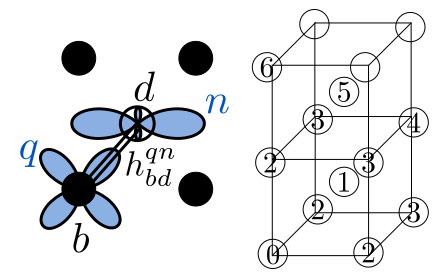
\includegraphics[scale=0.8]{./invariance/tbresponse.pdf}
\caption{Pictorial representation of the terms and sites 
described by Eq.~\ref{eq:tbdynmat}. On the left atoms $b,d$ 
and two orbitals centered on those sites, $n, q$, and the energy
integral $h_{bd}^{qn}$ which connects them. On the right are two unit cells
of BCC crystal with the nearest neighbours to the zeroth atom 
labeled out to its sixth nearest neighbour.\label{fig:tbresponse}}
\end{center}
\end{figure}

The type of analysis in Ref.~\cite{finnis84} is taken as an example
of the desired computational framework these notes pursue. 
The approach satisfies many of Ehrenreich's points ~\ref{en:ehrenreich}: 
direct experimental links, tractable calculations 
for a minimally idealized system, and, most importantly, 
the calculations have {\emph explanatory and predictive power 
across a homologous series}, in this case the BCC transition metals.
\footnote{For neutron spectroscopy data determining vibrational modes 
see \cite{powell68, colella70, shaw71}, The mystery of obtaining a 
good experimental phonon spectra in published literature continues... 
A. M. B. G. De Vallera, Ph.D. thesis, Cambridge University, 1977 (unpublished).
However it is apparently quite similar to NbMo\cite{powerll68}.}

The only point not fully satisfied is that of theoretical justification.
The force constants as determined in Eq.~\ref{eq:tbdynmat}
rely on the repulsive force and some means of determining 
the local Hamiltonian i.e. its bond integrals and their 
radial dependence {\it ab initio}. Addressing these issues
will be the subject of subsequent chapters. 
 
Eqs.~\ref{eq:tbdynmat, eq:tbdeltarho, eq:tbresponse} encode
a huge amount of information. Although well developed reciprocal space 
techniques exist, see Ref.~\cite{baroni01}, to obtain the phonon dispersion
curves, the local formulation still has a great deal of 
interprative value, and crucially, will remain valid
in situations where Bloch's theorem does not.

\section{The Bond Order}
\index{bond order}
The concept of a bond order has a long history.
It begins with Coulson's study of polyenes and aromatic 
molecules \cite{coulson39,coulson47}. Coulson's definition 
of the bond order begins from a molecular orbital picture. The molecular
orbital is a linear combination of atom centered orbitals $\psi_{n}$:
%
\begin{equation} 
\Psi = a_1\psi_1 + a_2\psi_{2} + ... +a_{n}\psi_{n},
\end{equation}
%
where $\sum_{n} a^{*}_{n}a_{n} = 1$, in Coulson's notation the bond order
then becomes:
%
\begin{equation}
\Theta_{ij}  = \frac{1}{2}[a_{i}a^{*}_{j} + a^{*}_{i}a_{j}].
\end{equation}
%
(where we have changed the notation of the bond order to the greek capital
theta rather than Coulson's preferred $p_{ij}$).
He goes on to examine the bond order in benzene, cyclobutadiene, 
and the alkyl chains C$_{\rm 2n}$H$_{\rm 2n+2}$ and alkyl radical chains 
$C_{2n+1}H_{2n+3}$ see Fig.~\ref{fig:coulsonmolecules}. 

The case of a hydrogen molecule $H_{2}$ is the simplest to 
visualize (panel Fig.~\ref{coulsonmolecules}). We build a wave function:
%
\begin{equation}
\Psi = \frac{1}{\sqrt 2}(\psi_{1} \pm \psi_{2})
\end{equation}
%
and the bond order is $\Theta_{ij} = \pm \frac{1}{2}$.

We may also consider $H_{2}^{+}$ and build a wave function:
%
\begin{equation}
\Theta_{ij} = \frac{\lambda\psi_{1} + \mu\psi_{2}}{(\lambda^{2} + \mu^{2})^{\frac{1}{2}}},
\end{equation}
%
the bond order is maximized when $\lambda=\mu$, the two nuclei share the 
single electron equally. 

As a second example imagine a benzene molecule and we have a nearest neighbour 
hopping integral of $\beta$ (neglect any overlap of the orbitals).
We can build up the following molecular orbitals:
%
\begin{align}
\psi^{(1)} = \frac{1}{\sqrt{6}}[\psi_{1} +\psi_{2} +\psi_{3} + \psi_{4} + \psi_{5} + \psi_{6}],\quad \epsilon=-2\beta\\
\psi^{(2)} = \frac{1}{\sqrt{6}}[\psi_{1} + w\psi_{2} + w^2\psi_{3} + w^3\psi_{4} + w^4\psi_{5} + w^5\psi_{6}],\quad \epsilon=-\beta\\
\psi^{(3)} = \frac{1}{\sqrt{6}}[\psi_{1} + w^5\psi_{2} +w^4\psi_{3} + w^3\psi_{4} + w^2\psi_{5} + w\psi_{6}]\quad \epsilon=-\beta
\end{align}
%
the factor of $w=e^{\frac{i\pi}{3}}$, i.e. the roots of unity, ensures we have a normalized wavefunction. 
From the coefficient of the wavefunction the bond order can be computed directly and the total energy,
what Coulson calls the total ``mobile energy", but what would be called the band energy today is
given by:
%
\begin{equation}
\epsilon = -2\sum_{ij}\Theta_{ij}\beta_{ij}
\end{equation}
%
\begin{figure}
\begin{center}
\includegraphics[scale=1.0]{./invariance/coulsonbondorders.png}
\caption{An intuitive picture of the bond order can 
be grasped by considering some simple molecules: (a) H$_{2}$,
(b), cyclobutadiene, (c) benzene, and (d) alkyl radicals.
Coulson was able to make convincing quantitative 
arguments about the variation of the bond lengths and energetics
in these types of systems from the point of view of the bond order. 
\label{fig:coulsonmolecules}}
\end{center}
\end{figure}

Coulson's correlation of experimental data in the form of bond lengths
with the concept of the bond order in polyenes and aromatic molecules
is an elegant demonstration of a theory and application closely
linked to experimental data, and studying trends in a class of
homologous materials. A very deep understanding of the energetics of 
hydrocarbon chains is made.

The bond order quantifies the accumulation or depletion of charge between
atoms as the coefficients of the orbitals are tuned to minimize the total energy.
Coupled with Feynman's intuition of positive nuclei being attracted to regions
of accumulated negative charge we begin to understand how solids are held together\cite{feynman39}.
It is of further interest to note that Coulson's paper requires the calculation of 
the determinate for a tridiagonal Hamiltonian (see also Ref.~\cite{coulson38}). 
The mathematics involved will be familiar to those happy students 
who have studied the linear chain model.

\footnote{Altmann and Bowens biographical sketch of C.A.Coulson\cite{altmann74} 
is highly recommended reading. As a contemporary of Dirac at Cambridge
Coulson witnessed first hand the early developments of quantum theory.\index{Coulson, C.A.} 
He would go on to play an early role in the application of wave mechanics 
to the study of molecules and crystals. 
In fact, Coulson is supposed to have attended a seminar given by Dirac 
where Dirac was discussing the uncertainty relation: $xp-px=ih$.
When Coulson inquired when this work had been done Dirac replied, 
``Last night." In 1938 Coulson may have performed what was
the first iterative self-consistent field calculation
on a molecule, H$_2$, by hand (with the possible help of a 
Brunsviga calculator purchased for \pounds 25.)
~\cite{coulson38}. Coulson's life work spans diverse fields.
A small selection from his bibliography will find work 
touching on numerical methods \cite{coulson37,coulson42}, 
random walks with an application to a certain type of slug 
traversing a surface in the presence of a bright light \cite{coulson47}, 
the electronic structure of aromatic compounds and polymers, 
dielectric media, and theology. The application of the methods 
reviewed in the present work to his fields of endeavour would 
constitute a textbook onto itself.}

The order of a given bond is a measure
of the force tending to change the length of a given bond
for a small variation of the bond length.

Defined in terms of Green's functions, the bond order is the integrated 
energy difference between a symmetric and anti-symmetric combination 
of nearest neighbour orbitals \cite{pettifor89}:
%
\begin{equation}
\label{eq:bondorder}
\Theta_{ij} = - \frac{2}{\pi} {\rm Im} \int^{E_{F}}\left[G^{+}_{00}(E)-G_{00}^{-}(E)\right]dE.
\end{equation}
%
The bond order in this form then appears like a measure of the interference 
between orbitals on the two sites.

As we integrate up in energy the difference in the symmetric and antisymmetric 
combinations of the two states are accumulated. The resulting integral is 
then a scalar which measures the sign and magnitude of the
interference between the two localized orbitals up to the Fermi energy.

Eq.~\ref{eq:offdiaggreen} gives an immediate scheme for computing the 
off-diagonal elements but can result in the need for substracting 
two largish quantities to find a small one. Such a procedure 
is never ideal. This concern and others motivated the introduction
of the block recursion method which will be discussed shortly.

First though a small digression.

Harrison in his textbook argues that every conclusion drawn in 
his work follows immediately from the proposition that electrons 
are simultaneously a particle and a wave. 
In the context of the recursion method we can propose 
a tentative meaning to his statement: the electron is a 
particle when we can point to it and say, `There it is. 
It is in that orbital centered on that atom.' It becomes a wave 
when the recursion process is initiated and the spectral weight of the 
localized orbital spreads outwards onto neighbouring atoms. 
The form this interaction takes in the recursion method 
is the linear mixing of the starting vector
with the other localised vectors in the system from 
further and further away, adding these vectors with changing coefficients,
allowing them to interfere constructively or deconstructively. 

When the recurrence is terminated a record of the projection of 
the starting orbital on to each of its increasingly distant neighbours 
is recorded. The electron, though confined to a discrete energy 
and state on the lone atom, when placed in a solid, can 
take on a range of shapes across a range of energies distributed 
throughout a crystal.

\subsection{Non-Orthogonal Recursion}
\label{sec:tensornotation}
The underlying assumption about the basis vectors
used to describe the system up to this point have 
been that they are orthogonal. However the most intuitive basis set to 
choose, a basis of atomic orbitals centered on an atom, 
the original choice made by Bl\"och, will not be orthogonal. 

L\"owdin functions are a class of localized orthogonal functions,
as are Wannier functions but the price to be paid for
obtaining these functions is often that of an entire 
first principles calculation. These matters will 
be discussed further in Chap.~\ref{chap:wannier}.

Anderson's chemical pseudopotential theory is formulated 
in terms of a generalized eigenvalue problem \cite{anderson68,anderson69}
as are the molecular building block type orbitals of \cite{edmiston63} 
and the work of Boys and Boys and Foster~\cite{boys60a,boys60b}. 

Though we begin to digress it is clear that for physical 
and numerical accuracy we require an orthogonal basis 
set but for intuition or heuristic purposes we may wish to continue thinking
in terms of nicely formed localized starting states that 
are not orthogonal but easy to picture and initialize.

In any case when the basis vectors set up to describe the system
are not orthogonal some choices need to be made. There are two options.
The most tempting option is just to ignore the non-orthogonality of the
vectors and carry on. The other is to modify our approach somewhat. 
The latter course is the morally upright one. 

If the basis set for the Hamiltonian is given as a set of
${\phi_{m}}$ orbitals elements of the overlap matrix can 
be written:
%
\begin{equation}
[S]_{mn} = \int \phi^{*}_{m}(\r)\phi_{n}(\r)d\tau
\end{equation}
%

Given two states $\mathbf{u}$ and $\mathbf{v}$ which
are linear combinations of the $\phi$ the physical
overlap of the states is given: $\mathbf{v}^{\dagger}S\mathbf{u}$.

The Hamiltonian operator $\mathcal{H}$ acts on a basis orbital and
its effect is approximated by a sum over the basis orbitals:

\begin{equation}
\mathcal{H}\phi_{n}(\mathbf{r}) = \sum_{n=0}^{\infty} H_{mn}\phi_{m}(\r)
\end{equation}

If the basis set is not orthogonal the Hamiltonian operator
is related to its representation in the basis set as:

\begin{equation}
\mathcal{H}_{mn} = [SH]_{mn}
\end{equation}

In the cases where S and $[\mathcal{H}_{mn}]$ are known the Hamiltonian
matrix is required which is obtained from:
%
\begin{equation}
H = S^{-1}[\mathcal{H}_{mn}],
\end{equation}
%
this transformed matrix is sometimes denoted $D$ in the literature
see Ref.~\cite{weeks73} for a discussion of the properties of
this transformed Hamiltonian. S should hopefully have some 
nice properties like its diagonal elements are unity and that it 
possesses small off-diagonal elements that fall off relatively 
quickly in real space.

The previous notation follows Haydock's article in Vol. 35 and uses 
a calligraphic $\mathcal{H}$ to denote the Hamiltonian operator and 
a roman $H$ with subscripts to denote the matrix elements of this operator 
projected onto the chosen basis set. 

In Ref.~\cite{ballentine86} Ballentine and Kol\'a\'r introduced 
a compact tensor notation to keep track of whether one was working 
with matrix elements of the overlap matrix and Hamiltonian 
in the non-orthogonal basis or in the Hamiltonian transformed by
the overlap matrix. The call to follow this tensor notation 
was echoed in Ref.~\cite{sutton88} and we describe it here to help
clarify the implementation of the non-orthogonal recursion method.
In Ref.~\cite{foulkes86} this notation was exploited in order to 
study some extensions of the recursion method to the evaluation of 
operator matrix elements. A transparent notation can greatly clarify
the concepts.

In what follows the lower case greek letters in the sub and superscripts
denote a composite orbital index comprised of the site-index and the 
angular momentum channel. In later sections of this chapter this notation
might be expanded with site indices denoted using lower case
roman letters and orbital indices denoted by lower case greek letters.
An effort is made to use $\alpha$ and $\beta$ where the index is a composite
one and $\lambda$, $\mu$, where they refer only to orbital indices with the 
site index made explicit. The usage should be clear from the context.

The matrix element of the overlap between non-orthogonal 
basis functions can be written:
%
\begin{equation}
S_{i\alpha j\beta} = \bra \psi_{i\alpha}|\psi_{j\beta}\ket
\end{equation}
%
with $i,j$ referring to a site index and $\alpha$ and $\beta$ 
referring to orbital indices.

The matrix elements of the Hamiltonian with the non-orthogonal states takes
the form:
%
\begin{equation}
H_{i\alpha j\beta} = \bra \psi_{i\alpha}|H|\psi_{j\beta}\ket
\end{equation}

The inverse of the overlap matrix is defined:
%
\begin{equation}
\sum_{j\beta}(S^{-1})^{i\alpha j\beta}S_{j\beta l\gamma}=\delta^{i\alpha}\ _{l\gamma}.
\end{equation}
%

Naturally, the elements of the inverse overlap matrix $S^{-1}$ are chosen 
such that they produce the identity matrix upon multiplication $S$.

The dual set of basis vectors are then:
%
\begin{equation}
|\psi^{i\alpha}\ket = \sum_{j\beta}|\psi_{j\beta}\ket(S^{-1})^{j\beta i\alpha}.
\end{equation}
%
If the overlap matrix is just the identity matrix the original 
basis set is already orthonormal and the dual vectors (covariant
contravariant, or upper and lower indiced, depending
on your naming preference) are equal.

The two most important aspects of any basis set
are {\it representation} and {\it normalization}. 
We can {\it represent} an arbitrary physical 
vector $|u\ket$ as:
%
\begin{equation}
|u\ket = \sum_{i\alpha}u^{i\alpha}|\psi_{i\alpha}\ket = \sum_{i\alpha}u_{i\alpha}|\psi^{i\alpha}\ket.
\end{equation}
%
The expansion coefficients in either basis can be obtained via:
%
\begin{equation}
u_{i\alpha} = \sum_{j\beta}S_{i\alpha j\beta}u^{j\beta}.
\end{equation}
%

Along with {\it representation} we require a {\it norm} i.e. 
the inner product of two vectors:
%
\begin{equation}
\bra v|u \ket = \sum_{i\alpha i\beta}v^{i\alpha *}S_{i\alpha j\beta}u^{j\beta} = \sum_{i\alpha}v^{i\alpha *}u_{i\alpha} 
= \sum_{j\beta}v_{j\beta *}u^{j\beta}
\end{equation}
%

The Hamiltonian in a mixed representation takes the form:
%
\begin{equation}
\label{eq:mixedH}
H^{i\alpha}\ _{j\beta} = \sum_{\gamma}(S^{-1})^{i\alpha k\gamma}H_{k\gamma j\beta}.
\end{equation}
%
In the literature this form of the Hamiltonian matrix is sometimes referred to as $D$ 
not to be confused with $D$ as it applies to the force constant matrix in Ref.~\cite{weeks73}
and Sec.~\ref{sec:recphonon}.

The reason for going to all this trouble of defining upper and lower
indexed vectors and a tensor notation is illustrated by considering how the Schr\"odinger
equation looks in different representations. If one works with
the easily instantiated, in the sense that one has the Hamiltonian and
overlap matrix elements to hand, but non-orthogonal basis set, then the Schr\"odinger
equation takes the form:
%
\begin{equation}
H..\psi^{\mbox{\large .}}=\epsilon S..\psi^{\mbox{\large .}}
\end{equation}
%

However if the Hamiltonian is converted to the mixed representation:
%
\begin{equation}
H^{\mbox{\large .}}.\psi^{\mbox{\large .}}=\epsilon\psi^{\mbox{\large .}}
\end{equation}
%
the overlap matrix disappears and the eigenvalue problem is in a 
more familiar form. The Hamiltonian in the mixed representation 
is that obtained from Eq.~\ref{eq:mixedH}. The price is the Hamiltonian
is no longer necessarily Hermitian and the overlap matrix has to be inverted.

The starting vector for the recursion will often be a lower indiced
vector corresponding with the basis set chosen to represent the electron
states.

Ballentine and Koclar conclude by giving the trace of an operator
(roman site indices are suppressed):
\begin{align}
{\rm Tr}A =& \sum_{\alpha\beta}S_{\alpha\beta}A^{\beta\alpha}\\
          =& \sum_{\alpha\beta}(S^{-1})^{\alpha\beta}A_{\beta\alpha} \\
          =& \sum_{\alpha}A^{\alpha}\ _{\alpha}
\end{align}

The trace of the Hamiltonian or density operator would be necessary 
if one wished to compute, for example, the total band energy 
or the charge density. Computationally the way of proceeding will
depending on which matrix elements one has to hand, 
the lower indiced being the more accessible generally. 

As mentioned the trouble with the mixed representation of the Hamiltonian is,
although it escapes the need to deal directly with the overlap 
matrix or its inverse, it is no longer Hermitian. 

The following two subsections suggest a generalization of the recursion
scheme to deal with non-Hermitian matrices, and a practical means
of performing non-orthogonal calculations which exploit the Gauss-Seidel
iterative scheme to obtain the inverse of the overlap matrix.
In effect these two approaches amount to the choice of working
in the mixed representation or working with the inverse of the overlap
matrix and the lower indiced Hamiltonian respectively.

\subsubsection{Two-Sided Lanczos}
For the case where $H\neq H^{\dagger}$, i.e. for a non-Hermitian
Hamiltonian, a two-sided Lanczos algorithm exists as discussed in
Ref.\cite{haydockkelly75} following Wilkinson's description.

Two starting vectors are chosen $|u_{0}\ket=|0\ket$, $|v_{0}\ket=|0\ket$
and two chains of recurrences are generated:
%
\begin{equation}
b_{n+1}|u_{n+1}\ket = H|u_{n}\ket - a_{n}|u_{n}\ket - b_{n}|u_{n-1}\ket
\end{equation}
%
\begin{equation}
b_{n+1}|v_{n+1}\ket = H^{\dagger}|v_{n}\ket - a_{n}|v_{n}\ket - b_{n}|v_{n-1}\ket
\end{equation}
%
where $a_{n} = \bra v_{n}|H|u_{n}\ket = \bra u_{n}|H^{\dagger}|v_{n}\ket$
and the overlap is given by $b^{2}_{n+1} = \bra v_{n+1}|u_{n+1}\ket$.

The danger of the two sided recursion algorithm is that the inner
product of the vectors $\bra v_{n+1}|u_{n+1}\ket$ could become negative.
The density of states would no longer be non-negative which makes it
difficult to interpret. The fact that the Hamiltonian is non-Hermitian 
does not guarantee this will 
be the case so the application of this method may not produce 
any complex eigenvalues. 

S. F. Boys has given a thorough treatment
of the some of the properties of non-Hermitian operators in 
electronic structure calculations in Ref.~\cite{boys69}.

\subsubsection{\texttt{RECNO}: Recursion Non-Orthogonal Algorithm}
We now describe one approach to non-orthogonal basis 
vectors \index{non-orthogonal basis vectors} taken by
\texttt{CamRecLib} and the routine \texttt{recno}.
It is essentially the approach taken by Jones in Refs.\cite{jones84, jones85} which
uses the Gauss-Seidel method to compute the application 
of the inverse of the overlap matrix
and obtain the $H^{\alpha}_{\beta}$ of the Hamiltonian discussed in 
Section~\ref{sec:tensornotation}.

Following Nex in Ref.~\cite{nex89} the generalized 
eigenvalue problem to be solved becomes:

\begin{equation}
MX = ESX
\end{equation}

The Greenian computed is:
%
\begin{equation}
\label{eq:greenianno}
\bra u_{0}S|[SE-M]^{-1}|Su_{0}\ket
\end{equation}
%

The \texttt{RECNO} algorithm then proceeds according to the following steps:
%
\begin{flalign}
\psi_{0} = & Su_{0} \\
b^{2}_{1} = & \bra u_{0}|\psi_{0} \ket \\
\end{flalign}

Then we recur updating the coefficients, $a_n$ and $b_n$, 
and the vector $u_n$:
%
\begin{flalign}
 a_{n} = \frac{\bra u_{n}|M|u_{n}\ket}{\bra u_{n}|\psi_{n} \ket}&\\
 b^{2}_{n+1} = \frac{\bra u_{n+1}|\psi_{n+1}\ket}{\bra u_{n}| \psi_{n}\ket}&\\
 \psi_{n+1} = M u_{n} - a_{n}\psi_{n} - b^{2}_{n}\psi_{n-1}&\\
 u_{n+1} = S^{-1}\psi_{n+1}&
\end{flalign}
%
The Gauss-Seidel Algorithm \index{Gauss-Seidel} is used 
in the final step to compute the application of the inverse 
of the overlap matrix to the recursion vector. 

The matrix vector product is computed by repeated application
(indexed by iteration number $i$) of the strict left and 
strict right triangular parts of $S$:
%
\begin{equation}
\label{eq:gaussseidel}
u_{n+1}^{i} = \psi_{n+1} - Lu_{n+1}^{i} - Ru^{i-1}_{n+1}.
\end{equation}
%
Eq.~\ref{eq:gaussseidel} involves tracking the convergence with respect
to the number of iterations of Gauss-Seidel steps. The more strongly
diagonally dominant the matrix is the quicker it will converge.

In Ref.~\cite{weaire85} Jones proposes an alternative strategy
for obtaining and applying the inverse matrix $S^{-1}$ based on the Cholesky
decomposition \index{Cholesky Decomposition}.

A lower triangular matrix $L_{ij}$ is calculated by solving:
%
\begin{align}
\label{alg:cholesky}
L_{ll} = & \sqrt{S_{ll}}   &\\
S_{il} = & L_{il}L_{ll}    & i>l\\
S_{ij} = & \sum_{k \leq j}L_{ik}L_{jk} & j\leq i
\end{align}

$u_{n}$ in Eq.~\ref{eq:gaussseidel} is then found by solving for $q$:
%
\begin{equation}
\sum_{k\leq i} L_{ik}q_{k} = \psi_{i}
\end{equation}
%

followed by solving for $u$:
%
\begin{equation}
\sum_{k\leq i} L_{ik}u_{k} = q_{i}
\end{equation}
%
using back substitution. 

For ease of reference we also write out the explicit expressions 
for the elements of $L$ determined in the Cholesky decomposition:
%
\begin{align}
L_{jj} =& \sqrt{S_{jj} - \sum_{k=1}^{j-1}L_{jk}L^{*}_{jk}}\\
L_{ij} =& \frac{1}{L_{jj}}(S_{ij}-\sum_{k=1}^{j-1}L_{ik}L^{*}_{jk})
\end{align}
%
The forward substitution can proceed column wise or row wise. 
See Ref.~\cite{wilkinson68} for a discussion of the stability 
of this procedure.

Both the Gauss-Seidel and Cholesky processes emphasise the physical consequence
of applying $S^{-1}$ to the recursion vector at each step.
It is like a small orthogonalizing hair-cut applied at each stage of the recurrence
to remove the double counting of components that would arise 
as a consequence of the overlap of the basis set. 

\subsection{\texttt{BLKRECLIB}: Block Recursion}
The block recursion method is a direct and intuitive extension of the scalar method.
In this method a {\emph set of m} initial orbitals are chosen. The recursion
coefficients then become matrices, and the continued fractions become
matrix continued fractions. The technique and its implementations are described 
in Refs.~\cite{jones84, legrand85, inoue87, nex89, godin91}. 
The applications of the block recursion method are varied.
Lewis and Jones in Ref.~\cite{jones84} derived the block recursion method
in order to compute the real space electron density from a basis of atomic orbitals.
Paxton's study of the stability of different phases of silicon in 
Refs.~\cite{paxton87, paxton88} required the block recursion method so that
the computed Greenians respected the underlying rotational symmetries of the 
Hamiltonian. This point will be discussed more shortly. The work of 
Godin and Haydock focused on the ability of the block recursion technique
to directly provide off diagonal Greenians required for quantum transmittance problems
on the passage of electrons through disordered media in Refs.~\cite{godin86, godin88}. 

The notation we supply here is a synthesis of the descriptions 
given in Refs.~\cite{paxton88, nex89} and is in 
accord with the accompanying \texttt{CamRecLib} routines.

We make a simple adjustment to the notation when discussing
block recursion as opposed to scalar recursion.
The starting vector $u_{0}$ and the recursion coefficients
$a_{n}$ and $b_{n}$ from the scalar case are transformed to
matrices denoted by capital letters $U_{0}$, $A_{n}$, and $B_{n}$
in the case of block recursion. Where recursion coefficents could be
inverted by scalar division the block matrices require matrix inversion.

\subsubsection{Transforming Like a Tensor}
By picking a single orbital and turning the wheel on the recursion method a
chain of coefficients and vectors can be generated. However rounding errors in the evaluation
of the matrix vector products mean the accumulation of numerical noise
generated by the artifical truncation of the recurrence
can disrupt underlying symmetries. This can be demonstrated where there are 
deviations in the density of states computed for a given orbital if the z-axis 
is changed. For some historical insight into the need for block recursion formulation
we quote from Finnis' article in Ref.~\cite{andersen89}:

\begin{quote}
The first problem came to our attention in the course of 
calculating the relaxed structure of a (310) grain boundary.
The potential had been adjusted to ensure that the perfect lattice
was in equilibrium at zero pressure with the observed lattice constant. Yet
when the perfect lattice was reoriented to set up the (310) grain boundary, the 
perfect part of the structure was no longer in equilibrium! Our forces were not transforming
properly as vectors under rotations. In fact, neither was the energy rotationally invariant.
The cause of the problem was that although the exact Green function would transform as a tensor,
the approximate Green's function matrix elements obtained by termination or quadrature
methods do not transform exactly into their symmetry related combinations under lattice 
rotations.
\end{quote}

Inoue and Ohta addressed the former problem, i.e. the proper transformation of the forces,
in their formulation of the block recursion method\cite{inoue87}. 
It is useful to incorporate their discussion of the underlying 
symmetries of the Green's function and Greenians.

Their notation follows Edminson where a rotation of the co-ordinate axis
of the system by the Euler angles $\alpha$,$\beta$, and $\gamma$ is denoted:

\begin{equation}
R(\alpha\beta\gamma)H
\end{equation}

The action of an element of the symmetry group of the crystal can be computed:
%
\begin{equation}
\Rs(\alpha\beta\gamma)H =  D_{mm'}^{\dagger}(\Rs)HD_{mm'}(\Rs)
\end{equation}
%
where $D(\Rs)$ is a matrix representation of the symmetry operation
$\Rs$ written in the basis of the spherical harmonics. 

If the crystal under considerations has a potential 
$V$ which transforms as some symmetry group
the Slater-Koster matrix elements will also transform 
according to that symmetry group:
%
\begin{equation}
H_{i\lambda j\mu} = \bra \phi_{i\lambda} | -\frac{\hbar^{2}}{2m}\nabla^{2} + V|\psi_{j\mu} \ket
\end{equation}
%

One of the motivations for the block recursion algorithm 
is the symmetry of the underlying Hamiltonian is preserved 
by construction in the coefficient blocks $A_{n}$ 
and $B_{n}$\cite{inoue87}. A discussion of the
transformation of spherical harmonics for different crystal symmetries
is included in the appendix \ref{appen:grouptheory}.

\subsection{The Block Recursion Algorithm}
\label{sec:blockrecursion}
\index{blockrecursion}
The matrix Greenian to be computed is:
\begin{equation}
G(E) = \bra U_{0}S|[SE-H]^{-1}|SU_{0}\ket
\end{equation}

The starting vector $u_{0}$, which in the scalar recursion
was a starting orbital or a linear combination of 
starting orbitals represented as a vector, 
is now a matrix (or block) of starting orbitals. 
The initial block matrix can be written:
%
\begin{equation}
(U^{s}_{0})_{\lambda\mu} = \delta_{is}\delta_{\lambda\mu} \pm \delta_{js}\delta_{\lambda\mu}
\end{equation}
%
with $s,i,j$ running over the site indices and 
U is an $N\times p$ block of orbitals
with N the number of sites and p the 
number of orbitals.

Nex formulates the block recursion in terms of the 
$D$ matrix, or in the tensor notation, the 
Hamiltonian in the mixed representation 
(Sec.~\ref{sec:tensornotation}):
%
\begin{equation}
D = S^{-1}H = H^{i\alpha}\ _{j\beta}.
\end{equation}
%

The steps of the block Lanczos iteration then follow a familiar pattern.
The projection of the current step is computed:
%
\begin{equation}
A_{n} = \bra U_{n}|SD|U_{n}\ket,
\end{equation}
%
and the next block of vectors in the chain is formed 
by application of the Hamiltonian and orthogonalization
to the previous block:
%
\begin{equation}
\label{eq:blockrec}
U_{n+1}B^{\dagger}_{n+1} = V_{n+1} = DU_{n} - U_{n}A_{n} - U_{n-1}B_{n}.
\end{equation}
%
The vector $V_{n+1}$, which is produced operationally by the right hand
side of Eq.~\ref{eq:blockrec}, needs to be factored into the blocks
$U_{n+1}$ and $B_{n+1}$. 

The factorization is carried out be performing a modified Gram-Schmidt
orthogonalization on  $U_{n+1}B_{n+1}^{\dagger}$. The $B$ matrices are
lower triangular and are the Choleski factors of $B^{\dagger}B$
see Refs.~\cite{nex89,godin91}.

$B_{n}$ and $A_{n}$ are $NP\times NP$ 
matrices with $NP$ the number of columns in the initial block matrix, 
or, physically, the number of starting orbitals chosen to
initiate the recursion. A common choice for the starting block
might be the full set of atomic orbitals centered on a particular 
site: e.g. all 5 d-orbitals centered on an atom in an FCC crystal. Another
choice would be two blocks of orbitals on separate atoms to compute
off-diagonal blocks analogous to the off-diagonal scalar elements.
Each step of the block recursion then propagates an entire 
subspace of the matrix rather than just a single element.

There are a few different ways to factor $V_{n+1}$. Nex
uses a modified Gram-Schmidt algorithm to orthogonalise 
with respect to S directly. Denoting the columns of V and U
as $v_{i}$ and $u_{i}$, the Gram-Schmidt process takes the
form:
%
\begin{equation}
u_{i} = \frac{1}{k_{i}}[v_{i} - \sum_{j < i}(v^{\dagger}_{i}Su_{j})u_{j}]
\end{equation}
%
This can be rearranged with $B_{n}$ a lower triangular 
matrix (note it is $B^{\dagger}$ that is applied 
in Eq.~\ref{eq:blockrec}):
%
\begin{equation}
b_{ij} = k_{ij}\delta_{ij} + \bra v_{i}|Su_{j}\ket (1-\delta_{ij}) \quad j>i
\end{equation}

The effect of the three term block recurrence procedure
is demonstrated by the action of the D matrix on the 
chain:
%
\begin{align*}
D\left[U_{0}U_{1}U_{2}...\right] = [U_{0}U_{1}U_{2}...] 
                  \begin{bmatrix}       A_{0}           & B_{1}  & 0                &   0    & ...  \\
                                        B_{1}^{\dagger} & A_{1}  & B_{2}            &   0    & ...  \\
                                        0               & B_{2}  & A_{2}            & B_{3}  & ...  \\
                                        \vdots          & \vdots & B^{\dagger}_{3}  & \ddots & ...  \\
                  \end{bmatrix}
\end{align*}
%

\subsubsection{Matrix Continued Fractions}
The matrix recursion coefficients $A_{n}$ and $B_{n}$ are handled by
analogy with their scalar counterparts $a_{n}$ and $b_{n}$. 
In general the recursion library provides two 
different approaches to generating 
the desired resolvent spectra from the 
recurrence coefficients or blocks of coefficients:
%
\begin{enumerate}
\item A quadrature approach
\item A termination approach
\end{enumerate}
%

Most of the discussion 
of the handling of the continued fractions in the scalar case
is deferred to the mathematical appendix and it is recommended 
the reader familiarizes themselves with that. The equations for
generating the resolvents from the block 
recursion coefficient matrices are 
included here for ease of reference.

The identities for the convergents of a scalar continued fraction (see Appendix)
are generalized to matrices. There are two types.

Type 1:
\begin{equation}
B_{n+1}P_{n+1}(E) = (E-A_{n})P_{n}(E) -B^{\dagger}_{n}P_{n-1}(E),
\end{equation}
%
with $P_{-1}(E)=0$ and $P_{0}(E)=B_{0}^{-1}$,
and type 2:
%
\begin{equation}
B_{n+1}Q_{n}(E) = (E-A_{n})Q_{n-1} -B_{n}Q_{n-2}(E),
\end{equation}
%
with $Q_{-1}(E)=0$ and $Q_{0}(E)=B_{1}^{-1}B^{\dagger}_{0}$.
%
Defining the terminal matrix polynomials as:
\begin{equation}
P_{L}(E) = P_{L}(E) -T(E)B_{L}^{\dagger}P_{L-1}(E)
\end{equation}
and
\begin{equation}
Q_{L}(E)=[Q_{L-1}(E) -T(E)B_{L}^{\dagger}Q_{L-2}(E)]
\end{equation}

The Greens function matrix can be written:
%
\begin{equation}
G(E) = P_{L}^{-1}(E)Q_{L}(E)
\end{equation}
%
The simplest choice of matrix terminator,$T(E)$, 
is a diagonal matrix with the corresponding 
terminators for the scalar case along the diagonals.

\subsection{Phonon Recursion}
\label{sec:recphonon}
With a simple modification phonon spectra can be computed directly 
using the recursion technique. Instead of localized orbitals, localized 
displacements are introduced, and in the place of on-site and hopping
matrix elements force constants connecting a finite set of nearest neighbours.
The rest proceeds along identical lines to the electronic case.

The papers and PHD thesis of Meek describe in detail the 
early application of the recursion method to the computation of 
vibrational spectra \cite{meek76, meek78}. 
The method is particularly useful for
computing vibrational spectra in disordered media 
where a statistical averaging procedure needs to be 
undertaken \cite{mookerjee04}.

In the Harmonic approximation the force constant matrix of a crystal can be written as:
%
\begin{equation}
\label{eq:forceconstant}
\Phi_{\alpha\alpha'}(l\kappa,l\kappa') = \frac{\partial^{2}V}{\partial u_{\alpha}(l\kappa) \partial u_{\alpha'}(l'\kappa')}
\end{equation}
%

The equation of motion for atom $i$ becomes:
%
\begin{equation}
m_{k} \frac{\partial^{2} u_\alpha (l\kappa)}{\partial t^{2}} = - \sum_{l'\kappa'\alpha'}
\Phi_{\alpha\alpha'}(l\kappa,l'\kappa')u_{\alpha'}(l'\kappa'),
\end{equation}
%
l, $\kappa$, and $\alpha$, represent the unit cell index, basis atom, and 
cartesian coordinate of the displacement respectively.

A solution of the form:
%
\begin{equation}
u_{\alpha}(lk) = \frac{1}{\sqrt{m_{k}}} U_{\alpha}(\kappa;\k)e^{[i(\k\cdot x(l) - \omega_{\k}t)]},
\end{equation}
%
is assumed where $U_{\alpha}(\kappa;\k)$ is the amplitude of the displacement.
%
\begin{equation}
\omega^{2}(\k) U_{\alpha}(\kappa, \k) = \sum_{\kappa'\alpha'}D_{\alpha\alpha'}(\kappa\kappa';\k) U_{\alpha'}(\kappa',\k)
\end{equation}
%
and the Fourier transform of the dynamical matrix has been introduced:

\begin{equation}
D_{\alpha\alpha'}(\kappa\kappa';\k) = \frac{1}{\sqrt{m_{k}m_{k'}}} \sum_{l'} \Phi_{\alpha\alpha'}(l\kappa,l'\kappa') e^{[i\k(x(l')-x(l))]}
\end{equation}
%
The vibrational frequencies of the normal modes of a cluster or crystal can then be determined 
from the secular equation:
%
\begin{equation}
{\rm det}|D(\k) - \omega^{2}(\k)I| = 0
\end{equation}
%

The Green's function matrix elements for the vibrational problem 
becomes the projection of the interaction matrix on to the 
displacement of atom $i$ in direction $\alpha$.
%
\begin{equation}
G_{i\alpha,i\alpha}(\omega^{2})= \bra i\alpha| \left[D- \omega^{2}I\right]^{-1} |i\alpha \ket
\end{equation}
%

The use of translational symmetry of a crystal
can be readily appreciated. By applying translational
symmetry to a 2 atom unit cell of a perfect 
crystal Eq.~\ref{eq:phonon} would only
need to be computed for a 6x6 matrix at every $\k$ point 
in the Brillouin zone to determine the vibrational frequencies. 

In this case there would be little need for employing a recursion method.
Well developed techniques exist to obtain the force constant 
matrix at every $\k$ point from first principles \cite{baroni01}.
However these techniques require assumptions about
microscopic periodicity which are frequently  
not valid. 

For any amount of disorder at the atomic level, for instance in the systems 
studied by Meeks secular determinants of $3N\times3N$ with
$N=200-300$ may need to be solved. In these situations recursion 
type calculation become preferable. \cite{dean92}
%
\begin{figure}
\begin{center}
{\graphicspath{{./invariance/rec_examples/phonon/}}\input{./invariance/rec_examples/phonon/phonon_dos.tex}}
\caption{The local phonon density of states for a small six atom molecule 
composed of two atom types. The model is specified by giving the 
masses of the two atoms. In the present simulation 
the masses are chosen to be 0.25 and $0.189$ amu. Two force constants are also
specified, a bond stretching force constant of 1.0, 
which is the same for both atomic types
and two bond bending force constants of 0.5 and 0.25 \label{fig:phonondos}. 
The phonon DOS relies on the routine
\texttt{RECSUM} to combine the continued fraction coefficients 
for the vibration modes computed for each site. 
The six atom system has $3N-6=12$ vibration modes and the 
DOVS integrates to 12 as expected.}
\end{center}
\end{figure}
%
The phonon density of states and the integrated phonon density of 
states is depicted in Fig.~\ref{fig:phonondos} 
for a six atom molecule consisting of two atomic types. The number of 
sets of continued fraction coefficients
that needs to be generated is equal to $3*N_{s}$ where $N_{s}$ 
is the number of atoms that the phonon LDOS
or density of vibrational states (DOVS), is computed 
for and the factor of 3 is for the displacement in each 
atomic direction. The expression for the average phonon density of states
over the different matrix elements of the resolvent 
is first over the cartesian displacements $\alpha$:
%
\begin{equation}
n_{i}(\omega^{2}) = \sum_{\alpha}n_{\alpha,i}(\omega^{2}),
\end{equation}
%
\begin{equation}
N(\omega) = \frac{2\omega}{N_{s}}\sum_{i}^{N_{s}}n_{i}(\omega^{2}),
\end{equation}
%
its integral gives the total number of vibrational modes.

In Fig.~\ref{fig:phonondos} two sites are used to generate the 
DOVS, to a depth of $7$ in the continued fraction coefficients. 
The postprocessing of the continued fraction coefficients 
is the same as in the case of the surface and bulk DOS calculations. 
In Meeks work sufficient feature resolution in the DOVS is 
achieved with a depth of 20 in the recursion steps for a 
cluster of 344 diamond atoms. The force constants entering 
these models were not ab initio instead being 
derived from a model due to Born \cite{born14}. 
It is now possible to obtain highly accurate force 
constants from first principles. The higher 
quality force constant matrices that can be generated 
as a result could well be reflected in the quality 
(with respect to experiment) of the features 
observed in the density of states.

Direct examination of the routines involved in the 
computation of the Phonon DOS itself give a good feeling 
for how the recursion method works. In Table~\ref{tab:phonon} 
the various routines and the task they accomplish are listed. 
These routines specify the entire problem and with minor 
adaptations, (the crystal structure, force constants etc.), can 
be used to compute the DOVS for any system.

\begin{table}
\begin{small}
\begin{tabular}{|l|l|}
\hline
Routine & Task \\
\hline
\texttt{EXPHNDS} & Generate Recursion Coefficients for DOVS \\
\hline
\multicolumn{2}{|c|} {Define and Initialize Force Constant Matrix} \\
\hline
\texttt{SCAN} & Loop Over Atoms in Cluster Calling \texttt{DMGEN}. \\
\texttt{DMGEN} & Compute the Dynamical Matrix between Atoms (According to Ref.~\cite{meek}.) \\ 
\texttt{RECAL} & Compute Chain Coefficients via Recursion Algorithm. Hamiltonian applied using \texttt{DMHOP}. \\
\texttt{DMHOP} & Satisfies requirements of RECAL calling \texttt{MLT} to apply dynamical matrix at each step. \\
\texttt{MLT} & Computes and Accumulates Product of Dynamical Matrix at Atom I with a Displacement. \\
\texttt{EXPHNPLT} & Reads Recursion Coefficients and Tabulates DOVS \\
\hline
\multicolumn{2}{|c|} {Tabulate DOVS and Integral of DOVS} \\
\hline
\texttt{RECSUM} & Compute Sum of Densities ($N_{S}*3$) and Store the Resulting Recursion Coefficients \\
\texttt{DENQD} & Evaluate DOVS and Integral of DOVS Using Quadrature\\
\hline
\end{tabular}
\end{small}
\caption{The subroutines required to perform a typical Local Density of Vibrational 
States (DOVS) calculation. \label{tab:phonon}}
\end{table}

For other examples of the computation of vibration spectra the stretching modes 
in ice have also been studied using the recursion method\cite{mcgra78,bergren82}.

\footnote{For an instructive derivation of the solution to an infinite 
chain, using classical mechanics, of spring coupled massed using a continued fraction expansion see 
The Classical Harmonic Chain: Solution via Laplace Transforms and Continued Fractions 
(https://arxiv.org/pdf/1608.00616).}

\section{Recursive Perturbation Theory:\texttt{RECPER}}
A measurement of a material property takes the form of some kind of probe. 
The probe may be a photon or an electron that is launched in the direction of a sample. 
The scattering of the probe by the material is observed and inferences about the material
property are drawn. In other experiments a material is stretched or 
twisted and the reaction of the material is recorded.
Again, based on the observed reactions
we can make inferences about the microscopic properties of the material.
For engineering purposes we would like to invert this procedure and deduce
macroscopic material properties for a given microscopic configuration of atoms.

In any case we would like a method for calculating the response of our material system
to a probe. Perturbation theory is ideally suited for this. Switching to the language of quantum
mechanics we would like to calculate the expectation values associated with the operator 
which describes a probe. Since we are primarily interested in recursion theory we would like
our perturbation theory to resemble what we have discussed so far. We want to work with a tri-diagonalized
matrix and continued fractions. Haydock has derived the necessary results.
The algebra of recursive perturbation theory has been worked out
in Ref.\cite{haydock77} and, of course, Vol.~35\ref{vol35} (pg.~281). Applications
of perturbation theory to calculating operator expectations values has been made in Ref.~\cite{mclean77,foulkes86}.
Perhaps the most significant application of the perturbation theory, in the form described in this section,
has been to Haydock's study of the electronic properties of disordered materials and 
the phenomenon of Anderson localization (see Sutton \cite{sutton} for a description of this phenomenon),
see Refs.~\cite{haydock78,haydock81b,haydock81c,haydock86}.

In this section we will mention just enough about perturbation theory and the recursion method so that
the reader can use the \texttt{RECPER} routine with some confidence for performing calculations. 

The Green's function we are looking to obtain is:
%
\begin{equation}
G(E) = \left[E - \hat{H} - \lambda \hat{F}\right]^{-1},
\end{equation}
%
where $\hat{F}$ is a local representation of the perturbation multiplied by some scalar $\lambda$
that determines the strength of the perturbation. 

We have already seen how to compute off-diagonal elements of the Green's function in Sec.~\ref{sec:tbbm} and
we shall return to this in Chapter~\ref{chap:metallurgy} when we look more closely at vibrational
and elastic properties of metals. That approach involves the calculation of a large number of these off-diagonal
elements. Sometimes, as we shall see, this is desirable because it allows us to directly `observe' which electronic
mechanisms are responsible for certain vibrational or elastic responses. However if we are only interested in expectation
values Haydock's method is the more efficient, as we shall now see.

The full derivation of the perturbation method has been given
in Vol.~35 and Ref.~\cite{haydock77} and there is little need to reproduce
the details here. What is worth including is the discussion of the calculation of matrix elements in the 
recursion method. This is accomplished using the perturbation theory and is part of any well rounded recursors toolkit.
The formalism appeared a few years after Vol.~35 and is due to Foulkes and Haydock \cite{foulkes86} so it 
is worthwhile folding it in to the present discussion in the spirit of collecting all things recursion related into one place.

The expectation value of our perturbing operator can be written:
%
\begin{equation}
\bra \hat{F}_{i} \ket = \sum_{\epsilon}\bra\psi_{i}|\hat{F}|\psi_{i}\ket,
\end{equation}
%
we can rewrite this as a contour integral:
%
\begin{equation}
\label{eq:contourpert}
        \bra \hat{F}_{i} \ket = \int_{C_{f}} {\rm Tr} \{ \hat{F}^{i}\ _{j} \underbrace{\left[E-\hat{H}\right]^{-1j}\ _{i}}_{G^{j}\ _{i}(E)} \} \frac{dE}{2\pi i}.
\end{equation}
%
We have written the matrix elements in the mixed representation (cf. Sec.~\ref{sec:tensornotation}) so
the results are appropriate for a non-orthogonal basis. Eq.~\ref{eq:contourpert} involves the calculation
of a large number of off-diagonal Greenian elements which we may want to avoid.

To do this we use the following relationship:
%
\begin{equation}
\frac{d}{d\lambda} [E-\hat{H}-\lambda \hat{F}]^{-1} \Bigr|_{\lambda = 0} = [E-\hat{H}]^{-1}\hat{F}[E-\hat{H}]^{-1}
\end{equation}
%

Using this relationship we can rewrite Eq.~\ref{eq:contourpert} as:
%
\begin{equation}
        \bra \hat{F} \ket = \int E \frac{d}{d\lambda} {\rm Tr}\underbrace{[E-\hat{H}-\lambda \hat{F}]^{-1}}_{\tilde{G}(E)} \frac{dE}{2\pi i},
\end{equation}
%
where we have identified $\tilde{G}(E)$ as the new perturbed Greenian that we require. 

The definition chosen for the new recurrence is quite natural:
%
\begin{equation}
        [\hat{H} + \lambda \hat{F}] u_{0}(\lambda) = a_{0}(\lambda)u_0(\lambda=0) + b_1(\lambda)u_{1}(\lambda),
\end{equation}
%
we could included higher order corrections but first order is all that is required for the expectation values.

The convergents of the continued fraction are then generated recursively from the relations
$P_{-1}=Q_{0}=0$ and $P_{0}=Q_{1}=1$:
\begin{align}
b_{n+1}P_{n+1} = (E-a_{n})P_{n} - b_{n}P_{n-1}\\
b_{n+1}Q_{n+1} = (E-a_{n})Q_{n} - b_{n}Q_{n-1}
\end{align}

The perturbed convergents also take a simple form:
%
\begin{align}
P_{n}(E,\lambda) = P^{(0)}_{n}(E) + \lambda P_{n}^{(1)}(E) + \lambda^{2}P_{n}^{(2)}(E) + \cdots \\
Q_{n}(E,\lambda) = Q^{(0)}_{n}(E) + \lambda Q_{n}^{(1)}(E) + \lambda^{2}Q_{n}^{(2)}(E) + \cdots 
\end{align}
%

The expectation value is calculated from the perturbed and unperturbed convergents as:
%
\begin{equation}
        \bra \hat{F} \ket = - \int_{C_{f}} \frac{P_{N+1}^{(1)}}{P_{N+1}^{(0)}} \frac{dE}{2\pi i}
\end{equation}

The denominator has poles at the eigenvalues of the unperturbed system so the contour integral can be evaluated
as a sum over the residue at these poles:
%
\begin{equation}
        \bra \hat{F} \ket = - \sum_{\epsilon_{i} < \epsilon_{f}} \frac{P^{(1)}_{N+1}(\epsilon_{i})}{P'^{(0)}_{N+1}(\epsilon_{i}}
\end{equation}

To avoid the need for recursing until the chain states have covered the entire matrix
an approximate matrix element is calculated. The approximation is that after a certain number
of steps the localized perturbation will die out leaving only the unperturbed chain. We
write the approximate matrix element as:
%
\begin{equation}
\bra \tilde{F} \ket = -\int \frac{\tilde{P}_{N=1}(E)}{P_{N+1}^{(0)}} \frac{dE}{2\pi i}
\end{equation}
%

The $\tilde{P}(E)$ can be generated as follows. Say we have computed $N+1$ iterations of the recursion method.
Choose $n$ smaller than $N+1$ and compute the coefficients, $a_{0},b_{0},...,a(\lambda)_{n},b(\lambda)_{n}$
up to whatever order of $\lambda$ is desired. We will state
the expressions for these shortly. For the remaining terms,$n+1...N+1$, 
the coefficients and terminator are to be generated from the unperturbed chain.

After some considerable algebraic flourishes, the details best left to the experts, see Haydock Vol. 35 pg. 281 and 
subsequent, we can write the expectation value in terms of the perturbed and unperturbed convergents and the unperturbed
density of states:
%
\begin{equation}
\bra \hat{F} \ket = \int_{-\infty}^{\epsilon_{f}}b_{n+1,0}\left[P_{n+1}^{(0)}\tilde{P}_{n}^{(1)}(E) - P_{n}^{(0)}\tilde{P}_{n+1}^{(1)}(E) \right]n_{0}(E)dE
\end{equation}
%

All that remains is to see the expressions required for computing our perturbed chain states and coefficients.
To conclude this section we detail these steps.
The subroutine for computing these quantities is \texttt{RECPER}.

The quantities of interest are: 
$u_{n}(\lambda)=\sum_{m}u_{n}^{(m)}\lambda^{m}$, 
$a_{n}(\lambda)=\sum_{m}a_{n}^{(m)}\lambda^{m}$, and 
$b_{n}(\lambda)=\sum_{m}b_{n}^{(m)}\lambda^{m}$. 

The method is derived by applying the Hamiltonian and the perturbation to the chain state expanded in $\lambda$
and then taking care to collect terms to the same order in $\lambda$ together for the next iteration.

\begin{align}
        a_{n}^{(l)} = \sum_{m=0}^{l} u_{n}^{(m)\dagger } S\hat{H} u_{n}^{(l-m)} + \sum_{m=0}^{l-1} u_{n}^{(m)\dagger}S\hat{F} u_{n}^{(l-m)} \\
        x_{n}^{(l)} = \hat{H} u_{n}^{(l)} + \hat{F} u_{n}^{(l-1)} - \sum_{m=0}^{l}\left[ a_{n}^{(m)}u_{n}^{l-m} + b_{n}^{(m)}u_{n-1}^{(l-m)} \right] \\
        b_{n+1}^{(l)} = \left[ \sum_{m=0}^{l} x^{(m)\dagger }_{n}S x^{l-m}_{n} - \sum_{m=1}^{l-1} b_{n+1}^{(m)} b_{n+1}^{(l-m)} \right]\frac{1}{2b_{n+1}^{(0)}} \\
        u_{n+1}^{(l)} = \left[ x_{n}^{(l)} - \sum_{m=0}^{l-1} b^{(l-m)}_{n+1} u^{(m)}_{n+1} \right] \frac{1}{b_{n+1}^{(0)}} 
\end{align}

where the intermediate vector $x_{n}{^(l)}$ has been introduced to simplify the expressions

\section{Chains and Moments}
Before concluding this chapter we may make a few 
comments on the relation of the recursion techniques 
to other methods.

The recursion method is a numerically stable way of obtaining information 
about the distribution of eigenvalues associated with a given Hamiltonian. 
The explicit formulation of the results as a continued fraction 
gives us access to accurate integrals over the spectrum. 

Furthermore, the mathematics of the technique are uniquely consistent
with the physical idea of an electron exploring
the space around it as it diffuses according to Schr\"odinger's
equation. This diffusion process is guided by the interactions present in the Hamiltonian.
In practice we initiate these excursions from some prepared localized starting state, e.g. 
we put the electron in an orbital localized on a particular atom,
and as the electron (or phonon, or magnon, etc...) hops from atom to atom
the spectral properties of the system come into sharper and sharper relief.

The closest relation to the recursion method is the method of moments
\cite{cyrotlackmann67, ducastelle70,ducastelle71}. Cyrot-Lackmann first applied
moments based methods to obtain some estimates of the electronic density of
states in liquid metals\cite{cyrotlackmann67}. This work was then extended
to incorporate d electrons and investigate cohesive energies and stacking
fault energies in crystalline structures. David Pettifor placed the moment's 
theorem as a central section of his textbook\cite{pettifor94} under the heading
``The Origin of Structural Trends: A Moments Theorem" which gives some indication
of the importance he accorded these ideas.

The method can be directly obtained by expanding the 
Green's function as a geometric series in the energy and the Hamiltonian:
%
\begin{equation}
[E-H]^{-1} = \sum_{n=0}^{\infty} \frac{H^{n}}{E^{n+1}}.
\end{equation}
%

The $r^{\rm th}$ moment of the local density of states can be written:
%
\begin{equation}
\mu^{r} = \int E^{r}N(E)dE = -\frac{1}{\pi}{\rm Im}\sum_{n=0}^{\infty}\int E^{r}\bra 0|\frac{H^{n}}{E^{n+1}}|0\ket dE.
\end{equation}
%

The comparison is valuable because it leads to the interpretation of 
the recursion method as producing a density of states by closed walks
from a starting point\cite{ducastelle70}. Formulating problems
which arise in condensed matter physics in terms of the moments of
an operator also build a bridge to analytical tools mathematicians
have developed in the field of moments. The mathematical techniques
and the surprisingly deep connections between moments, orthogonal
polynomials, and continued fractions are explored in Appendix~\ref{appen:app2}.

When $H$ is a strictly local Hamiltonian the only non-zero matrix elements 
will be immediate neighbours of the starting orbital $0$. The means
the matrix element can be written as a over closed paths of length $r$:
%
\begin{equation}
\label{eq:circuit}
\bra 0|H^{n}|0 \ket = \sum_{i,j,k,...}\bra 0|H|i\ket\bra i|H|j\ket\bra j|H|...\ket\bra 1|H|0\ket,
\end{equation}
%
0ijk...10 is a closed circuit through the lattice. Any circuit that takes hops between sites 
that aren't connected by the Hamiltonian won't make any contribution to the matrix element
in Eq.~\ref{eq:circuit}. A detailed discussion of the application of the recursion method 
to a surface atom in an idealized cubic lattic is presented in Ref.~\cite{haydock75} 
where a number of the various paths emanating from the starting atom are presented. 

\section{Path Integrals}
There is another (surprisingly direct) connection between the Green's function and 
the path integral formulation of Quantum Mechanics.
This connection is developed in Feynman and Hibbs \cite{feynmanhibbs64}. It is worth
reminding ourselves of the relationship because it provides an excellent mechanical
correspondence that can guide physical intuition.

Classically the action is defined as an integral over the Lagrangian:
%
\begin{equation}
S=\int_{t_{a}}^{t_b} L(\dot{x}, x,t) dt \qquad L = m\dot{x}^{2}-V(x,t)
\end{equation}
%

Feynman then defines the probability of a particle propagating from $a$ to $b$ as:
%
\begin{equation}
G(b,a) = \int_{a}^{b} e^{(i/\hbar)S[b,a]} \mathcal{D}x(t),
\end{equation}
%
where $\mathcal{D}x(t)$ indicates the integral is to be taken over every path from a to b.
Depending on the path taken the contribution of the exponential to the integral will be proportional
to the magnitude of the action S: the paths of least action will give larger contributions 
to the total integral.

Feynman exploits the following equality:
%
\begin{equation}
\label{eq:picompose}
S[2,1] = S[2,3] + S[3,1],
\end{equation}
%
that is we can compose a path between two space time points out of intermediate paths.
Because Eq.~\ref{eq:picompose} is valid for any choice of space-time points $1,2,3$
we can choose infinitesimally spaced points in time, $t$ and $t+\epsilon$, 

From these consideration we can work out a differential equation governing
$G(b,a)$. This differential equation turns out to be the Schr\"odinger equation.
Given a full basis set we can expand G(b,a):
The probability of a particle propagating from a space-time point $a$ to a space time point
$b$ is then written in terms of the eigenstates and eigen energies of the appropriate Hamiltonian:
%
\begin{equation}
G(b,a) = \sum_{n} \phi_{n}(b)\phi_{n}^{*}(a)e^{iE(t_b - t_a)} \qquad t_b>t_a
\end{equation}
%
This formulation will be revisted when we discuss the $GW$ approximation in Chapter~\ref{chap:GW}.

The equivalence of Eq.~\ref{eq:greenschro} and Eq.~\ref{eq:PI} leads us to the fundamental relationship:
%
\begin{equation}
\label{eq:PI}
	\int_{a}^{b} e^{(i/\hbar)S[b,a]} \mathcal{D}x(t) = \sum_{n} \phi_{n}(b)\phi_{n}^{*}(a)e^{iE(t_b - t_a)} = G(b,a)
\end{equation}
%
To the author it appears there is a great deal of scope for further investigation of Eq.~\ref{eq:PI}. 
It suggests a natural harmony between some of the complex mechanical and thermodynamic problems
which find a natural expression in terms of path integrals and the efficient recursive
strategies we can develop for performing calculations: continued fraction expansions of
path integrals would be a promising avenue of research.

\section{Future Work}
The references provided here and in Vol. 35 demonstrate the impact of
the recursion method already achieved by 1980. Only a small subset of that
work has been referenced here. 
%Trends in surface chemistry were also analyzed by computing
%the heat of adsorption for simple molecules across
%the row of the transition metal series in \cite{haydock78}.

The application of the perturbation theory built on the recursion method 
has been used to study photoemission phenomena \cite{mclean77}
and to compute susceptibilities, see for instance Ref.~\cite{terakura78},
both these applications will be further elaborated on in Chap.~\ref{chap:manybodyrec}.

The conclusion to Haydock's chapter in that volume is interesting in he gives 
prognosis for further work along two lines. 

The first line of research consists of diffusing quantum processes in disordered
solids:
%
\begin{quote}
One of the outstanding problems is that of the Anderson model
of a disordered solid. Here the Hamiltonian is defined statistically and
one would like to transform to a corresponding statistically defined chain where
one could discuss the distributions of various physical quantities.
\end{quote}
%

The second line of inquiry consists of the extension of the recursion method
from a single particle description of electronic structure to a many-body Hamiltonian:
%
\begin{quote}
Finally, the reader may have noticed that the approach of this chapter has been entirely directed
toward independent particle models. However, many-body Hamiltonians must be similarly 
transformable to chain models. Aside from a small amount of thought and continuing interest, 
nothing has been done about this and it remains a most interesting problem concerning recursive 
solutions of the Schr\"odinger equation.
\end{quote}

Since Vol. 35 was published there has been a rise in the accessibility of density functional methods 
and access to good single particle approximations to the electronic eigenstates of a crystal
is routine. Additionally, progress on the problem of determining the localized Wannier functions, 
means tight binding Hamiltonians can be determined unambiguously.

First principles understanding of Green's function methods and their application to the many body
problem have also developed. In the following chapters we will look at how these developments
coupled with recursion techniques can provide a framework for a computationally tractable 
toolkit for performing highly accurate calculations of material properties.

\section{Questions}
\begin{itemize}
\item (Kwidzinski: Continued Fractions and Classical Vibrations) 
      Let $x_{n}(t)$ be a time dependent function for the position of mass $m$.
      For a one sided infinite chain of coupled harmonic oscillators, with 
      spring constants $k$ and masses $m$ the equations of motion for the $0^{\rm th}$ and
      $n^{th}$ spring can be shown to be:
      %
      \begin{equation}
      (s^{2} + \frac{k_{0}}{m_{0}}) x_{0}(s) - \frac{k_{0}}{m_{0}}x_{1}(s) = As 
      \end{equation}
      %
      and for the $n^{th}$ oscillating mass:
      %
      \begin{equation}
      (s^{2}+\frac{k_{n-1}+k_{n}}{m_{n}})x_{n}(s)-(\frac{k_{n-1}}{m_{n}}x_{n-1}(s) + \frac{k_{n}}{m_{n}}x_{n+1}(s)) = 0
      \end{equation}
      % 
      where $x_{m}(s) = \int_{0}^{\infty}e^{-st}x(t)dt$ is the Laplace transform of the time dependent position.
      Write this system of equations as a matrix where the vectors 
      are $[x_{0}(s), 0, 0, 0,...]^{\rm T}$, $[0, x_{1}(s), 0, 0, ...]^{\rm T}$ etc,
      and use the determinant expansion trick in Eq.~\ref{eq:cauchy} to find a 
      continued fraction expansion for the $x_{0}$ element.
      Simplify this continued fraction to obtain an expression for the Laplace 
      transform of the position operator.
      %
      The time dependence of the position can then be found by performing the inverse Laplace transform
      this can be done most easily by checking a correspondence table
      in an appropriate handbook. (For instance, M. Abramowitz, I. Stegun (1965) 
      Handbook of Mathematical Functions).
      %Should give the first bessel function.
      %For a two sided infinite chain the relevant equations of motion are: 
      %What is the continued fraction expansion for the laplace transform of a mass $n$?
      %What is its form in the time domain?

\item (Haydock: Recursion for a Free Electron) Take the Hamiltonian for a non-relativistic 
free electron in radial coordinates:
%
\begin{equation}
H = \frac{-\hbar^{2}}{2m}\left[\frac{d}{dr^{2}}+ \frac{2}{r}\frac{d}{dr}\right]
\end{equation}
%
Now assume an electron has been prepared in an initial state:
%
\begin{equation}
u_{0}=(\frac{\lambda}{\sqrt{\pi}})^{3/2} e^{-(\lambda r)^{2}/2}
\end{equation}
%
What are the first coefficients in a continued fraction expansion of the Green's
function $a_{0}$ and $b_{1}$? What is the first vector in the chain $u_{1}$?
Look up the Laguerre polynomials and write down the general 
coefficients $a_{n}$, $b_n$, and the general state $u_{n}$. 
(A convenient unit of energy in this problem is $\frac{\hbar^{2}\lambda^{2}}{2m}$).

Evaluate the infinite sum with the results from part 1 to obtain the eigenstate
of a free electron:
%
\begin{equation}
\psi(r) = \sum_{n=0}^{\infty}P_{n}(E)u_{n}
\end{equation}
%
What type of function represents the eigenstate of a free electron?

\item (R. Haydock and M.J. Kelly, Surf. Sci. 38, 139 (1973)) 
       Given a body centered cubic crystal with an 
       on site energy $a$ and a nearest neighbour hopping integral
       $b$, what, using a single hop in the recursion method, will be the relative 
       magnitudes of the local density of states 
       at the Fermi energy for a canonical transition metal 
       atom on a $[001]$, $[110]$, and a $[111]$ surface?
       Show that the LDOS is proportional to the square root of the number of neighbours.
       Following the template for the Bulk LDOS use the \texttt{CamRecLib} to compute
       the LDOS spectra for the three different surfaces.

\end{itemize}

\chapter{The Workhorses of Electronic Structure Theory}
\label{chap:gw}
\noindent
\section{Introduction}
In this chapter we discuss the principles underlying Density Functional
Theory (DFT) within the local density approximation (LDA).
We also discuss the GW\footnote{Initialism to be explained in subsequent sections.} method
which provides us with a systematic way of improving on the local density approximation for 
describing electronic excitations in materials.
These tools have been called the `Workhorses' of theoretical materials science\cite{sohrab17}.
They are workhorses because they shoulder much of the computational heavy lifting that needs
to be done to obtain single-particle descriptions of the electrons in materials
and for calculating the diverse range of material properties that intrigue us.

The guiding principle of this chapter is we wish to start 
from the ``best possible" ground state description
that can be calculated precisely according to a well defined variational principle. 
This ground state may come from a Hartree-Fock ground state,
a DFT ground state, a ground state computed using some mixture of exact exchange
and DFT, LDA+U, a ground state made up of a superposition of atomic orbitals, 
etc. 

To make the connection with the tight-binding recursion method 
we need to transform the ground state properties we can compute ab initio, 
into a framework capable of being written purely in terms of local interactions. The
Harris-Foulkes functional provides us with the tool we need to accomplish this. 

We conclude this chapter by summarizing some of the notable 
successes of the local approach in organising and interpreting 
an enormous amount of experimental data.

\section{Density Functional Theory}
\subsection{Hohenberg-Kohn theorem}
Modern Density Functional Theory (DFT) has its foundations in the 
papers of Hohenberg and Kohn~\cite{hohenbergkohn64}, and Kohn and Sham~\cite{kohnsham65}.
DFT provides a means for obtaining the ground-state energy of an
interacting system of electrons, and provides a formal
route to the solution of the many electron Schr\"odinger equation.
In this chapter we discuss the theory of obtaining ground-state 
properties for an interacting electronic system using DFT, and 
some of the fundamental limitations of the method. In 
particular we highlight the success of DFT for treating structural 
properties and its limited success for describing the excited
state properties of an electronic system~\cite{martin}.

Since standard DFT was designed specifically to obtain the ground-state energy
of an interacting system of electrons it is not expected to yield information
about excited state properties. To extend the theory to treat excited states
we make use of Hedin's $GW$ approximation~\cite{hedin65}. The $GW$ formalism
takes its name from the the Green's function, denoted~$G$, and the 
screened Coulomb interaction,~$W$. Hedin's $GW$ 
approximation allows us to extend the standard DFT formalism
to obtain information about the excited state properties of materials.
We begin by discussing the analytic properties of the interacting and
non-interacting Green's function and how the Green's function encodes information about
the many-body excited electronic states. To derive Hedin's equations, from which
the $GW$ approximation follows, we examine the equation of motion for the Green's function and
construct a closed loop of equations which contain all the effects of the
electron-electron interaction. 

\noindent
\label{sec:hohnkohn}
In Ref.~\cite{hohenbergkohn64} a proof is presented that the ground-state
energy of a system of interacting electrons
in a fixed external potential is a unique functional of the electronic density $n(\r)$,
with $\r$ being the position vector.
According to Hohenberg and Kohn the ground-state energy as a 
functional of the density can be written:
%
\begin{equation}
\label{eq:hkenergy}
E[n] = \int v(\r) n(\r)d\r + F[n].
\end{equation}
%
Eq.~\ref{eq:hkenergy} divides the total energy functional $E[n]$ into different contributions.
$\int v(\r)n(\r)d\r$ is the energy contribution from the external potential $v(\r)$. $F[n]$ 
is a functional containing the Hartree energy along with all
the remaining electron-electron interaction effects.
%
If an explicit expression for $F[n]$ is provided, then 
Eq.~\ref{eq:hkenergy} can be minimized with respect 
to variations of the density $\delta n$.

Hohenberg and Kohn began from a Hamiltonian for the interacting electronic system of the form:
%
\begin{equation}
\hat{H} = \hat{H}_{0} + \hat{H}_{\rm{int}} + v(\r),
\end{equation}
%
where $\hat{H}_{0}$ is the kinetic energy, $\H_{\rm{int}}$ is the electron-electron Coulomb repulsion
and $v(\r)$ is a local external potential. Given the particular Hamiltonian $\H$, and its associated
ground-state electronic wave function $\Psi$, the ground-state energy of the system is: 
%
\begin{equation}
E = \bra \Psi | \H | \Psi \ket.
\end{equation}
%
The proof of the Hohenberg-Kohn Theorem is carried out using a {\it reductio ad absurdum} 
argument. Initially it is assumed that two external potentials, which differ by more than
a constant, can give rise to the same ground-state electron densities. The two potentials
give rise to two different Hamiltonians, with different ground-state wave functions. It
can then be demonstrated that this gives rise to a contradiction in the ground-state
energies for the two different external potentials. The only way to resolve the contradiction
is to accept that the external potential is uniquely determined by the ground-state density to 
within a constant. The corollary of this is also true and the Hamiltonian is uniquely determined
as a functional of the ground-state density~\cite{martin}. 
The original proof is valid
for non-degenerate grounds states. 
The use of constrained searches generalizes the proof
to arbitrary ground-states~\cite{levy79, levy82, lieb83}.

The Hohenberg-Kohn theorem gives us an existence proof.
that there is a universal functional of the electronic density
from which we can obtain information about the ground state properties
of a system given an external potential..
We are also in possession of another constraint: the conservation of charge.

We may combine the total energy functional with 
the charge density constraint using a Lagrange multiplier:
%
\begin{equation}
\frac{\delta}{\delta n(\r)} \left[E[n(\r)] - \lambda(\int n(\r)d\r - N)\right] = 0,
\end{equation}
%
which leads to:
%
\begin{equation}
\frac{\delta E[n(\r)]}{\delta n(\r)}= \lambda.
\end{equation}

Armed with the local density approximation, a computer, 
and the comforts of a well defined variational principle and conservation law,
computational material scientists are in a position  
to go out and do a significant amount of damage. 

\subsection{Kohn-Sham Theory: Partially Restoring the Orbitals}
\noindent
Building on the work of Hohenberg and Kohn in Ref.~\cite{hohenbergkohn64}, 
Kohn and Sham reformulated the problem of finding the ground-state density 
of a system of interacting electrons by considering an auxiliary set of 
non-interacting electrons\cite{kohnsham65}.
 
In the approach of Ref.~\cite{kohnsham65} an electronic density is 
generated from a fictitious set of non-interacting electron wavefunctions $\psi(r)$:
%
\begin{equation}
\label{eq:density}
n(\r) = 2\sum^{\rm{n_{occ}}}_{i=1} \psi_{i}^{*}(\r)\psi_{i}(\r).
\end{equation}
%
Where $\rm{n_{occ}}$ is the number of occupied electronic states in the system and the
factor of two accounts for spin degeneracy. Eq.~\ref{eq:density} implies that the many-electron
wave function is a Slater determinant. 

The Hamiltonian for the non-interacting electronic
states is chosen such that it is composed of the kinetic energy operator for non-interacting
electrons, and a potential that is purely local:
%
\begin{equation}
\label{eq:lda}
\H^{\rm{KS}} = -\frac{1}{2}\nabla^{2} + \sum_{j}V_{\rm ion}(\r-\mathbf{R}_{j}) + V_{\rm H}(\r) + V_{\rm xc}(\r).
\end{equation}
%
Here $V_{\rm ion}(\r-\mathbf{R}_{j})$ is the Coulomb potential felt by an
electron at point $\r$ from a nucleus at point $\mathbf{R}_{j}$.
The term $V_{\rm{H}}(\r)$ is the Hartree potential:
%
\begin{equation}
V_{\rm{H}}(\r) = \int \frac{n(\r')}{|\r-\r'|}d\r',
\end{equation}
%
and gives rise to the third term on the right hand side of Eq.~\ref{eq:hkenergy}
The remaining term is the exchange and correlation potential $V_{\rm{xc}}$. 

If an explicit functional dependence on $n(\r)$ for $V_{\rm{xc}}$ is provided 
one can then seek an energy minimum for the fictitious non-interacting system 
by minimizing the variation in the total energy with respect to the density:
%
\begin{equation}
\frac{\delta E^{\rm{KS}}[n]}{\delta \psi^{*}_{i}} = 0,
\end{equation}
%
and ensuring that the orthogonality constraints between the wavefunctions:
%
\begin{equation}
\bra \psi_{i} |\psi_{j}\ket = \delta_{i,j},
\end{equation}
%
are satisfied.
 
The Kohn-Sham Hamiltonian is determined by the electronic density $n(\r)$; the electronic density is 
defined by the single-particle wavefunctions, $\psi_{n}(\r)$ in Eq.~\ref{eq:density}; and, 
finally, the single particle wavefunction are defined by the solutions of the equation:
%
\begin{equation}
\label{eq:kseq}
\H^{\rm{KS}}\psi_{n}(\r) = \epsilon_{n}\psi_{n}(\r).
\end{equation}
%
The dependency of the Hamiltonian on the density means obtaining the Kohn-Sham 
wavefunctions and eigenvalues requires a self-consistent
procedure. 

The Kohn-Sham formulation is in the spirit of the time honoured 
trick of regrouping terms over and over again to try and squeeze our 
ignorance into a smaller space. The non-interacting auxiliary electronic system 
re-introduces an orbital character, s,p,d etc., to the kinetic
energy term, while explicit representations of the Hartree and the electron-ion contributions all exist
and can be computed directly. If our non-interacting system kinetic energy
is a fair guess at the true interacting electronic system this tucks most of 
our remaining ignorance into a smaller part of $E_{xc}[n]$.
 
\subsection{The Local Density Approximation}
\noindent
\label{sec:thelda}
The practical success of DFT is largely determined by our ability to
find an adequate approximation to the exchange and correlation functional.
For many ground-state properties the Local Density Approximation (LDA) 
has proven to be very accurate. In this scheme the exchange and correlation energy
is written:
%
\begin{equation}
E_{\rm{xc}}[n(\r)] = \int \epsilon_{\rm{xc}}(n(\r))n(\r)d\r,
\end{equation}
%
where $\epsilon_{\rm{xc}}(n(\r))$ is the energy per electron at point $\r$ 
depending only upon the density $n(\r)$ in an homogeneous electron 
gas. The exchange and correlation potential 
can be obtained from the exchange correlation energy via:
%
\begin{equation}
\label{eq:kohnshampot}
V^{\rm{xc}}(\r) = \frac{\delta E_{\rm{xc}}[n(\r)]}{\delta n(\r)}.
\end{equation}
%

A number of parametrizations for the function $\epsilon_{xc}(n(\r))$ exist.
The earliest was given by Wigner\cite{wigner34a} who provided an interpolation formula
between the exchange-correlation functional for the high and 
low density electron gas.
The first parameterizations of the correlation energy were based
on fitting a curve to Monte Carlo calculations of the correlation energy
of the homogeneous electron gas\cite{ceperly80, vosko80, 
perdew81, perdewwang92}. There are additional approximations to the exchange 
correlation function which incorporate information about the gradient of the
electronic density or elements of exact exchange\cite{becke88, perdew96, becke93, becke93b}.

The generalization of the exchange and correlation operator beyond the LDA 
in order to allow for non-locality and the energy dependence of the exchange and
correlation potential is discussed in Refs.~\cite{shamkohn66}. 
In this work Kohn and Sham rewrite Eq.~\ref{eq:kseq} following Refs.~\cite{schwinger51, hedin65}:
%
\begin{equation}
\label{eq:qpeq}
\left[-\frac{1}{2}\nabla^{2} + V_{\rm{ion}}(\r) + V_{\rm{H}}(\r)\right]\psi_{n}(\r) + \int \Sigma(\r,\r';E_{n})\psi_{n}(\r') d\r' = E_{n}\psi_{n}(\r).
\end{equation}
%
Here the quantity $\Sigma(\r,\r';\omega)$ is a non-local and energy dependent
operator which encodes all the electronic correlations present in the system. 

In terms of total energy of the system we can write:
%
\begin{equation}
\label{eq:shamschlut}
E = E_{NN} + \sum_{n} E_{n} - \frac{1}{2}\int V_{N}(\r)\rho(\r)d^{3}\r
-\frac{1}{2}\int\int\sum_{n} \psi_{n}^{*}(r)V_{xc}(\r,\r';E_{n})\psi_{n}(\r')d^{3}\r d^{3}\r',
\end{equation}
%
which provides a natural link in our discussion of DFT to methods
based on many body perturbation theory \cite{shamschlut83}.

Although adequate for describing structural properties the 
LDA has difficulty describing the electronic excitations 
of a many electron system.

This is partly due to deficiencies inherent in the approximations
to the exchange correlation potential, and to the
inherent discontinuity upon the addition or
removal of an electron present in the
exact functional \cite{perdew83, sham83, godby86}. There
are a number of possible approaches for extending the DFT
formalism to access excited state properties. Hybrid functionals
~\cite{rinke05, friedrich12} and $\Delta$SCF methods~\cite{gunnarsson76, jones89}
go someway towards providing a formalism for accurately calculating
excitation energies. 

\section{The Green's function}
\subsection{Definition of the Green's function}
\noindent
To begin the discussion of the $GW$ approximation we introduce the Green's function. 
The Green's function is defined as:
%
\begin{equation}
\label{eq:green0}
G(\r,t,\rp,t') = \bra N|\hat{T}\left[\field(\r,t)\cfield(\rp,t')\right]|N \ket,
\end{equation}
%
$\hat{T}$ is the time ordering operator ensuring events at time $t$ occur
after event $t'$. $\cfield$ and $\field$ are the fermion 
creation and annihilation field operators:
%
\begin{equation}
\field(\r,t) = \sum_{n} \phi_{n}(\r) c_{n}(t),
\end{equation}
%
and 
%
\begin{equation}
\cfield(\r,t) = \sum_{n} \phi^{\star}_{n}(\r) c^{\dagger}_{n}(t),
\end{equation}
%
where $c^{\dagger}_{n}(t)$ and $c_{n}(t)$ are creation 
and annihilation operators, and $\phi_{n}(\r)$ are 
the single particle wave functions, these could be Kohn-Sham wavefunctions. 
The ground-state wave functions can be obtained from a DFT calculation. 
Note the time dependence is included in the creation and 
annihilation operator rather than the wave function. $|N\ket$ represents 
the electronic ground-state wave function for a system of $N$ electrons.

The time ordering operator can be expanded for
the single particle Green's function to provide:
%
\begin{eqnarray}
\label{eq:green}
G(\r,t,\rp,t') & = & -i\Theta(t-t') \bra N|\field(\r,t)\cfield(\rp,t') |N \ket \nonumber \\
	  	 	   &   & +i\Theta(t'-t) \bra N|\cfield(\rp,t')\field(\r,t) |N \ket. 
\end{eqnarray}
%
In Eq.~\ref{eq:green} $\Theta$ is the Heaviside step function. This ensures the causality 
of the Green's function. Physically we can interpret the role of the Heaviside step function
as differentiating between two scenarios. When  $(t-t')>0$ the situation 
corresponds to the matrix element with the many-body wavefunction 
of an electron added to the system at the time $t'$ in position $\r'$, and subsequently removed
from the system at $\r,t$. For the case $(t'-t)>0$ the Green's function describes the propagation
of a hole.

%
We will dwell a little bit longer on what Eq.~\ref{eq:green} represents. 
Cconsider the following expression:
\begin{equation}
P(\r,t,\rp,t') = |\bra N|\cfield(\r',t')\field(\r,t)|N\ket|^{2} \qquad t'>t.
\end{equation}
%
which is interpreted as the probability that if we remove an electron from the 
position eigenstate $\r$ at time $t$, then the remaining hole in the electron liquid, 
which plays a similar role to a bubble in a liquid, will propagate to the space-time point $\r',t'$. 
Reversing the time arguments and field operators would correspond to the 
addition of an electron at point $\r',t'$ and removing it at point $\r,t$.
 
We may also take the limits $\r' \rightarrow \r$ and $t' \rightarrow t^{+}$ 
in Eq.~\ref{eq:green}. In this case the Green's function reduces to the 
charge density of the system.\footnote{$t^{+} = t + \delta$, the 
current time plus an infinitesimal; this is to avoid confusion 
with the definition of, $\Theta$, the Heaviside step function.}

In the case of a non-interacting single-particle Hamiltonian 
the time-dependence of the field operators can be expressed in terms of the 
single-particle eigenvalues, $\epsilon_{n}$, as:
%
\begin{equation}
\label{eq:spoper}
\cfield(\r,t) = \sum_{n} \phi^{*}_{n}(\r)e^{-i\epsilon_{n}t} c^{\dagger}_{n}.
\end{equation}
%
By replacing Eq.~\ref{eq:spoper} inside Eq.~\ref{eq:green} we find:
%
\begin{align}
\label{eq:nonintergr}
G(\r,t,\rp, t') = -i\Theta(t-t')\sum_{\epsilon_n>\epsilon_{f}}\phi_{n}(\r)\phi^{*}_{n}(\rp)e^{-i\epsilon_{n}(t-t')} \nonumber \\
	        			  +i\Theta(t'-t)\sum_{\epsilon_n<\epsilon_{f}}\phi_{n}(\r)\phi^{*}_{n}(\rp)e^{-i\epsilon_{n}(t-t')}.
\end{align}
%
Therefore in this case the Green's function separates naturally into 
two contributions, the first term in Eq.~\ref{eq:nonintergr} coming
from the non-interacting unoccupied electronic states of the system, the second term 
coming from the non-interacting occupied electronic states of the 
system ($\epsilon_{f}$ denotes the energy of the highest occupied state). A Fourier 
transform of Eq.~\ref{eq:nonintergr} then yields the pole structure in 
Fig.~\ref{fig:greenpoles}. In an extended system the set of poles will merge into
branch cuts similarly positioned in the complex plane.
This will be discussed further in the next section  
in the context of the interacting Green's function.

\subsection{Analytic structure of the Green's function}
\noindent
The Green's function has two particularly useful properties. 
The first is it effectively encodes all the response properties of the 
system to an external perturbation. The second is that the 
poles of the Green's function in the frequency domain, are
equal to the energies required to excite the $N$ electron system to
a particular state of the $N+1$ or $N-1$ electron system.
%
\begin{figure}[tb]
\begin{center}
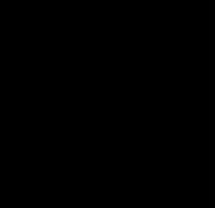
\includegraphics[scale=1.0]{./gw/greenpoles.pdf}
\end{center}
\caption{\small \label{fig:greenpoles} Pole structure 
of the Green's function. The occupied electronic states are
slightly above the real frequency axis and below the chemical 
potential $\mu$, the unoccupied states are located above the Fermi
level and slightly below the real axis. The poles of the Green's 
function correspond to the addition/removal energies 
in the system. This example is for a system with a discrete series of 
excitations and an energy gap between occupied and unoccupied states
of $E_{g}$.}
\end{figure}
%
To demonstrate this it is necessary to Fourier transform the Green's function
from the time domain to the frequency domain. This can be accomplished by 
rewriting the field operators in the Heisenberg representation:
%
\begin{equation}
\label{eq:heisenop}
\cfield(\r,t) = e^{i\hat{H}t}\cfield(\r) e^{-i\hat{H}t}.
\end{equation}
%
We then introduce a complete set of states which describe all the possible 
intermediate excitations of the system to $N'$ particles 
and their $s$ excited states,~$|N',s\ket$:
%
\begin{equation}
\label{eq:compstates}
\sum_{s}|N', s\ket \bra N',s| = \I,
\end{equation}
%
where $\I$ is the identity matrix.
We also note that:
%
\begin{equation}
H|N,s\ket = E^{s}_{N}|N,s\ket.
\end{equation}
%
%
If one inserts Eqs. \ref{eq:heisenop} and \ref{eq:compstates} into Eq.~\ref{eq:green} it is possible 
to write the Green's function in the time domain as:
%
\begin{align}
\label{eq:grtimedom}
G(\r,t,\rp,t') & = & \sum_{s} -i\Theta(t-t') e^{i(E^{0}_{N} - E_{N'}^{s})(t-t')}\bra N|\field(\r)|N',s\ket\bra N',s|\cfield(\r')|N\ket \nonumber \\
	  &+ & \sum_{s} i\Theta(t'-t) e^{-i(E_{N}^{0} - E^{s}_{N'})(t-t')}\bra N|\cfield(\r') |N',s\ket \bra N',s|\field(\r)| N \ket.
\end{align}
%
Now Eq.~\ref{eq:grtimedom} gives the Green's function in the time domain and the arguments depend 
only on differences in time $t-t'$. By introducing the time variable $\tau = t-t'$ it is 
straightforward to define a Fourier transform:
%
\begin{equation}
G(\r,\r';\omega) = \frac{1}{2\pi} \int_{-\infty}^{\infty} G(\r,\r,\tau) e^{i\omega\tau} d\tau,
\end{equation}
%
and represent the Green's function in the frequency domain:
%
\begin{eqnarray}
\label{eq:greenfreq}
G(\r,\rp;\omega) & = &\sum_{s} \frac{\bra N|\field(\r) |N',s\ket \bra N',s|\cfield(\r')| N \ket}{\omega - (E^{s}_{N'} - E^{0}_{N}) + i\delta} \nonumber \\
	  		     & - & \sum_{s}\frac{\bra N|\cfield(\r') |N',s\ket \bra N',s|\field(\r)| N \ket}{\omega + (E^{s}_{N'} - E^{0}_{N}) - i\delta}.
\end{eqnarray}
%
The infinitesimal factors of $i\delta$ ensure that the Fourier 
transform converges at infinite time arguments.
The presence of the field operators implies that the only 
non-zero contributions to Eq.~\ref{eq:greenfreq} are between 
the ground and excited states of the $N'=N+1$ and the $N'=N-1$ systems. 
Therefore it is convenient to make the follow substitution~\cite{inkson86}:
%
\begin{equation}
(E^{s}_{N+1} - E^{0}_{N}) = \epsilon^{s}_{N+1},
\end{equation}
%
with a similar expression for the $N-1$ system. The variable $\epsilon^{s}_{N\pm1}$ 
is the energy difference of an excited state in the $N\pm1$ many body system and 
the ground state of the $N\pm1$ system. 
This leads us to:
%
\begin{eqnarray}
\label{eq:greenpoles}
G(\r,\rp;\omega) = \sum_{s} \frac{\bra N|\field(\r) |N+1,s\ket \bra N+1,s|\cfield(\r')| N \ket}{\omega - \epsilon^{s}_{N+1} + i\delta} \nonumber \\
			 		-\sum_{s} \frac{\bra N|\cfield(\r')|N-1,s\ket \bra N-1,s|\field(\r)| N \ket}{\omega + \epsilon^{s}_{N-1} - i\delta}.
\end{eqnarray}
%
The poles of Eq.~\ref{eq:greenpoles} are represented schematically in Fig.~\ref{fig:greenpoles} 
and correspond to the energies of the excitations from $N$ to $N\pm1$ electrons 
in an interacting many body system. Having discussed the pole structure of 
the Green's function we now proceed to define the equation of motion.

\section{Green's function methods}
\noindent
Lars Hedin first developed the $GW$ approximation with
his publication ``New Method for Calculating the One-Particle Green's Function
with Application to the Electron-Gas Problem.''~\cite{hedin65}. In this work Hedin developed a
self-consistent system of equations for including all the interaction effects
in a many electron system. Hedin describes the
connection between his work and the development of Green's
functions methods by Schwinger in Ref.~\cite{schwinger51} 
working in the field of quantum electrodynamics.
An early review of the applications of Green's function methods and
Feynman diagrams to the many electron problem was given in Ref.~\cite{pratt63}. The procedure
has been extensively studied in the 
intervening thirty years and Refs.~\cite{aulbur00, aryasetgunnarsson98, onida02}
provide a review of the contemporary state of the field.
%
\subsection{Equation of motion}
\noindent
To derive the equation of motion for the Green's 
function we need the time derivative of Eq.~\ref{eq:green}. 
This derivative in turn requires working out the time 
dependence of the field operators appearing in Eq.~\ref{eq:green}:
%
\begin{equation}
\frac{\partial \field(\r,t)}{\partial t} = i[\hat{H},\field(\r,t)].
\end{equation}
%
The time dependence of the field operator is determined by the 
commutator between the Hamiltonian and the field operator.
%
The general Hamiltonian we will consider can be separated into two parts:
%
\begin{equation}
\H =  \H_{0} + v(\r,\r')\delta(t-t'),
\end{equation}
%
where the $\H_{0}$ term describes the kinetic energy of the electron and the interaction of the 
electron with an ionic lattice. 
The $v(\r,\r')\delta(t-t')$ term represents the inter-electron Coulomb repulsion.
We differentiate Eq.~\ref{eq:green} with respect to time to arrive at the following result:
%
\begin{align}
\label{eq:greqmotn}
\left[i\frac{\partial}{\partial t} - \H_{0}\right]G(\r,\r',t,t') +  & &  \nonumber \\
i\int v(\r,\r'')\bra N| T[\cfield(\r'',t)\field(\r'',t)\field(\r,t)\cfield(\rp,t')] |N \ket d\r'' & = & \delta(\r-\rp)\delta(t-t').
\end{align}
%
The right hand side of Eq.~\ref{eq:greqmotn} comes immediately from 
the fact that $\frac{\partial}{\partial t}\Theta(t-t') =\delta(t-t')$, 
and the anti-commutator identity for fermionic field operators. 
%
The commutator for the single particle operator, $\H_{0}$, and the 
field operator can be separated directly. 
The final term under the integral sign results from the commutator
involving the field operators and the Coulomb interaction.

The number of indices that we require to keep track of everything when 
describing multi-particle propagators, and, in the next section, 
when taking functional derivatives, can be very large. 
Therefore, in order to proceed, we will employ the compressed notation for space, 
time, and spin: $1 = (\r,t,\sigma)$, $2=(\r',t',\sigma')$, and so on.

The quantity under the integral sign in Eq.~\ref{eq:greqmotn} is a two particle Green's function:
%
\begin{equation}
\label{eq:2pgreenfxn}
G_{2}(1,2,3,4) = \frac{1}{i^{2}} \bra N|T[\cfield(4)\cfield(3)\field(2)\field(1)]|N\ket.
\end{equation}
%
Eq.~\ref{eq:greqmotn} expresses the single particle Green's function now defined 
implicitly in terms of the two particle Green's function. The two particles Green's function is 
defined in terms of  four field operators. The equation of motion for the two particle Green's 
function would then involve terms with an increasing number of field operators due to the coupling 
via the Coulomb interaction.
This is the heart of the many body problem: an infinite expansion of interaction terms,
all of comparable magnitude, due to the strength of the Coulomb coupling.

When trying to solve equations of the form Eq.~\ref{eq:greqmotn} it is convenient to 
replace the function appearing under the integral sign with a new function,
termed a kernel, and then attempt to solve the system of equations in terms of this kernel.
In order to solve Eq.~\ref{eq:greqmotn} and derive the $GW$ approximation,
we will introduce three new quantities: $\Sigma$, $P$ and $\Gamma$.
Respectively these are named the self-energy, the polarization propagator, and the vertex function.
At this stage we introduce the self-energy $\Sigma$, by rewriting the integrand in Eq.~\ref{eq:greqmotn} as:
%
\begin{equation}
\label{eq:greqmsig}
\left[i\frac{\partial}{\partial t} - \H_{0}\right]G(\r,\r',t,t') - \int \Sigma(\r,\r'',t,t'')G(\r'',\rp,t'',t')d\r''dt'' =  \delta(\r-\rp)\delta(t-t').
\end{equation}
%
The equation now has the shape that we discussed in Sec.~\ref{sec:thelda} when discussing
the generalized Kohn-Sham exchange correlation potential. The Green's 
function evolves under the single particle
interactions included in $\H_{0}$ and according to some non-local, energy dependent potential, $\Sigma$.
What remains to be done is to show how we can calculate $\Sigma$ efficiently, and remove the 
implicit definition of the Green's function in terms of multi-particle propagators.

\subsection{Functional derivative of the Green's function}
\noindent
Eq.~\ref{eq:greqmotn} defines the equation of motion for the one particle Green's
function by making reference to the two particle Green's function.
In the following we will rewrite the equation of motion so that it is entirely defined in
terms of the single particle Green's function. This can be
accomplished by relating the single particle Green's function to the two particle Green's
function via a functional derivative.

To derive Hedin's equation we make some formal modifications. The following derivation follows closely
that presented in Appendix A of Ref.~\cite{hedin65}, the review article of \cite{strinati88} 
and the textbook of Inkson \cite{inkson86}. A few important functional identities 
are reproduced in Appendix~\ref{app:funcdiv}. These are required to manipulate the equations 
and obtain their final closed form.

First Eq.~\ref{eq:greqmotn} is rewritten to include a perturbing potential $\phi(1)$:\footnote{For our
purposes a local scalar potential $\phi(1)$ is sufficient to derive the $GW$ approximation. More general 
perturbations, e.g. coupling to non-local vector potentials, are developed in Ref.~\cite{strinati88}.}
%
\begin{align}
\label{eq:greqmotn2}
\left[i\frac{\partial}{\partial t} - \H_{0} - \phi(1)\right]G(1,2) +& \nonumber \\
i\int v(1,3)\delta(t_{3}-t_{1})\bra N| T[\cfield(3)\field(3)\field(1)\cfield(2)] |N \ket d3 &= \delta(1,2).
\end{align}
%
The perturbing potential will be set to zero at the end of the derivation.

Eq.~\ref{eq:greqmotn2} allows us to separate motion generated by the original Hamiltonian, 
which is composed of the single electron and electron-electron
interaction terms, from the time development due to the perturbation $\phi(1)$. The perturbing potential 
allows us to define the functional derivative of the system's Green's
function, and hence relate the propagation of a single particle to the propagation of multiple particles. 
The introduction of $\phi(1)$ allows us to generate an infinite series of terms 
describing the electron-electron interactions in terms of functional derivatives.

Eq.~\ref{eq:greqmotn2} is rewritten so that the field operators refer to the ground-state field
operators, denoted $\field_{0}$, and their time development due to $\phi(1)$ is made explicit:
%
\begin{equation}
\label{eq:intergr}
G(1,2) =  \frac{\bra N|\hat{T}[\hat{S}\field_{0}(1)\cfield_{0}(2)]|N\ket}{\bra N| \hat{S} |N\ket}.
\end{equation}
%
The $\hat{S}$ operator propagates the ground-state field operators according to:
%
\begin{equation}
\hat{S} = T\rm{exp}\left[-i\int_{t_{1}}^{t_{2}} \phi(2)\field_{0}(2)\cfield_{0}(2)d{2}\right].
\end{equation}
%
This separation ensures the time development of the field operators due to $\phi$ is made explicit
and the field operators have no implicit dependence on the perturbation. In this way the field 
operators reflect only the dynamics of the underlying electron system interacting via the Coulomb interaction.

By functional differentiation of Eq.~\ref{eq:intergr} with respect to the perturbing potential $\phi$ 
the two particle Green's function can be written:
%
\begin{equation}
\label{eq:funcdifgr}
G(1,3,2,3^{+}) = G(1,2)G(3,3^{+}) - \frac{\delta G(1,2)}{\delta \phi(3)}.
\end{equation}
%
To arrive at Eq.~\ref{eq:funcdifgr} we used the quotient rule as it applies to functional derivatives, 
and that the variation in $S$ is:   
%
\begin{equation}
\frac{\delta \hat{S}}{\delta\phi(3)} = i \hat{S} \field(3)\cfield(3).
\end{equation}
%
We can now use Eq.~\ref{eq:funcdifgr} to replace the two particle propagator in Eq.~\ref{eq:greqmotn}:
%
\begin{align}
\label{eq:greqmwfd}
\left[i\frac{\partial}{\partial t}-\H_{0}(1)-V(1)\right]G(1,2) &
	-i\int v(1,3)\frac{\delta G(1,2)}{\phi(3)}d3 &=\delta(1,2),
\end{align}
%
where: 
%
\begin{equation}
V(1) = \phi(1) - i\int v(1,3) G(3,3^{+})d3.
\end{equation}
%
Eq.~\ref{eq:greqmwfd} has now separated into two terms. The first term
contains the single electron components
of the Hamiltonian, the perturbing potential, and what can now be
identified as the Hartree potential, i.e. the mean field
felt by an electron due to the classical potential generated from the electron cloud 
discussed in Section~\ref{sec:hohnkohn}. The connection can be seen directly 
by noting that the quantity $G(3,3^{+})$ is just the electronic density. 
\footnote{It is important to see this connection: the diagonal elements 
of the Green's function are just the electron density. 
The superscript $+$ is added to avoid problems
with the definition of the step function in the time 
domain when $(t-t')=0$.}

The second term contains the \emph{bare} Coulomb interaction 
multiplied by the functional derivative of the 
one particle Green's function. Upon comparison of 
Eq.~\ref{eq:greqmwfd} with Eq.~\ref{eq:greqmsig} we can 
rearrange terms by observing:
%
\begin{equation}
\int \Sigma(1,3)G(3,2)d3 = -i\int v(1,3) \frac{\delta G(1,2)}{\delta \phi(3)}d3,
\end{equation}
%
or by isolating the self-energy $\Sigma$ as: %(where we have used app. 1 Eq.~\ref{eq:expansionrule}):
%
\begin{equation}
\label{eq:sigma}
\Sigma(1,2) = i \int v(1,4) G(1,3) \frac{\delta G^{-1}(4,2)}{\delta\phi(4)}d3d4.
\end{equation}
%
We now retrieve the equation of motion for the Green's function 
as it appeared in Eq.~\ref{eq:greqmsig} as:
%
\begin{equation}
\label{eq:greqmsig2}
\left[i\frac{\partial}{\partial t} - \H_{0}(1) - V(1)\right]G(1,2) - i\int \Sigma(1,3)G(3,2)d3 = \delta(1,2).
\end{equation}
%
One could formally solve this equation as it stands using an iterative method, 
however it is worth noting that the resulting expansion of the self-energy $\Sigma$ 
would contain increasing powers of the bare Coulomb interaction $v$. 
It is unlikely that the resulting series will converge particularly 
quickly, if it converges at all. 
%
Therefore it is necessary to expand $\Sigma$ in a closed form without making 
reference to the perturbing potential $\phi$. In doing so the equations are rearranged so that
the bare Coulomb interaction is modified and the electrons experience 
an effective screened Coulomb interaction. In a classical picture the electrons will interact
via a Coulomb interaction screened by the system's dielectric function. 
This will be done in the next two sections.
%
\section{Hedin's equations}
\subsection{Dielectric function}
\label{sec:dielecfun}
\noindent
At this point it is useful to introduce the following functional relationships 
which define the dielectric function in a many-body system.
We will switch back to labeling time and space coordinates as $\r,t$ 
here for ease of reference with a later section (Section~\ref{sec:genfunctionals}). 

The effective potential acting on the electrons is:
%
\begin{equation}
\label{eq:internalpot}
V(\r,t) = \phi(\r,t) - i\int v(\r,\r') G(\r',\r',t,t^{+}) d\r',
\end{equation}
%
where $iG(\r',\r',t,t^{+})$ is the single particle density $n(\r')$.
%
We now define the inverse dielectric function to be the self-consistent variation 
of this effective potential with respect to the external perturbing potential:
%
\begin{equation}
\label{eq:invepsvphi}
\inveps(\r,t,\r',t') = \frac{\delta V(\r,t)}{\delta\phi(\r',t')}.
\end{equation}
%
Upon inserting Eq.~\ref{eq:internalpot} into Eq.~\ref{eq:invepsvphi} we arrive at:
%
\begin{equation}
\label{eq:simpphys}
\inveps(\r,t,\r',t') = \delta(\r-\r')\delta(t-t') + \int v(\r,\r'') \frac{\delta n(\r'',t)}{\delta\phi(\rp,t')}d\r''.
\end{equation}
%
Eq.~\ref{eq:simpphys} has a simple physical interpretation. The inverse dielectric function 
encodes the self-consistent variation in the charge density 
with respect to a variation in the potential $\phi$.
This rearrangement of charge means that the bare Coulomb interaction
 between two points is altered by the induced screening in
the interacting medium. This altered Coulomb interaction is the 
screened Coulomb interaction, and can be defined 
in terms of the inverse dielectric function as:
%
\begin{equation}
\label{eq:scrncoul}
W(\r,t,\r',t') = \int v(\r,\r'')\delta(t-t'') \frac{\delta V(\r',t')}{\delta \phi(\r'',t'')} dr''dt''.
\end{equation}
%
The screened Coulomb interaction can also be written as an integral equation: 
%
\begin{equation}
\label{eq:dysw}
W(\r,t,\r',t') =  v(\r,\r') + \int d\r''' v(\r,\r''')\int P(\r''',t,\r'',t'') W(\r'',t'',\r',t')dt''d\r''.
\end{equation}
%
where the polarizability, $P$, has been introduced:
%
\begin{equation}
P(\r,\r',t,t') = \frac{\delta n(\r',t')}{\delta V(\r,t)}.
\end{equation}
%
Alternatively we can introduce the dielectric function in its non-inverted form as:
%
\begin{equation}
\label{eq:epschap2}
\epsilon(\r,t,\rp,t') = \delta(\r-\r')\delta(t-t') - \int v(\r,\r'') P(\r'',t'',\r',t') \delta(t-t'') d\r''dt''.
\end{equation}

\subsection{Hedin's equations}
\noindent
\label{sec:hedineqs}
While the Coulomb repulsion between electrons remains the bare Coulomb interaction, 
the dielectric function provides a route to interpreting 
an auxiliary system of electrons interacting via a \emph{screened} Coulomb interaction.

In order to include this screening implicitly in the definition of the self-energy, we 
go back to the definition of $\Sigma$ in Eq.~\ref{eq:sigma}. We now use the chain 
rule to take the functional derivative of $G$ with 
respect to the total potential $V$ rather than the perturbing potential $\phi$:
%
\begin{equation}
\label{eq:funcdifsig}
\Sigma(1,2) =  i\int v(1,4) G(1,3)\frac{\delta G^{-1}(3,2)}{\delta V(5)}\frac{\delta V(5)}{\delta\phi(4)}d3d4d5.
\end{equation}
%
By comparison of Eqs. \ref{eq:invepsvphi}, \ref{eq:scrncoul}, and \ref{eq:funcdifsig} we can combine
the inverse dielectric function and the bare Coulomb interaction into the screened Coulomb interaction $W$:
%
\begin{equation}
\Sigma(1,2) =  i\int W(1,4)G(1,3)\frac{\delta G^{-1}(3,2)}{\delta V(4)}d3d4.
\end{equation}
%
The final piece of notation to be introduced is the vertex function. This is defined as the variation 
of the inverse Green's function with respect to the potential $V$:
%
\begin{equation}
\label{eq:vertex}
\Gamma(1,2;3) = \frac{\delta G^{-1}(1,2)}{\delta V(3)}.
\end{equation}
%
Having obtained the expression for the vertex function in Eq.~\ref{eq:vertex} we
can write all of Hedin's equations in a closed form.
We summarize Hedin's equations describing the interacting Green's function,
the screened Coulomb interaction, the polarizability, and the vertex function of the system:
%
\begin{align}
\label{eq:hedinsig}
&\Sigma(1,2)   = i\int W(1^{+},4)G(1,3)\Gamma(3,2;4)d4d3 &   \\
\label{eq:hedinw}
&W(1,2)        =  \int \inveps(1,3)v(3,2) d3 &               \\
\label{eq:hedineps}
&\epsilon(1,2) =  \delta(1,2) - \int v(1,3)P(3,2)d3 &        \\
\label{eq:hedinpol}
&P(1,2)        = -i\int G(1,3)\Gamma(3,4;2) G(4,1^{+})d4d3 & \\
\label{eq:hedinvert}
&\Gamma(1,2;3) = \delta(1,2)\delta(1,3) + \int \frac{\delta\Sigma(1,2)}{\delta G(4,5)}G(4,6)G(7,5) \Gamma(6,7;3)d4d5d6d7 & 
\end{align}

In summary, we started from the equation of motion. Then a relationship between
the two particle Green's function and the one particle Green's function was found.
This relationship takes the form of a functional derivative of the one particle Green's function with
respect to a perturbing potential. When everything is written in terms 
of the one particle Green's function we obtain a set of equations 
that need to be solved self-consistently. These are known as Hedin's equations. 
When solved iteratively these equations incorporate all the many body 
effects of a many-electron system.

\section{$G_0W_0$ self-energy and corrections to LDA eigenvalues}
\noindent
In the first section of this chapter we have discussed the
procedure for constructing the $G_0W_0$ self-energy operator.
We have also discussed some of the considerations required when
performing DFT calculations within a planewaves basis set.
It remains to show how the $G_0W_0$ self-energy can be
used to connect the eigenvalues obtained from a DFT calculation.

We proceed as in Ref.~\cite{HL86} by assuming the $G_0W_0$
self-energy can be treated as a perturbation to the
DFT Kohn-Sham exchange and correlation potential.

In Chapter~\ref{chap:dftgw} we discussed the quasiparticle equation:
%
\begin{equation}
\label{eq:qpeq2}
\left[-\frac{1}{2}\nabla^{2} + \hat{V}^{\rm{ion}} + \hat{V}^{\rm{H}}\right]\phi_{n\k}(\r) + \int{d}\r' \Sigma(\r,\r';E_{n\k})\phi_{n\k}(\r')=E_{n\k}\phi_{n\k}(\r).
\end{equation}
%
By adding and subtracting $V_{xc}(\r)\psi_{n\k}(\r)$ one obtains:
%
\begin{equation}
(-\frac{1}{2}\nabla^{2} + \hat{V}^{\rm{ion}} + \hat{V}^{\rm{H}} + \hat{V}^{\rm{xc}})\phi_{n\k}(\r) + \int{d}\r' \left[\Sigma(\r,\r';E_{n\k})-\hat{V}^{\rm{xc}}(\r')\delta(\r,\r')\right]\phi_{n\k}(\r') = E_{n\k}\phi_{n\k}(\r).
\end{equation}
%
If we treat $\Sigma-V^{\rm{xc}}$ as a perturbation we can express $E_{n\k}$
in terms of the Kohn-Sham eigenvalues $\epsilon^{\rm{LDA}}_{n\k}$ using 
first order perturbation theory:
%
\begin{equation}
\label{eq:QPenergy}
E_{n\k}^{\rm{QP}} = \epsilon_{n\k}^{\rm{LDA}} + \bra n\k| \Sigma(E_{n\k}^{\rm{QP}}) - \hat{V}^{\rm{xc}}|n\k\ket.
\end{equation}
%
Following Ref.~\cite{HL86} we expand the self-energy operator to first order around the LDA eigenvalue:
%
\begin{equation}
\label{eq:sigmafirst}
\Sigma( E_{nk}^{\rm{QP}} ) = \Sigma(\epsilon_{nk}^{\rm{LDA}}) + \frac{\partial\Sigma(\omega)}{\partial \omega}\bigg|_{\omega = \epsilon_{n\k}^{\rm{LDA}}}(E_{n\k}^{\rm{QP}} - \epsilon_{n\k}^{\rm{LDA}}). 
\end{equation}
%
The quasiparticle energy can than be obtained by substituting Eq.~\ref{eq:sigmafirst} into Eq.~\ref{eq:QPenergy}:
%
\begin{equation}
\label{eq:QPfirst}
E_{n\k}^{\rm{QP}} = \epsilon_{n\k}^{\rm{LDA}} + \left(1-\frac{\partial\Sigma(\omega)}{\partial \omega}\bigg|_{\omega=\epsilon_{n\k}^{\rm{LDA}}}\right)^{-1}(E_{n\k}^{\rm{QP}} - \epsilon_{n\k}^{\rm{LDA}}). 
\end{equation}
%
The quasiparticle renormalization value $Z$ is defined by:
%
\begin{equation}
Z_{n\k} =  \left[1-\frac{\partial\Sigma(\omega)}{\partial \omega}\bigg|_{\omega = \epsilon_{n\k}^{\rm{LDA}}}\right]^{-1}.
\end{equation}
%
In summary, we find the expression for the $G_{0}W_{0}$ perturbative correction to the LDA eigenvalues is:
%
\begin{equation}
\label{eq:qpcorrpert}
E^{\rm{QP}}_{n\k} =  \epsilon^{\rm{LDA}}_{n\k} + Z_{n\k}\bra n\k|\Sigma(\epsilon^{\rm{LDA}}_{n\k})-V^{xc}_{n\k}| n\k\ket.
\end{equation}
%

\section{The Spectral function}
\subsection{The $GW$ spectral function}
\label{sec:spec}
\noindent
In this section we introduce the spectral function. For simplicity we will contract the
Bl\"och notation $n\k$ to a single index $n$, and then reintroduce the full Bl\"och notation when
we arrive at the final expression for the spectral function.

Given a set of single particle eigenvectors $\phi_{m}(\r)$ we can take matrix elements of the
single particle states with the Green's function and self-energy:
%
\begin{eqnarray}
G_{mn}(\omega)       = \int \int \phi_{m}^{\star}(\r) G(\r,\r';\omega) \phi_{n}(\r')  d\r d\r', \\
\Sigma_{mn}(\omega)  = \int \int \phi_{m}^{\star}(\r) \Sigma(\r,\r';\omega) \phi_{n}(\r') d\r d\r'.
\end{eqnarray}
%
We can employ the same notation for matrix elements with $V^{\rm{xc}}(\r)$,
and the Kohn-Sham Hamiltonian $\hat{H}^{\rm{KS}}$.
%
In matrix notation the Dyson equation \cite{inkson86} can be written:
%
\begin{equation}
\label{eq:matdys}
G^{-1} = G_{0}^{-1} - [\Sigma(\omega) - V_{\rm{xc}}].
\end{equation}
%
Eq. \ref{eq:matdys} gives the expression for interacting Green's function.
We note that the exchange and correlation potential of the ground state
calculation is subtracted from the final self-energy. If the Green's function is diagonal
in the state indices we can invert each element of the matrix and write:
%
\begin{equation}
G_{nn}(\omega) = \frac{1}{\omega -\epsilon^{\rm{KS}}_{n}+{\rm Re}\Sigma_{nn}(\omega)-V^{\rm{xc}}_{nn}+{\rm Im}\Sigma_{nn}(\omega)}.
\end{equation}
%
In the case where the non-diagonal elements cannot be ignored,
a full matrix inversion would be required to construct the Green's function:
%
\begin{equation}
G_{mn}(\omega) = [\omega \delta_{mn} - \epsilon^{\rm{KS}}_{mn}\delta_{mn} + {\rm Re}\Sigma_{mn}(\omega) - V^{\rm{xc}}_{nn} + {\rm Im}\Sigma_{mn}(\omega)]^{-1}.
\end{equation}

We can employ the same notation for matrix elements with $V^{\rm{xc}}(\r)$,
and the Kohn-Sham Hamiltonian $\hat{H}^{\rm{KS}}$.
%
In matrix notation the Dyson equation \cite{inkson86} can be written:
%
\begin{equation}
\label{eq:matdys}
G^{-1} = G_{0}^{-1} - [\Sigma(\omega) - V_{\rm{xc}}].
\end{equation}
%
Eq. \ref{eq:matdys} gives the expression for interacting Green's function.
We note that the exchange and correlation potential of the ground state
calculation is subtracted from the final self-energy. If the Green's function is diagonal
in the state indices we can invert each element of the matrix and write:
%
\begin{equation}
G_{nn}(\omega) = \frac{1}{\omega -\epsilon^{\rm{KS}}_{n}+{\rm Re}\Sigma_{nn}(\omega)-V^{\rm{xc}}_{nn}+{\rm Im}\Sigma_{nn}(\omega)}.
\end{equation}
%
In the case where the non-diagonal elements cannot be ignored,
a full matrix inversion would be required to construct the Green's function:
%
\begin{equation}
G_{mn}(\omega) = [\omega \delta_{mn} - \epsilon^{\rm{KS}}_{mn}\delta_{mn} + {\rm Re}\Sigma_{mn}(\omega) - V^{\rm{xc}}_{nn} + {\rm Im}\Sigma_{mn}(\omega)]^{-1}.
\end{equation}

At this stage we introduce the spectral function by defining it in terms of the Green's function:
%
\begin{equation}
A_{mn}(\omega) = {\rm Im} |G_{mn}(\omega)|.
\end{equation}
%
Reintroducing the Bloch notation we can write the full spectral function
for the diagonal Green's function:
%
\begin{equation}
\label{eq:aspec}
A_\k(\omega) = \frac{1}{\pi}\sum_{n} \frac{|{\rm Im}\Sigma_{n\k}(\omega)|}
{[\omega- \epsilon_{n\k}-({\rm Re}\Sigma_{n\k}(\omega) -V^{\rm{xc}}_{n\k})]^{2} + \left[{\rm Im}\Sigma_{n\k}(\omega)\right]^{2}}.
\end{equation}

The spectral function helps clarify the quasiparticle picture. Eq.~\ref{eq:aspec} is strongly
peaked when the frequency $\omega$ sweeps through the renormalized
eigenvalue $\epsilon_{n\k} + {\rm Re}(\Sigma_{n\k}(\omega) - V^{\rm{xc}}_{n\k}) $. Given
the frequency dependence of $\Sigma$ additional zeros in the real part of the
denominator of Eq. \ref{eq:aspec} are possible. These can correspond to the
appearance of new excitations which are not present in the non-interacting system. Finally
the imaginary part of the self-energy introduces a broadening of the the quasiparticle peak
and is associated with lifetime effects.

\subsection{Contact with experiment}
\noindent
Angle Resolved Photoemission Spectroscopy (ARPES) is a very useful
probe for investigating the electronic structure of materials~\cite{damascelli04}.
%Incident radiation on a sample can excite electrons via the photoelectric effect. 
%These excited electrons can then propagate to a detector where their energy and momentum 
%is measured. Given the momentum and energy of the impinging light source it is 
%possible to determine the initial electronic state the captured electron occupied 
%in the material. 
%
The intensity of the electrons captured at the experimental detector, $I_{\k}(\omega)$,
can be expressed in terms of the quasiparticle spectral function~\cite{damascelli04}:
%
\begin{equation}
\label{eq:photoemission}
I_{\k}(\omega) = I_{0}(\k,\nu)f(\omega)A_{\k}(\omega),
\end{equation}
%
Where $\nu$ is the frequency of the incident radiation and $f(\omega)$ is the Fermi-Dirac distribution.
The factor $I_{0}(\k,\nu)$ includes matrix element effects, i.e.
the strength of the coupling of the initial and final electron states via
the electromagnetic probe, the effect of surfaces, and 
inelastic scattering in the sample~\cite{damascelli04}.

\subsection{Bardyszewski-Hedin theory of photoemission}
\noindent
A comprehensive analysis of the connection between the spectral function
and photoemission data is given by Bardyszewski and Hedin in Ref.~\cite{bardy85}.
Their formulation begins by relating the photocurrent, $J$, i.e. the number
of electrons ejected from the sample, per unit solid angle and energy
to the intensity, $I$, measured at the detector:
%
\begin{equation}
\frac{\partial^{2}J}{\partial \Omega \partial \epsilon_{\k}} \sim I.
\end{equation}
%
The standard definition for the intensity is then given in Refs.~\cite{goldberger64, almbladh83}:
%
\begin{equation}
\label{eq:intens}
I = \sum_{s}|\bra \k,N-1,s|\hat{\Delta}|N\ket|^{2}\delta(\epsilon_{\k}-\epsilon_{s}-\omega).
\end{equation}
%
The $|\k,N-1,s\ket$ state is a product state of the photoelectron with wave vector
$\k$ and the $|N-1, s\ket$ many electron wavefunction described in Eq. \ref{eq:compstates}.
The frequency of the incoming radiation is $\omega$. The $\hat{\Delta}$
operator is the electric dipole operator.

Eq.~\ref{eq:intens} explicitly couples many-body states via the dipole operator.
The intrinsic contribution of a particular photoelectron $\tilde{\phi}_{\k}$, to the measured photocurrent
can now be written in terms of the one-electron spectral
function discussed in Section~\ref{sec:spec}~\cite{bardy85}:
%
\begin{equation}
\label{eq:barhed}
I(\k,\omega)=\int \tilde{\phi}^{\star}_{\k}(\r)\hat{\Delta}(\r)A(\r,\r';\epsilon_\k-\omega)\hat{\Delta}(\r')\tilde{\phi}_{\k}(\r')d\r d\r'.
\end{equation}
%
If we assume the spectral function is diagonal in $\r$, $\r'$, and exploit the matrix
notation for the spectral function from the previous section we arrive at the expression:
%
\begin{equation}
I(\k,\omega) \approx \sum_{n} |\bra\tilde{\phi}_{\k}|\hat{\Delta}|\phi_{n}\ket|^{2} A_{nn}(\epsilon_{\k}-\epsilon_{n}-\omega).
\end{equation}
%
The photoelectron will not generally travel unimpeded to the detector. 
Along the way the photoelectron can scatter off of phonons, plasmons, 
or other particle-hole excitations.
Ref. \cite{bardy85} provides a detailed derivation of the 
expressions reported here for the intrinsic intensity
of the photocurrent and the possible types of quasiparticle 
excitations in an interacting system.
These results are mentioned here because they provide a direct 
connection between experimental probes and the mathematical 
formalism of the $GW$ approximation.

\section{Total Energy Functionals}
As was discussed in the introductory chapter 
a lot of work in theoretical and computational 
materials science throughout the 1980s and the early 1990s
involved sorting out the best way of computing all the terms that arise
when we need to solve the Schr\"odinger equation for a given arrangement
of atoms. This work then proceeded according to an ad hoc division of labour, 
collaborative effort, wrong turns, inventions, compromises, and synthesis 
that seems to characterize progress (or the passage of time).

To get a feel for the scale of the enterprise it is recommended that interested 
parties consult Ref.~\ref{laasonen93} which summarizes much of the progress in the field.
The reference gives a full description of how the interaction of valence electrons 
and ions are calculated, the derivatives of the many terms with 
respect to the atomic coordinates, how each term is computed in practice, 
how forces are derived in a Lagrangian formulation or in the context 
of direct minimization schemes, and the scaling of the computation with system size.
For our purposes we need only write down the total energy as a functional of
the electronic wave functions and the atomic co-ordinates:

\begin{align}
\label{eq:funcEuspp}
E^{\rm KS}_{tot}[\{\psi_i\},\{\R_{i}\}] =  & \sum_{i}\bra -\nabla^{2} + V^{NL} \ket
                                           &+ \frac{1}{2}\int\int \frac{n(\r)n(\r')}{|\r-\r'|}
                                           &+ E_{\rm xc}[n] + \int d\r V^{ion}_{loc}(\r)n(\r) + E_{ZZ}({\R_{i}})
\end{align}

There are some additional technical details that arise at this point.
The first is that the interaction of the electrons with the nuclei are handled via a pseudopotential
in this case an ultra-soft pseudopotential\cite{vanderbilt90}. The Kohn-Sham electrons are 
seeing an ionic potential given by:
%
\begin{equation}
V^{\rm NL} =  \sum_{nm,I} |\beta_{n}^{I} \ket \bra \beta_{m}^{I}|, \qquad \beta_{n} = Y^{lm}_{n}(\theta,\psi)f(R)
\end{equation}
%
The $\beta$ functions are a spherical harmonic multiplied by a radial cutoff function.

With the exception of the terms arising in the electron-ion interaction
Eq.~\ref{eq:funcEuspp} is invariant with respect to the numerical choices researchers make. 
Eq.~\ref{eq:funcEuspp} is written for the planewave-pseudopotential community:
favoured by some because the K.E. energy operator ($\nabla^{2}$) is particularly easy to evaluate, 
as is the Hartree energy, and Fast Fourier Transforms allow us to switch back and forth into whichever
representation is most convenient for any remaining terms. One could just as easily perform the calculations
in a basis of Gaussians, Slater Type Orbitals, Hankel Functions, Wavelets, or psinc functions, the list goes on.
The merits of the various techniques can be, and often are, debated at length with
robust arguments put forward from every side and actors emerging with
cross feelings over minutiae, cross feelings that may span decades. This is not to belittle the 
passionate, nigh on deranged, attention to detail the numericist insists on. 
Indeed, if we aren't careful with our calculations why should anyone believe us?

We make a second observation regarding Eq.~\ref{eq:usppEfunc}. 
One might expect that there is some universal `conservation of human effort' 
law that governs the universe. If so, reference to Eq.~\ref{eq:usppEfunc},
may spell trouble for any fitted potentials. That is an interatomic potential that makes
no attempt to solve a wave equation, and is parameterized to reproduce the accuracy
of an {\it ab initio} calculation. 

Minimization of Eq.~\ref{eq:usppEfunc} amounts to the repeated solution of sets of non-linear differential equations.
Such equations do not often suffer from a lack of solutions but rather an
over abundance of solutions\cite{haydock97}. The delicate trade-offs between 
the electronic kinetic energy and the remaining terms in the total energy, along with
the flexibility of electron waves to take new shapes means
any fitted potential will necessarily throw away the majority 
of the solution space.

Let us restate the total energy functional splitting it in two parts:
%
\begin{equation}
\label{eq:hks}
E[n] = T_{s}[n(\r)] + F[n(\r)]
\end{equation}
%
the first term is the kinetic energy contribution of the electrons, and the second is the remaining terms: 
%
\begin{equation}
F[n(\r)] = E_{\rm H}[\rho] + E_{\rm xc}[\rho] + E_{\rm e-ion}[\rho] + E_{\rm ZZ}.
\end{equation}
%

Taking the variation of Eq.~\ref{eq:hks} with respect to the density gives:
%
\begin{equation}
\frac{\delta E[n]}{\delta n} = \frac{\delta T[\rho]}{\delta \rho} + V_{\rm H}[\r] + V_{\rm xc}[\r] + V_{\rm ext}[\r] 
\end{equation}
%

Again, in the local density approximation, the exchange-correlation energy can be written:
%
\begin{equation}
E_{\rm xc}[n(\r)] = \int\epsilon_{\rm xc}[n(\r)]n(\r)dr
\end{equation}
%
By application of the chain rule the exchange-correlation potential is given as:
%
\begin{equation}
\frac{\delta E_{\rm xc}[n(\r)]}{\delta n(\r)} = \epsilon^{xc}(\r) + \frac{d \epsilon^{xc}[n(\r)]}{dn}|_{n(\r)}n(\r)
\end{equation}
%

\subsection{Harris Fragments}
Harris's approach \cite{harris85} comes from the perspective of bringing together 
"interacting fragments". As recognized by Mattheiss the one electron potential
felt by electrons in weakly correlated systems could be well approximated
by the superposition of atomic charge densities. \cite{mattheis64, haydock79}
\footnote{Similer ideas have been treated in 
K. Nikulin, Zh. Tekhn. Fiz. XLI, 41 (1971) 
[Sov. Phys. — Techn. Phys. 16, 28 (1971)]; 
R. G. Gordon and Y. S. Kim, J. Chem. Phys. 56,3122 (1972)
as well as Wendel and Martin \cite{wendel79}.}
Two separate fragments for which we can obtain the density are brought together. 
The new effective potential is generated from the sum of the fragment's densities, 
and the single particle eigenvalues are recomputed.

The idea is quite intuitive. We take a slab of one thing $n_{1}(x)$ 
and a slab of another thing $n_{2}(x)$ and form the combined density 
$n_{f}= n_1 + n_2$. From the combined density a new effective potential
is generated:

\begin{equation}
\tilde{V}(x) = V^{\rm H}(x) + \mu^{\rm nf}_{\rm xc}(x) + V^{\rm ion}(x)
\end{equation}

The eigenvalues can then be determined for the effective single particle
potential (which contains the exact configuration of ions). 
The total energy of this combined system is then given:
%
\begin{equation}
E_{R} = \sum_{i}\tilde{\epsilon_{i}} - \int d\r n_{f}[\frac{1}{2}V_{\rm H}(n_{f})+\mu_{xc}[n_{f}]+E_{\rm xc}[n_f]+E_{\rm ion}
\end{equation}
%
What has been accomplished? Well it seems a little like the trick of adding
two densities together is too simple to be useful. The usefulness lies in the
fact that when the errors introduced by the approximation 
are proportional to $\delta n(r)^2$ and not linear in the density. 

If a good guess at the density can be found, good in the sense the combined 
density is almost equal to the true self-consistent 
density, $n_{f}(r) \approx n(r)$, we have some 
grounds to think that the computed total energies will be as well
and there is no need to solve the self-consistent problem iteratively.

We will develop these ideas in the following sections but the idea of 
interacting fragments gives a useful, physically intuitive picture of
the ideas.

\subsection{Generalization of the Harris-Foulkes Functional}
The Harris-Foulkes functional:
%
\begin{equation}
E^{(1)}_{\rm HF}[\rho] = \sum_{i} \bra i |\hat{H}^{\rm in}|i\ket + E_{\rm xc}^{\rm in} - \int \rho^{\rm in}V^{\rm in}_{\rm xc} - E^{\rm in}_{H} + E_{ZZ}
\end{equation}
%
is variationally minimal with respect to the wave functions 
and with respect to the output density at fixed $rho^{in}$. 
This immediately suggests we have two co-ordinates that we can vary to minimize it. 
The effective potential is another one that can be varied $V^{in}_{eff}$.

The generalized Harris-Foulkes functional can be viewed in these terms\cite{methfessel95,haydock97}:
%
\begin{equation}
E^{HFG}[n(\r)_{\rm out}, n(\r)_{\rm in}, V_{eff}] = \sum_{i}f_{i}\epsilon_{i}-\rho^{in}V_{eff}+\rho^{in}V_{ext}+E_{xc}^{in}+E_{H}^{in}+E_{ZZ}
\end{equation}
%
The extremal properties of the Harris-Foulkes functional are discussed 
in Refs.~\cite{finnis,farid93,methfessel95, haydock97}.

To get some idea of what wandering around in this co-ordinate space,
with respect to the input density or with respective to the effective potential,
we provide in Fig.~\ref{fig:hfg} a graphical representation of the functional space.
%
\begin{figure}
\begin{center}
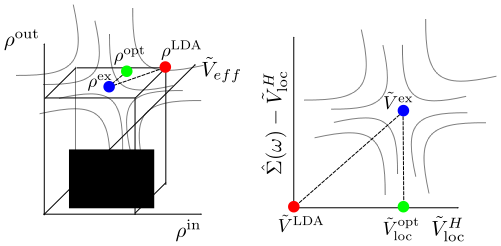
\includegraphics{./GW/HFG_space.pdf}
\caption{Schematic representation of the coordinates for the generalized
Harris-Foulkes functional. Hashed lines represent contours drawn to indicate
a saddle point. The left panel gives stationary points in the co-ordinate space
for different functionals. The blue dot indicates the stationary point for the
LDA Kohn-Sham functional with the exact density $\rho^{ex}$, 
and exact Kohn-Sham energy functional. The green dot gives a stationary point
for a hypothetical "optimal functional". The red dot is a stationary point
for the Kohn-Sham Functional using the local density approximation. 
The right panel divides the space of effective potentials into a coordinate 
composed of only local Hermitian potentials, which tend 
to be easier to work with computationally, and an orthogonal co-ordinate 
of non-Hermitian, non-local potentials, which are more problematic. 
This is in the spirit of Refs.~\cite{sohrab10, patrick12, sohrab17}. 
The figure demonstrates how one can approach an optimal
potential which minimizes the distance to the stationary point of the true interacting potential
while retaining desirable computational properties like being Hermitian and local
or allowing us to avoid multiple iterations to self-consistency.}
\end{center}
\end{figure}
%
The blue dot corresponds to $\rho^{\rm ex}$, and $V^{\rm ex}_{\rm eff}$. The red dot
represents the stationary point for the HKS functional using the LDA.

\section{Connecting Density Functional Theory and Tight Binding}
One of the reasons for the preceding discussion was to put us in
the position of being able to build our recursive tight-binding formulation
of electronic structure on the rocks of Hohenberg and Kohn's Theorem, 
variational principles, and the rock-like LDA, rather than on the 
sands of intuition, faith, interpolation, and post hoc success.

In the tight-binding formulation the total energy is decomposed into two terms:
%
\begin{equation}
\label{eq:totentb}
E_{0}^{\rm TB} = \sum_{i}\epsilon_{i} + \frac{1}{2}\sum_{\alpha} \sum_{\beta \ne \alpha}U(|R_{\alpha} -R_{\beta}|).
\end{equation}
%

We may compare this directly with the Hohenberg-Kohn-Sham expression for the total energy:
%
\begin{equation}
\label{eq:totendft}
E_{0}^{\rm DFT} = \sum_{i}\epsilon_{i} - \int \frac{\delta F}{\delta n}n(\r)d^{3}\r + F[n(\r)] 
\end{equation}
%
that is the sum over the eigenvalues of the non-interacting electron system (which gives us our kinetic
energy), minus the double counting bits, and adding the rest.

We now expand the total energy functional around a stationary density $n_0$:
%
\begin{equation}
E[n_{0} + \delta n] = E[n_{0}] + \frac{1}{2}\int\int \frac{\delta^{2} E}{\delta n(\r) \delta n(\r')} \delta n(\r)\delta n(\r')d\r d\r'
\end{equation}
%


When we begin our calculations we must choose an initial density and from this
define an initial potential, i.e. the potential the electrons see:
%
\begin{align}
V_{in}(\r)  & = \frac{\delta F} {\delta n}|_{n_in} \\
            & = V_{\rm nucl}(\r) + V_{\rm H}(n(\r)) + \mu_{xc}[n_{\rm in}(\r)]
\end{align}
%

When the auxiliary set of non-interacting electron Schr\"odinger equations are solved using this potential
a new density can be generated. We will call this $n_{\rm out}$. The total energy in terms
of $n_{\rm out}$ is written:
%
\begin{equation}
\label{eq:totennout}
E[n_{\rm out}]= \sum_{i}\epsilon_{i} - \int \frac{\delta F}{\delta n}|_n_{\rm in}n_{\rm out} d\r + F[n_{out}].
\end{equation}
%
Note well that we are accustomed to iterating the process until $n_{out}=n_{in}$, i.e.
until self consistency has been reached. The point of the present discussion is we would like
to avoid this iterative process. We would like to do less work.

%A similar potential can be obtained using an output density $n_{\rm out}$
%that is the density formed by the independent electronic wave functions
%computed from $V_{in}$.

Towards this end we now let $\Delta n = n_{out}-n_{in}$ and expand $F[n_{\rm out}]$ 
at $n_{\rm in}$ Eq.~\ref{eq:totenenout}:
%
\begin{equation}
\label{eq:toten2}
E[n_{\rm out}]= \sum_{i}\epsilon_{i} - \int \frac{\delta F}{\delta n}|_n_{\rm in}n_{\rm in} d\r + F[n_{\rm in }] 
+ \frac{1}{2}\int\int  \frac{\delta^{2} F}{\delta n^2}|_{n_{\rm in}}\Delta n \Delta n.
\end{equation}
%
A useful exercise for the reader is to start from an expansion of $E[n_{\rm in}]$
rather than $E[n_{\rm out}]$. In this case a second order expansion of the kinetic energy part of the functional. 
Grouping the first three 

Discarding the second order term gives us the Harris-Foulkes Functional: 
%
\begin{equation}
\label{eq:HF}
E^{HF}[n_{\rm in}] = \sum_{i}\epsilon_{i} - \int \frac{\delta F}{\delta n}|_n_{\rm in}n_{\rm in} d\r + F[n_{\rm in }] + O((\Delta n)^{2}), 
\end{equation}
%

The interesting feature of Eq.~\ref{eq:HF} is that by solving the non-interacting
electron equations at the input density and evaluating the total energy
at the input density we only need to expect an error that is of the 
second order in $\Delta n$.

\subsection{The Second Order Variation: Dielectric Interlude}
There is a great deal of scope for connecting the second order variation in the Kohn-Sham functional
and linear response theory. Working through the steps leads to the self-consistent tight-binding method.
For a proper development of these points the reader must consult the relevant sections of 
Finnis\cite{finnis}. 

Here we will highlight the discussion of Wendel and Martin\cite{wendel78}\footnote{It would
probably be fair to call the Harris-Foulkes functional the Wendel-Martin-Harris-Foulkes functional.} 
to make the connection between the variation of the exchange-correlation functional and 
the dielectric response of the material this is to be compared with Sec.~\ref{sec:dielfun}.

Wendel and Martin begin from the Hohenberg-Kohn scheme writing everything in terms of the total energy functional:
%
\begin{equation}
\label{eq:martin1}
E[n] =\int (v(\r)+\Delta v(\r))(n(\r)+\Delta n(\r)) + T_{s}[n(\r)+\Delta n(\r)] + F[n(\r) +\Delta n(\r)].
\end{equation}
%
and expanding this expression to second order in terms of first order variations of the external potential,
$v(\r)$, and the density, $n(\r)$. 

Expansion of Eq.~\ref{eq:martin1} leads to the following contribution to the total energy that is second order in
the small density variation.
%
\begin{equation}
\label{eq:martin2}
\frac{\delta^{2} F}{\delta n(\r) \delta n(\r')}
\Delta E^(2) = \int\int \left[\frac{1}{|\r-\r'|} + \frac{\delta^{2} T_{s}}{\delta n(\r)\delta n(\r')}+\frac{\delta^{2} E_{xc}}
{\delta n(\r)\delta n(\r')}|_{n_0}\right]{\Delta n(\r) \Delta n(\r')}
\end{equation}
%
As mentioned in Section \ref{sec:hedineqs} in the GW method we considered a system of independent electrons
interacting via a screened Coulomb interaction.

To establish the relationship between the electron-electron interactions encoded in the second order variation
of the Hartree, kinetic energy functional, and exchange-correlation functional, and the inverse dielectric constant.

Note we are now working with the static dielectric function unlike in Sec.~\ref{sec:dielecfun}
when we included the time dependence of this operator. Working with the density is a little simpler than
the Green's function.

With Harris-Foulkes we are seeking to justify the form of the tight-binding expression
for the total energy, Eq.~\ref{eq:totentb}, and ascertain the errors we expect by not iterating
our solution to self-consistency. We will complete the work of the former aim in the next section,
and we have already seen that the error will be second order in $\Delta n$. Unfortunately 
as anyone who has performed a self-consistent electronic structure calculation starting from 
atomic charge densities will know that there could be anywhere between 20 and 100 iterations 
of the whole processthe charge mixing strategies. In particular we mention the Broyden type mixing approaches 
of Vanderbilt and Louie \cite{vanderbilt84} and Johnson \cite{johnson88} which, with each
step of an iterative process, improve the approximation to the dielectric matrix.
%
\begin{equation}
\epsilon^{-1}(\r,\r') = \delta(\r-\r')  + \int d \r'' \frac{1}{|\r-\r''|}\chi(\r'',\r')
\end{equation}
%
We may view the dielectric function as the Hessian of the charge density. 
Furthermore a knowledge of the variation of Eq.~\ref{eq:dielexch} with respect 
to atomic co-ordinates encodes the harmonic vibrational and elastic properties of a system.
One suggestion would be to use the generalized HF functional to choose 
$V_{\rm in}$ to be generated from $\tilde{n}_{0}$ rather than $n_{\in}$.
%
\begin{equation}
n^{1}_{out}-n^{0}_{out} = -\chi(n_{in}^{1}-n_{in}^{0})
\end{equation}
%
We want $n^{1}_{\rm out}$
%
\begin{equation}
n^{1}_{\rm in} = n^{0}_{in} + \chi^{-1}n^{0}_{out}
\end{equation}

As a final note we point out that the Hartree Energy is quadratic in the density variation
but the exchange-correlation functional is non-linear. 
This non-linearity affects the Jacobian matrix generating new search directions.
This is important for random structure searching. If subsequent densities 
are not being modified with this non-linearity they will lead somewhere predictable. It is interesting
to contemplate whether even more general paramterizations of the exchange correlation functional
would stabilize more exotic structures. But this leads us further afield.

\subsection{Superposition of Atomic Charge Densities}
Let us now build an input density by superimposing a collection of charge densities
corresponding to a single atom: $n_{in} = \sum_{i}n_{\alpha}(R_i)$. The electrostatic
contributions to the total energy break down into a free atom Hartree term, an ionic term, 
and a valence Hartree term:
%
\begin{equation}
U_{\rm es}[n_{v}] = -E_{H}[n_{\rm atom}] + \frac{1}{2}\sum_{ij} \left[ \frac{Z_{i}Z_{j}}{|R_{i}-R_{j}|} - \int\int\frac{n_{v\alpha}(R_{i})n_{v\alpha}(R_{j})}{|\r-\r'|}d\r d\r'\right]
\end{equation}

The exchange-correlation contributions to the double-counting potential are non-linear in the charge density:
%
\begin{equation}
\label{eq:xcdc}
U_{\rm xc}[n_v] = \int[\epsilon_{xc}(n_{v})-\mu_{xc}(n_{v})]n_{v}(\r) d\r 
\end{equation}
%

To proceed Foulkes and Haydock make the assumption that if only small 
areas of the material have significant charge density contributions arising from three atom 
overlaps then Eq.\ref{eq:xcdc} can be expanded as:
%
\begin{align}
\label{eq:xcdc2}
U_{\rm xc} = \sum_{i} D_{\rm xc}[n_{v\alpha}(\R_i)] + \frac{1}{2}\sum_{ij} D_{xc}[n_{v\alpha}(\R_i) + n_{v\beta}(\R_j)] - D_{xc}[n_{v\alpha}(\R_i)]
- D_{xc}[n_{v\alpha}(\R_j)] \\ + f(\R_i,\R_j,\R_k),
\end{align}

where $f(\R_i,\R_j,\R_k)$ is a function of three atomic co-ordinates.
%Can we choose this term to cancel effectively with the neglect of three center overlap terms?

Eq. \ref{eq:esdc} and Eq.~\ref{eq:xcdc2} end the analysis.
The double counting corrections have been wrestled into a two-center 
approximation which is enough work for now. In the next chapter, Chap.~\ref{chap:wannier},
we will look at a procedure for obtaining the matrix elements of the 
Hamiltonian, $H_{i\alpha j\beta}$, required for the contribution to the total
energy arising from the electronic coordinates.

We add a brief note on what definition of the repulsive energy we are using.
As stressed by Finnis there is a crucial difference between what he terms the
repulsive {\emph band} model and the repulsive {\emph bond} model. 
In the former $U(|\R_I - \R_J|)$ is a parametric two-center 
functional fit of the double counting terms in Eq.~\ref{eq:xcdc} and Eq.~\ref{eq:xcdc2}.
He distinguishes this from the repulsive contribution that arises in the tight-binding bond model\cite{sutton88} 
favouring the latter. The distinction is made clear by noting in the {\emph bond} 
model the total energy which is described
is a cohesive energy: that is the difference between the energy of the bonded system
and the same system decomposed into individual atoms. In the band model the repulsive contribution
is parameterizing a total system energy, which is problematic in its own right and
will need to be defined by technical details of the calculation.
In the band model the charge transfer effects implicit in the use of 
the Harris-Foulkes functional at a non-selfconsistent density 
are uncompensated.  This can lead to substantial errors.
The bond model isolates energy terms that arise from the difference between a free atom and an atom
in a condensed system and imposes a local charge conservation condition on the individual atoms.
This leaves only terms that can more appropriately be handled by a pair potential to be fitted.

A further discussion of these terms had better be left until Chapter~\ref{chap:wannier}.
As will be seen we will make these on-site terms explicit in the construction 
of our local models of the electronic structure. 

\subsection{Generalized Functionals}
Haydock \cite{haydock97} has discussed a quite general functional,
$\Phi[\{\psi_{\alpha},n(\r),V_{\rm in}(\r) \}]$. The stationary points of
this functional summarize the key features for our rigorous formulation of local methods
requires and which have been discussed up to this point.

The variation of the functional with respect to the electrons 
for the auxilliary non-interacting system is zero:
%
\begin{align}
 \frac{\delta \Phi}{\psi_{\alpha}(\r)} & = \left[-\frac{1}{2}\nabla^{2} + V_{\rm in}(\r) \right]\psi_{\alpha} -\epsilon_{\alpha}\psi_{alpha}&=& 0.
\end{align}

The variation with respect to the density leads to a connection between the effective potential
the non-interacting electronic system experiences and the exchange-correlation functional.
%
\begin{align}
 \frac{\delta \Phi}{\delta n(\r)}  & =  \frac{\delta F[n(\r)]}{\delta n(\r)} - V_{\rm in}(\r) &=& 0.
\end{align}


\begin{align}
 \frac{\delta \Phi}{\delta V_{\rm in}(\r)} & = \sum_{\alpha}|\psi_{\alpha}|^{2} - n(\r) &=& 0
\end{align}

The stationary point of this function is minimal with respect to the basis set and
the density and maximal with respect to the effective potential $V_{\rm in}$ \cite{methfessel95}.
For an interesting demonstration of the variational properties with respect to the 
effective potential in the context of GW calculations see Ref.~\cite{sohrab10}.

%It is important to stress we are also free to vary the input potential:
%\begin{equation}
%E[n_{in},V_{in}] = E_{0} + \frac{1}{2} \frac{\delta^{2}}{\delta n}\delta n_{\rm out} n_{\in} 
%\frac{1}{2}\int (V[n_{\rm in}](\r) - V_{\rm in}(\r))\delta n(\r) d\r 
%\end{equation}
%The combined functional is variational and it is {\emph minimal} with respect to the density
%and {\emph maximal} with respect to the potential. See Ismail-Beigi\cite{sohrab10} and 
%Methfessel\cite{methfessel95} for some interesting numerical demonstrations of the latter property.


\subsection{Pettifor's Maps and The Structural Energy Difference Theorem}
Before concluding this chapter we will mention some of the work that has been done
to directly connect DFT, a local formulation of electronic structure and
a huge swathe of experimental data. 

We begin with David Pettifor's phenomenological structure maps \cite{pettifor84, pettifor86a},
reproduced in Fig.~\ref{fig:structuremap}. These maps represent a distinct success for 
theoretical materials science; each aspect of Ehrenreich's criteria are met.
The properties of entire homologous series can be predicted from a set of two dimensional
coordinates and the experimental comparisons are immediate.
Beyond agreement with experiment, Pettifor's structure maps take the crucial next step for 
theoretic materials science by acting as an effective guide for the creation of new materials. 

The structure maps found usage in addressing the technical challenges encountered 
when producing ductile alloys that could withstand the high temperatures in 
jet engines\cite{sutton19}. 

For a theorist each region of the structure map can be studied from first principles.  
Through the 1980s Pettifor, his co-workers, and others in the field were able to 
explain the structural trends across the range of s-p\cite{cressoni91}, p-d\cite{pettifor86b}, 
and the full range of stoichiometric AB alloys\cite{bieber81,pettifor86a}.

The alert reader will have recognized the similarity with the Lennard-Jones
potential, in some respects the first and simplest interatomic potential, 
but one that encapsulates the idea that atoms attract each other
when they are a certain distant apart and repel each 
other when they are squeezed together. Teasing out and quantifying this
atomic behaviour will be the work of the remainder of these notes. 

\section{Conclusion}
\noindent
This chapter begain by introducing the Hohenberg-Kohn theorem. This theorem,
which states the ground-state energy of an interacting electronic system 
is a functional of the charge density is the basis of density functional theory
and much of the subsequent discussion. It provides us with a theorem upon which we may
build more elaborate methods of calculation.

We have discussed various schemes for extending DFT
to describe excited state properties and give us a better treatment of
the many body problem in extended systems. We then discussed 
Along these lines we presented a detailed discussion
of the analytic properties of the Green's function and a full derivation of Hedin's
equations which defines the $GW$ approximation. Hopefully now the reason it is called
$GW$ is less mysterious \footnote{If the naming remains mysterious you 
should go back and read that section again.}.

For a given configuration of ions it is now commonplace to send a 
DFT or GW calculation off to a computing machine and within a few minutes, hours, or 
days (depending on the size of the system) come back to directories 
full of eigenvalues, charge densities, wavefunctions, forces, and total energies.
The formal transformation from these {\emph global}, total energy methods 
based on the LDA and GW to a {\emph local representation} amenable 
to being described in terms of interatomic bonds and which are 
amenable to recursion type calculations 
was begun in Sec.~\ref{sec:usefulfunctionals}. 
These ideas will be developed further throughout the rest of the book.

\chapter{Many Body Recursion}
\label{chap:manybodyrecursion}
\section{Recursive GW}
A many body Hamiltonian amenable to being written in a sparse format might look like this:
%
\begin{equation}
H = [\frac{1}{2}\nabla^{2} + \tilde{v}_{\rm loc} + \hat{\Sigma}(\r,\r';\omega)]
\end{equation}
%
	$\Sigma(\r,\r';\omega)$ is a self energy operator, it is not local and 
has an additional argument that includes the energy.
If we impose a requirement that spatial integrals over $\Sigma$ are performed in 
well defined atom centered regions of space with localized Wannier functions. 
The off diagonal elements of a tight binding Hamiltonian can be quantified as:
%
\begin{equation}
\int_{\Omega_{j}}\bra w_{i}(r-R)|\Sigma(\R,\r';\omega)|w_{j}(r-R)\ket d\r'
\end{equation}
%
	Subsequent neighbour interactions would take a similar form
with the integration region, $\Omega_{j}$ being a Wigner cell around an 
atom with its Wannier center at $\R_j$. In order for the scheme to be sensible the contributions from subsequent shells 
must be negligible. This is likely to be the case so long as either the atomic orbitals $w$ and/or $\Sigma$ 
fall off quickly enough. Which, as will become clear when we discuss
the relationship of this scheme to the GW approximation, requires 
the Green's function or the screened Coulomb interaction to be sufficiently localized.

The on-site self-interaction term can be computed as
%
\begin{equation}
\int_{\Omega_{i}}\bra w_{i}(\r-\R_{i})|\sigma(\r,\r';\omega)|w_{i}(\r-\R_{i})\ket d\r'd\r
\end{equation}
%
The self-consistency in the recursion method relies on the adjustment of the $\Sigma$ operator 
and the fewer depths of recursion required to stabilize this quantity the more efficient the
scheme can be considered.

In principle we can now compute any quantity we like that can be expressed
as a density of states, or an integral over the density of states.
The basis set may remain an issue. The localized functions will not have the 
flexibility of planes waves so if we seek the green's function in the 
region of the plasmon energies our basis set might not have the flexibility 
to describe that solution? I'll have to think about this. Ultimately the 
solution for the resolvent at those energies i.e. ${\rm Im} G_{nk}(\omega)$ should 
reproduce what I'm looking for. The test for this would be with Si, if 
I can reproduce spectral functions with TB recursion that is a legitimate 
proof of concept and would clarify the extent to which collective excitations,
plasmon, can be incorporated in TB recursion. 

Also Writing the equations in this way and the proposed method of solution
yield some post hoc justification for parameterizations of plasmon
pole models or the use of Pad\'e approximants to capture the frequency dependence
of the key operators.

Similarly the contributions of neighbours to the self-energy 
operator yields some physical insight.

\section{The Self-Energy From Multiple Greenian Elements}
  A good first order approximation to $\Sigma$ comes from the GW approximation.
We will write matrix elements of this to see the connection between the
recursion method and the calculation of $\Sigma$. It should be come apparent that computing
the self-energy requires a large table of Greenian matrix elements between states localized
on nearby atoms, far away atoms, and the entire valence and conduction band spectrums. 
This table of Greenian elements could become excessively large very quickly and requires some
rigorous procedure to map it back into a manageable scale.
%
\begin{equation}
\label{eq:sigma}
\Sigma_{ij}(\omega) = \bra\phi_{i}|\int G(\omega-\omega')W(\omega')d\omega'|\phi_{j}\ket
\end{equation}
%
We now insert the identity operator into Eq.$\sigma$ strategically and at a number of places:
%
\begin{equation}
\label{eq:sigma}
\Sigma_{ij}(\omega) = \bra\phi_{i}|\int G(\omega')\sum_{n}|\phi_{n}\ket\bra\phi_{n}|(G(\omega')|\phi_{n}\ket\bra\phi_{n}|G(-\omega')v)d\omega'|\phi_{j}\ket
\end{equation}
%
\begin{equation}
\label{eq:sigma_onsite}%need to check the frequency polarization expression
\Sigma_{ii}(\omega) = \bra\phi_{i}|\int G(\omega')\sum_{n}|\phi_{n}\ket\bra\phi_{n}|(G(\omega')|\phi_{n}\ket\bra\phi_{n}|G(-\omega')v)d\omega'|\phi_{i}\ket
\end{equation}
%
The insertion of multiple identity operators makes what we need clear. What is required 
is to tabulate the Greenian's, $G_{ij}(\omega)$, between eigenstates of the system
the non-interacting system. In {\it ab initio} calculations this requirement 
gives rise to the "sum over states" problem. Although in principle the valence
and conduction states, at every wave vector, are known their calculation and storage
is tedious, and justified truncation of the sum is problematic.

For this scheme to be workable we again stress that the system interaction
must be sufficiently local such that $Sigma_{ij}$ matrix elements can be
calculated. This corresponds to the mutual interaction of the electrons being 
short ranged. For a single particle tight binding model these off diagonal hopping
elements can be calculated and are fixed. It is this interaction we wish
to generalize slightly to allow for a component of dynamical interaction.
\section{The Project Density of Transitions}
The PDOT\cite{annett93, haydock00, haydock16} method is 
appropriate for calculating the polarizability and provides a direct physical
interpretation in a many electron system. 

Written in Hedin's scheme the polarizability 
takes the form of a term: $iGG$, in Feynman diagrams this is a bubble diagram. We need to calculate the propagator
of an electron from 1 to 2, and a hole from 2 to 1. Dimensionally, after a Fourier transform,
the polarizability has units of transition probability per unit energy. Where there are discrete
states there are discrete transitions, this would be the case for systems
that could be considered molecules, where there are continuous bands there are continuous
bands of transitions, in metallic crystals this would be the case.

Where the recursion method for the PDOS computes the final energy distribution
for a stationary state in the syste


I think Umari's operator for $|\phi\ket\bra\phi|$ would be a natural way of
approximating the necessary sums that are complimentary to the chosen
localized single particle states (both valence and low lying conduction).
We then have the continuum states as $|\phi\ket=e^{i\G\cdot\r}-<\G|w_{i}(\r-\R)>$,
with the occupied and low lying conduction manifold represented as Wannier 
functions and the $|\phi>$ states as orthogonalized plane waves.

	Although this is essentially just a rewriting of Hedin's equations
it has practical consequences. The present method eliminates
burdensome storage of what are in practice gigantic Green's function, 
screened Coulomb, and self-energy matrices. It also 
stabilizes the necessary numerical integrations and convolutions in frequency space. 
The quadrature methods used in the standard recursion theory remain applicable.

These savings are obtained at the price of a nested call stack of recursions which 
in principle must be infinite. This may seem troubling but we do intend to truncate
the level of recursion at some point and the depth of the recursive call stack should
equate to the number of terms in the self energy expansion that are required.

	Careful, justified, selection of the initial wave functions and tight binding parameters
is also required and these quantities (if they are not chosen to be analytic and approximate)
must be computed and stored. However work done on Wannier functions makes this a very
practical route. We will now embark on some numerical work in the hope that satisfactory 
results can be obtained by truncation of the recursive call stack at a manageable level. 

Finally the method requires computation of the initial stationary states of the system.

The electron addition operator:
%
\begin{equation}
[H, c^{\dagger}(t)] = -i\hbar \frac{d}{dt} c^{\dagger}(t).
\end{equation}
%
The operator will evolve into a superposition of a fraction of the 
possible transitions of the system. If a complete set of orthonormal $\{P_{\zeta}\}$ 
states is introduced the projected transitions can be written:
%
\begin{equation}
\psi_{\alpha} = \sum_{\zeta\eta} P_{\zeta}c^{\dagger}P_{\eta} \qquad \epsilon_{\alpha} = E_{\zeta} - E_{\eta}
\end{equation}
%
The PDOT is then:
%
\begin{equation}
\label{eq:ehpairs}
\mu(\epsilon) = \sum_{\alpha} \bra\psi_{\alpha}^{\dagger}|\psi_{\alpha}\ket \delta(\epsilon-\epsilon_{\alpha})
\end{equation}
%
The stationary states all have infinite lifetimes, and according to Haydock, \ref{eq:ehpairs} can
be interpreted as the probability distribution in energy for the decay of a bare electron into one dressed
with electron-hole pairs.

It is possible to formulate this in terms of discrete transitions for low energies, for high energies
the initial state is clearly going to diffuse outwards very far and result in the excitation of 
many oscillators throughout the crystal. Where the complete set of orthonormal states
hasn't been computed already (this refers to the sum over states problem) it is required to directly
calculate the PDOT. Haydock gives a prescription for this the time dependent behaviour of
an operator is given:
%
\begin{equation}
\label{eq:creationt}
c^{\dagger}(t) = e^{i\mathbf{L}t/\hbar} c^{\dagger}
\end{equation}
%

$\mathbf{L}$, the Liouvillian, is defined as a superoperator which
acts on an operator $\mathbf{x}$ as:
%
\begin{equation}
\mathbf{L} \mathbf{x} = [\mathbf{H}, \mathbf{x}]
\end{equation}
%
Eq.~\ref{eq:creationt} will only converge if the interactions are expanded in terms
of the screened interaction. The mechanics discussed in the the project density of 
transitions is equivalent to the Hedin's GW approximation, and provides a framework
for computing the renormalization in terms of local orbitals and an 
effective energy band correponding to the plasmons.

With the choices $u_{0}=c^{\dagger}/<c c^{dagger}>^{\frac{1}{2}}$, $u_{-1}=0$,
subsequent operators are:
%
\begin{equation}
\label{eq:pdotvectors}
\mathbf{u}_{n+1} = (\mathbf{L} \mathbf{u}_{n} - a_{n}-b_{n}\mathbf{u}_{n-1})/b_{n+1}
\end{equation}
%
\begin{equation}
a_{n} = \bra u^{\dagger}_{n} \mathbf{L} \mathbf{u}_{n} \ket
\end{equation}
%
\begin{equation}
b_{n+1} = \bra 
(\mathbf{L} \mathbf{u}_{n} - a_{n} \mathbf{u}_{n} - b_{n}u_{n-1})^{\dagger} 
(\mathbf{L} \mathbf{u}_{n} - a_{n} \mathbf{u}_{n} - b_{n}u_{n-1})
\ket^{\frac{1}{2}}
\end{equation}
%

This recursion rarely terminates in practice due to loss of orthogonality of
the vectors or because the subspace is too large to compute.

If the PDoT consists of a single band of transitions with a known width 
and energy,then the recurrence can be continued with constant matrix elements, $a_{n}$ and $b_{n}=b$
for $n>N$ where a and b are fit to the known band. 

For interacting bands it becomes more difficult to approximate a 
single effective energy band.

The termination of the recurrence is a very important point. 
We are interested in the excited state properties of a system (N+1, N-1) electrons
from a local perspective. In Chapter.~\ref{chap:invariance} we worked hard to collect work
justifying this perspective. A plasmon is the collective variable of the electronic system.
In a continued fraction expansion of the the PDoT more and more distance transitions are coupled
to the starting transition. In a real system the continued fraction will terminate at the surface,
however if the surface atom is changed by a small number of atomic positions it would
be very surprising if the collective plasmon modes of the cavity changed. 
Picking a value of anywhere from 30-60 moments away should help the reader to visualize this.
The contribution of successive transistion are finite, in reality there are not an infinite number
of hops, and the effect of these remote transitions can be mapped onto collective variables.

For silicon, the plasmon energy band occurs around 16 eV. This is very high compared
to the single particle excitations which occur around 1 eV. The long range $1/\r$ nature of the Coulomb
interaction means electrons are coupled over large distance.
This coupling accounts for the high excitation energy: to get the
electron cloud moving collectively requires a relatively large amount of energy.

Experience with the GW approximation indicates an effective band model works very well
for sp semiconductors \cite{godbyneeds, hybertsenlouie, bergstressen}. 
A single plasmon mode approximates the long range density of transitions, and the local
atomic environment contributions to the PDoT can then be captured directly with the standard nearest
neighbour hopping and the inclusion of the lowest energy single particle transitions.

The situation for transition metals will be more complicated but again the local approach should yield 
a tractable framework. The important low energy transitions can all be included 
as explicit single particle states in the Hamiltonian (spin resolved states). 
The remaining particle-hole renormalization would then be accounted for 
via a set of effective plasmon energy bands. It would be of interest to
see how the number and position of these effective bands can change between systems.

The projected transitions can be written:
%
\begin{equation}
\mathbf{\psi}_{\alpha} = \sum_{n} \psi_{n}(\epsilon_{\alpha})\mathbf{u}_{n}
\end{equation}
%
the sum is over the basis ${\mathbf{u}_{n}}$ generated by Eq.~\ref{eq:pdotvectors}
with coefficients generated by:

\begin{equation}
\label{eq:pdotcoeff}
\psi_{n+1}(\epsilon) = ((\epsilon-a_{n})\psi_{n}(\epsilon) - b_{n}\psi_{n-1}(\epsilon))/b_{n+1}
\end{equation}

In his paper Haydock says equation \ref{eq:pdotcoeff} has two linearly independent solutions
which can be combined to satisfy the boundary conditions on $\psi_{N+1}$ or $\psi_{-1}$ or both.
Physically I understand this as choosing where the recurrence begins and ends not completely
clear on what it implies mathematically.

The $\mathbf{u}_{0}-\mathbf{u}_{0}$ element of the resolvent is
%
\begin{eqnarray}
R(\epsilon)& = & 1/\epsilon-a_{0}-b_{1}\psi_{1}(\epsilon)/\psi_{0}(\epsilon) \\
  & = & 1/\epsilon-a_{0}-b^{2}_{1}\epsilon-a_{1}-b^{2}_{2}\epsilon ... b_{n^{2}}/epsilon-a_{n}
\end{eqnarray}
%
and finally the PDoT:
%
\begin{equation}
\mu(\epsilon) = -\bra \mathbf{c} \mathbf{c}^{\dagger}\ket {\rm Sing} \frac{R(\epsilon)}{2\pi i}
\end{equation}
%
The PDoT is the residue of the resolvent which contributes to integrals enclosing the 
real $\epsilon$-line and it is normalized to the projecting operator.

Calculating how much of the sum rule is exhausted will give a good indication
of the effectiveness of a single band approximation, or what is equivalent,
the truncation of the recursion at a suitable number of moments.

Finally a note from the perspective of plane waves and pseudopotentials. For
highly excited conduction band states. The Bloch periodic wave function is
essentially a plane wave or free electron state. This is equivalent to saying for
sufficiently high energy states the kinetic energy is the dominant term in the Hamiltonian.
For these plane wave states the Wannier transformation is a psinc function. These psincs
give a local representation of high energy plasmon modes.




\section{Appeal of A Local Formulation of Many Body Quantum Systems}
 A resonance or transition in k-space corresponds to an excitation 
of a crystalline eigenstate but the physical meaning of this is hard to access. Highly
localized states in $\k$-space correspond to relatively diffuse regions in real space. Where
transitions are formulated in terms of the local atomic environment the process becomes slightly
more intuitive. An electron creation/destruction operator $u_{0}$ places/removes an electron in the 
first available excited/occupied state with eigenvalue $a_{0}$ in a particular unit cell. 
In terms of energy the operator takes the system to the energy 
of the $E_{N\pm1}$ interacting system. 

Eq.~\ref{eq:pdotvectors} will contain the contributions of the localized
wave packets in a vector $u_{\alpha}$ that corresponds to the resonance 
$\epsilon_{\alpha}$. In an inverse photoemission experiment the $u_{\alpha}$ chain
will come from the commutator of an electron creation operator, for a photoemission
experiment the chain of vectors in the excitation will correspond to creating a hole
in the electron system. An electronic wave packet interacts with its neighbours becoming
``dressed" by the nearby excitations of electron hole pairs. 

In a photoemission experiment real electric currents will be moving through the crystal as well.
Only the $\k$-component of the localized wave packet, at a given energy, will move through the crystal as 
an approximate eigenstate and can pass through without scattering so much that it can't be detected.
When the wave packet reaches the surface it can continue propagating
or be scattered back into the crystal, if it is to continue propagating the appropriate matrix element
is between the plane wave of the appropriate wave vector and the localized wave packet along with some
surface potential.

Other processes mean the excited state can hop 
to its nearest neighbour leaving behind a hole. The recursive formula means
the coefficients of the continued fraction and the vectors are generated at
each step and the energy dependence of the interaction can be calculated 
in a closed form. The trade off is the recursion depth must be sufficient to
pick up all the relevant poles of the interaction. For collective modes
the recursion depth would have to proceed to an impracticable depth which
is why we must map these contributions onto effective energy bands, collective
variables, or plasmon modes (depending on how you prefer to call them). 
The technique demonstrates the mathematical and physical justification 
of the plasmon as a mathematical transformation or collective excitation.

The hole state and the excited state will also interact according 
to the Coulomb interaction, these are excitons, the radius of their (potentially) 
bound state being determined by the strength of the screened coulomb interaction 
and the shapes of the electron and hole wave function. 
However the PDoT we are considering at the moment is just a single electron creation operator.
To calculate the PDoT for the electron hole system would require a 
two particle Green's function operator with a new pole in the spectrum forming
at the energy of the electron hole bound state.

\section{Mori Memory Function}
\label{sec:morimemory}
  As noted in Ref.~\cite{annett94} there is a close connection between the PDOT
formalism and Mori's memory function. 

Interestingly when working on the diffusion
of hydrogen in a lattice I realised I would require a way of computing the
inverse Laplace transform of the continued fraction generated 
using Haydock's method. A quick search later and one of the first items to come up
was a paper titled "A Continued-Fraction Representation of the Time-Correlation
Functions" the first line of the abstract was, "A continued-fraction expansion of the Laplace
transform of the time-correlation functions is obtained...". It is very nice when a problem
arises where all you have to do is go to the shop and grab the solution off the shelf.

Like many store bought items some element of self-assembly is required. In this
section we wish to simplify Mori's analysis as much as possible so that we can directly 
apply the mathematical machinery of translating a continued fraction representation of
a diffusion problem into the time domain and extract measurable quantities.

The inner product, or matrix elements required to generate the coefficients 
$a_{n}$ and $b_{n}$ in Mori's approach are generalized to include a thermal averaging:
%\begin{equation}
%\label{eq:moriinner}
%(F, G^{*})= \frac{1}{\beta} \int_{0}^{\beta} \bra e^{\lambda H)Fe^{-\lambda H}G^{*}\ket d\lambda
%\end{equation}
There is a further computational advantage here. Though the inner product in Eq.\ref{eq:moriinner}
looks complicated, in fact, it only has the effect of altering the coefficients entering
the hopping matrix. This means the laplace transform computed from the continued fraction,
and the quantum mechanical hopping parameters can be computed separately.

Mori's formula allows us to interpret the spectral function in two ways. The first is as
a purely phenomenological one of an electron in a material being excited and as it passes through
a crystal on the way to a detector being scattered by the characteristic scattering modes of the
system. The electron from its initial bound state can interact with the many body system via
the plasmon modes available to it.

The second is to interpret the probe as measuring a statistical distribution of the 
renormalized many-body electron states which have spectral weight across the full
interacting energy spectrum. 

The former, via the Mori picture, is similar to the treatment of a free particle path
being modified by its interaction with atoms in what is termed Brownian motion. In the
case of a fermion in a crystal we are looking at its `brownian motion' as it interacts
with bosons on its way to a detector.


\chapter{Off Diagonal Long Range Order}
\label{chap:odlro}
\section{Application to Long Range Off Diagonal Order}
The advantage of tight binding is it allows us to think about
the electronic structure of materials in a purely coordinate space representation.
Coordinate space is familiar in the sense we can discuss an electron as being
"here or there". This contrasts with the more familiar, at least when discussing crystals,
formalism of $\k$ space where all electronic eigenstates in a crystal are indexed by
their wavenumber. In $\k$ space an electron can be found anywhere in a crystal which
is somewhat frustrating. 

To justify the local representation we appeal unto the invariance theorem discussed 
by Heine and introduced in Chapter~\ref{chap:invariance}.

Having done all this work to get a local picture of the electronic structure of materials
it should be pointed out that many of the most interesting states of matter can't 
be understood in purely local terms. Among the most interesting state is the
superconducting state.

As an example Yang for ordered materials the local diagonal order present in crystalline materials,
represented by the matrix elements of $\rho_{1}$ (the single particle density matrix),
can result in the creation of macroscopic variables like the stress and strain.
What are the macroscopic analogs for off diagonal long range order?

C. N. Yang's work provides what I consider the most accessible treatment of long range
correlations in quantum systems and some of the important results and observations about
the nature of the crystalline and superconducting states are discussed in this chapter. 

\section{Yang's Off Diagonal Long Range Order}
Progessively higher density matrices are written with index n. 

Yang's insight is condensed in the following quotation.
%
\begin{quote}
It thus seems that in a macroscopic system, ODLRO can set in 
at $\rho_{n}$. The theorems of II indicate that
the reduced density matrix, to be called $\rho_{m}$, of lowest
order which has ODLRO must operate on a basic group that consists 
of an even number of fermions and any number of bosons. For liquid He II the basic
group is the He atom; for superconductors the basic group is a set of two electrons.
For $\rho_{m}$ the largest eigenvalue is of the order of N. It has an ODLRO
in the sense that in coordinate representation, when the unprimed coordinates are
microscopically close to a point $\x$, and the primed coordinates are microscopically
close to another point $\x'$. with $\x$ and $\x'$ macroscopically apart, $rho_{m}$
remains nonvanishing. For fixed unprimed coordinates microscopically
close together, the region of the primed coordinates where
$\rho_{m}$ remains nonvanishing is thus a "tube" with one 3-space dimension 
extending macroscopically. The volume of the region is 
\end{quote}
\begin{equation}
\Omega \times ({\rm microscopic\ dimension})^{m-1}
\end{equation}
%

The analogy Yang points out between Bloch's solution for wavefunctions 
in a crystal is also worth repeating in its entirety.

\begin{quote}
  The difference in the behavior of $R$ under changes in $\Phi$ for the cases 
with and without ODLRO is quite similar to the Bloch eigenvalue problem
in a periodic potential. Bloch showed that wave functions should be sought 
that changes by a phase factor $e^{i\Phi}$ for each lattice displacement. How does the 
wave function depend on $\Phi$? If the wave function remains finite between lattice points, 
the energy value and the wave function would be dependent on $\Phi$. If, however, 
the wave function becomes very small in a region between lattice points, 
caused by, e.g., a potential barrier, then the energy and the wave function 
would not be very much dependent on $\Phi$. For an infinite potential barrier in 
between the atoms, the wave function vanishes in the barrier, and the energy 
levels would be independent of $\Phi$ while the
wave function only picks up phase factors $e^{i\Phi}$ from one atom to the next.

The physical meaning of the effect of the presence of ODLRO on the 
phase condition (36) is the, ODLRO preserves the memory of phases over 
macroscopic distances. Also in this sense, one can interpret for the 
Bloch problem, the effect of the small nonvanishing interatomic 
value of the wave function on the C dependence of the energy: 
The nonvanishing interatomic value of the wave function preserves the 
memory of phases from one atom to the next.
\end{quote}

The wave functions dependence on $\k$ will be determined by how small 
the wave function amplitude becomes between unit cells.

This paper gives the first description of Bloch's function I have really understood. 
It also provides a sound mathematical basis for the pairing mechanism in BCS
superconductivity in the proof of Theorem 6 which Yang gives in the appendix.
%The R spacing argument can be applied to the electrons. The strip equivalent
%is microscopic (around the atom) but the spacing between phase locked electrons
%is of the order of the lattice constant.

In one way, Yang's formulation implies that the superconducting state
should be no more surprising than the formation of the solid crystalline state.

\section{Phonons}
The computation of the electron-phonon interactions in transition metals
can be computed using a tight binding formalism Ref.~\cite{varma79}.
In that work it is pointed out that d electrons form sharp resonances around
atoms but decay into plane wave states outside a localized atom so there
is a very delicate interplay between the electron being localized on an atom
and itinerant in the lattice. 
The hybridization of the d electrons with s-p electrons can also become 
significant.

\section{Antiresonance and Fano effects}
For a discussion of the Anderson model, AntiResonances, and the interaction of s and p channels
with d electrons see Ref.~\cite{terakura77}. Is an antiresonance a bit like what Anderson
talks about with electrons avoiding each other in space at a site? This is the super-exchange
mechanism he discusses?

The calculation of EPME (electron phonon matrix elements) and the computation 
of dielectric responses in a Wannier Basis are studied in \cite{terakura77}
and \cite{hank76}.

An early study at low temperature on Cu$_{2}$O\cite{white78}. An interesting study would
be to look at MgB2, cuprates, and pnictides to see all the studies which missed
the emergence of superconductivity at relatively high temperatures.


%\chapter{Metallurgy}
  Cottrell noted that metallurgy would require a "theory... which explains
the properties of metallic solids and the explanation of the origin of this
structure from the structures of individual atoms." 

Similarly Heine noted "What we lack is a fundamental quantum 
theory of the cohesion and structure of a wide diversity of solids." 

One of the main thrusts of this, increasingly misnamed note, is that the route
to a comprehensive framework for a quantum theory of cohesion must come
from a mathematically rigorous description of electronic structure based
on the local atomic environment. 

\section{Single Particle Recursion: Lave Phases}

\section{Many Body Recursion: Cohesive Properties}
For a hubbard U model of cohesion energies in FCC and HCP metal using the Project density of transitions
\cite{haydock14}.

\section{Random Alloys}
Lattice periodicity allows for the use of Bloch's theorem. The Fourier transform
is well defined and the eigenstates can be grouped according the their Bloch vector.
%
\begin{equation}
H_{nm} = e_{n}\delta_{nm} + V_{nm}
\end{equation}
%
It is also possible to consider the Fourier transform from a Bayesian perspective
where we are picking out features of a distribution with varying amounts of noise.

Mookerjee and Haydock extended the recursion method to the case of random alloys.
The developement of the recursion method to handle random material systems is 
itself quite ingenious \cite{mookerjee , haydock74}. The Hamiltonian is extended
so that tight binding hops on a real lattice are made along with potential hops
on a "field" lattice. The field lattice can be cast in tridiagonal form to represent
the underlying statistical distribution of the random alloy. Different graphs are available
to represent rectangular random distributions, binary distributions, Gaussian distributions
etc. Fig.~\ref{fig:fieldsite.png} gives an example of the first few hops on a "field-site" 
lattice to obtain the averaged value of a Green's function. The hopping of the recursion method
is now coupling lattice sites and taking into account the underlying distribution of 
the underlying parameters.
%
%\begin{figure}
%\caption{Field-Site lattice to directly compute the average quantities in a tight binding formalism}
%\end{figure}
%
Despite its elegance the number of paths now emanating from an initial orbital are
considerable and simplifying approximations need to be found due to the difficulty of 
enumerating all the possible paths through the lattice and the along the field vectors.

\section{Embrittlement of Metallic Surfaces}
Haydock has also introduced a mechanism analogous to the polaron model for describing the
"covalentization" of metallic bonds that is a potential mechanism for the embrittlement
of metals \cite{haydock82}.

\section{Mechanics}
For a study of the effect of impurity concentration on the velocity of dislocations in semiconductors see \cite{frisch67}.

%\chapter{Bayesian Materials Science}
Mention GAP models, empirical pseudopotentials, the lave phase stuff as well.
Parameters of excitation and structure TB recursions can be updated as well.


\bibliographystyle{cj}
\bibliography{./bibli/biblio.bib}
\end{document}

